\documentclass[../main/main.tex]{subfiles}
\begin{document}
%\dominitoc
%\faketableofcontents
\setcounter{chapter}{7}
\chapter{Modélisation de scène et extraction de sources}\label{ch:res}
\minitoc
\vspace{2cm}
Ce chapitre est consacré à la description de la dernière étape du pipeline \hypergal, la
modélisation de scène. Les chapitres précédents ont permis dans un
premier temps la
construction du cube intrinsèque de la galaxie hôte. Puis nous avons
procédé à sa projection dans
l'espace spectral de la SEDm à partir de la réponse impulsionnelle
spectrale de l'instrument. Enfin, nous avons également construit un modèle
de PSF robuste permettant la modélisation de sources ponctuelles.

Dans ce chapite, nous allons tout d'abord détailler le processus de
modélisation de scène, puis nous présenterons les résultats d'extraction des
différentes composantes qui la composent. Après avoir montré ces
résultats pour un cas idéal, nous montrerons quelques extractions de cas
plus complexes obtenues avec \hypergal.
\newpage

\section{Modélisation de scène}
% \label{sec:xxx}

\subsection{Présentation de la méthode}
%\label{sec:xxx}

La modélisation de scène implémentée dans \hypergal\ va globalement
suivre la méthode utilisée pour l'extraction de source ponctuelle,
présentée dans le chapitre précédent. Les cubes de données (observations) utilisés sont
préalablement calibrés en flux, en utilisant la courbe de sensibilité
inverse obtenue à partir de l'étoile standard observée la plus
récente. Les rayons cosmiques sont également retirés à l'aide du module
\pkg{ByeCr} \citep{Kimcontsep}.

L'idée est de modéliser la scène pour $N$ méta-tranches couvrant un
domaine spectral pertinent de la SEDm. En effectuant un ajustement de la
scène pour chaque méta-tranche, nous obtiendrons un jeu de
$N$ paramètres. Puis, à l'instar de la méthode d'extraction de source
ponctuelle, nous procèderons à un ajustement de la chromaticité des
différentes composantes de la scène. Cela nous permettra de fixer tous
les paramètres de forme et de position. Enfin nous terminerons par un ajustement linéaire
des amplitudes pour toutes les tranches du cube de données.

Cette procédure nécessite dans un premier temps de projeter notre cube
intrinsèque dans l'espace de la SEDm. Nous rappelons qu'à l'issue de la
détermination de la réponse impulsionnelle spectrale (LSF), nous avons
déjà projeté notre cube intrinsèque dans l'espace spectral de la
SEDm. Il nous manque donc la projection dans l'espace spatiale.

\subsection{Projection du cube intrinsèque}
%\label{sec:xxx}

La projection du cube ne se fait pas en une opération, mais en projetant
successivement chaque tranche qui le compose.

Il nous faut pour cela prendre en compte la géométrie des spaxels des 2
cubes. Pour les traitements géométriques, nous utilisons le module
\pkg{shapely}\footnote{\url{https://github.com/shapely/shapely}} \citep{shapely2007}, qui
nous permet de reconstruire la grille avec les spaxels carrés du cube
intrinsèque, et celle avec les spaxels hexagonaux du cube de données
SEDm.

Avant de projeter le flux, nous adaptons l'échelle des pixels entre les
deux espaces. Nous savons que les pixels des images PS1 ont une taille
de $0\farcs25$ de côté. Afin de connaître précisément le facteur
d'échelle à appliquer, nous avons effectué une analyse spatiale sur des
observations de la SEDm avec un grand nombre ($>3$) de sources dans le
champ de vue. Par comparaison géométrique avec les images PS1 de la même
zone du ciel, analogue à une triangulation, nous avons déterminé un
rapport d'échelle de $2.230\pm0.003$ entre la taille des pixels de la
SEDm et des images PS1. Nous en avons déduit une taille effective des
spaxels hexagonaux de $0\farcs558$/spaxel. Il est important de
comprendre que cette adaptation d'échelle est purement numérique et ne correspond pas à
un ré-échantillonnage. La Figure~\ref{fig:scaleadapted} illustre
l'importance de prendre en compte cette différence de taille entre les spaxels.

\begin{figure}[ht]
  \centering
  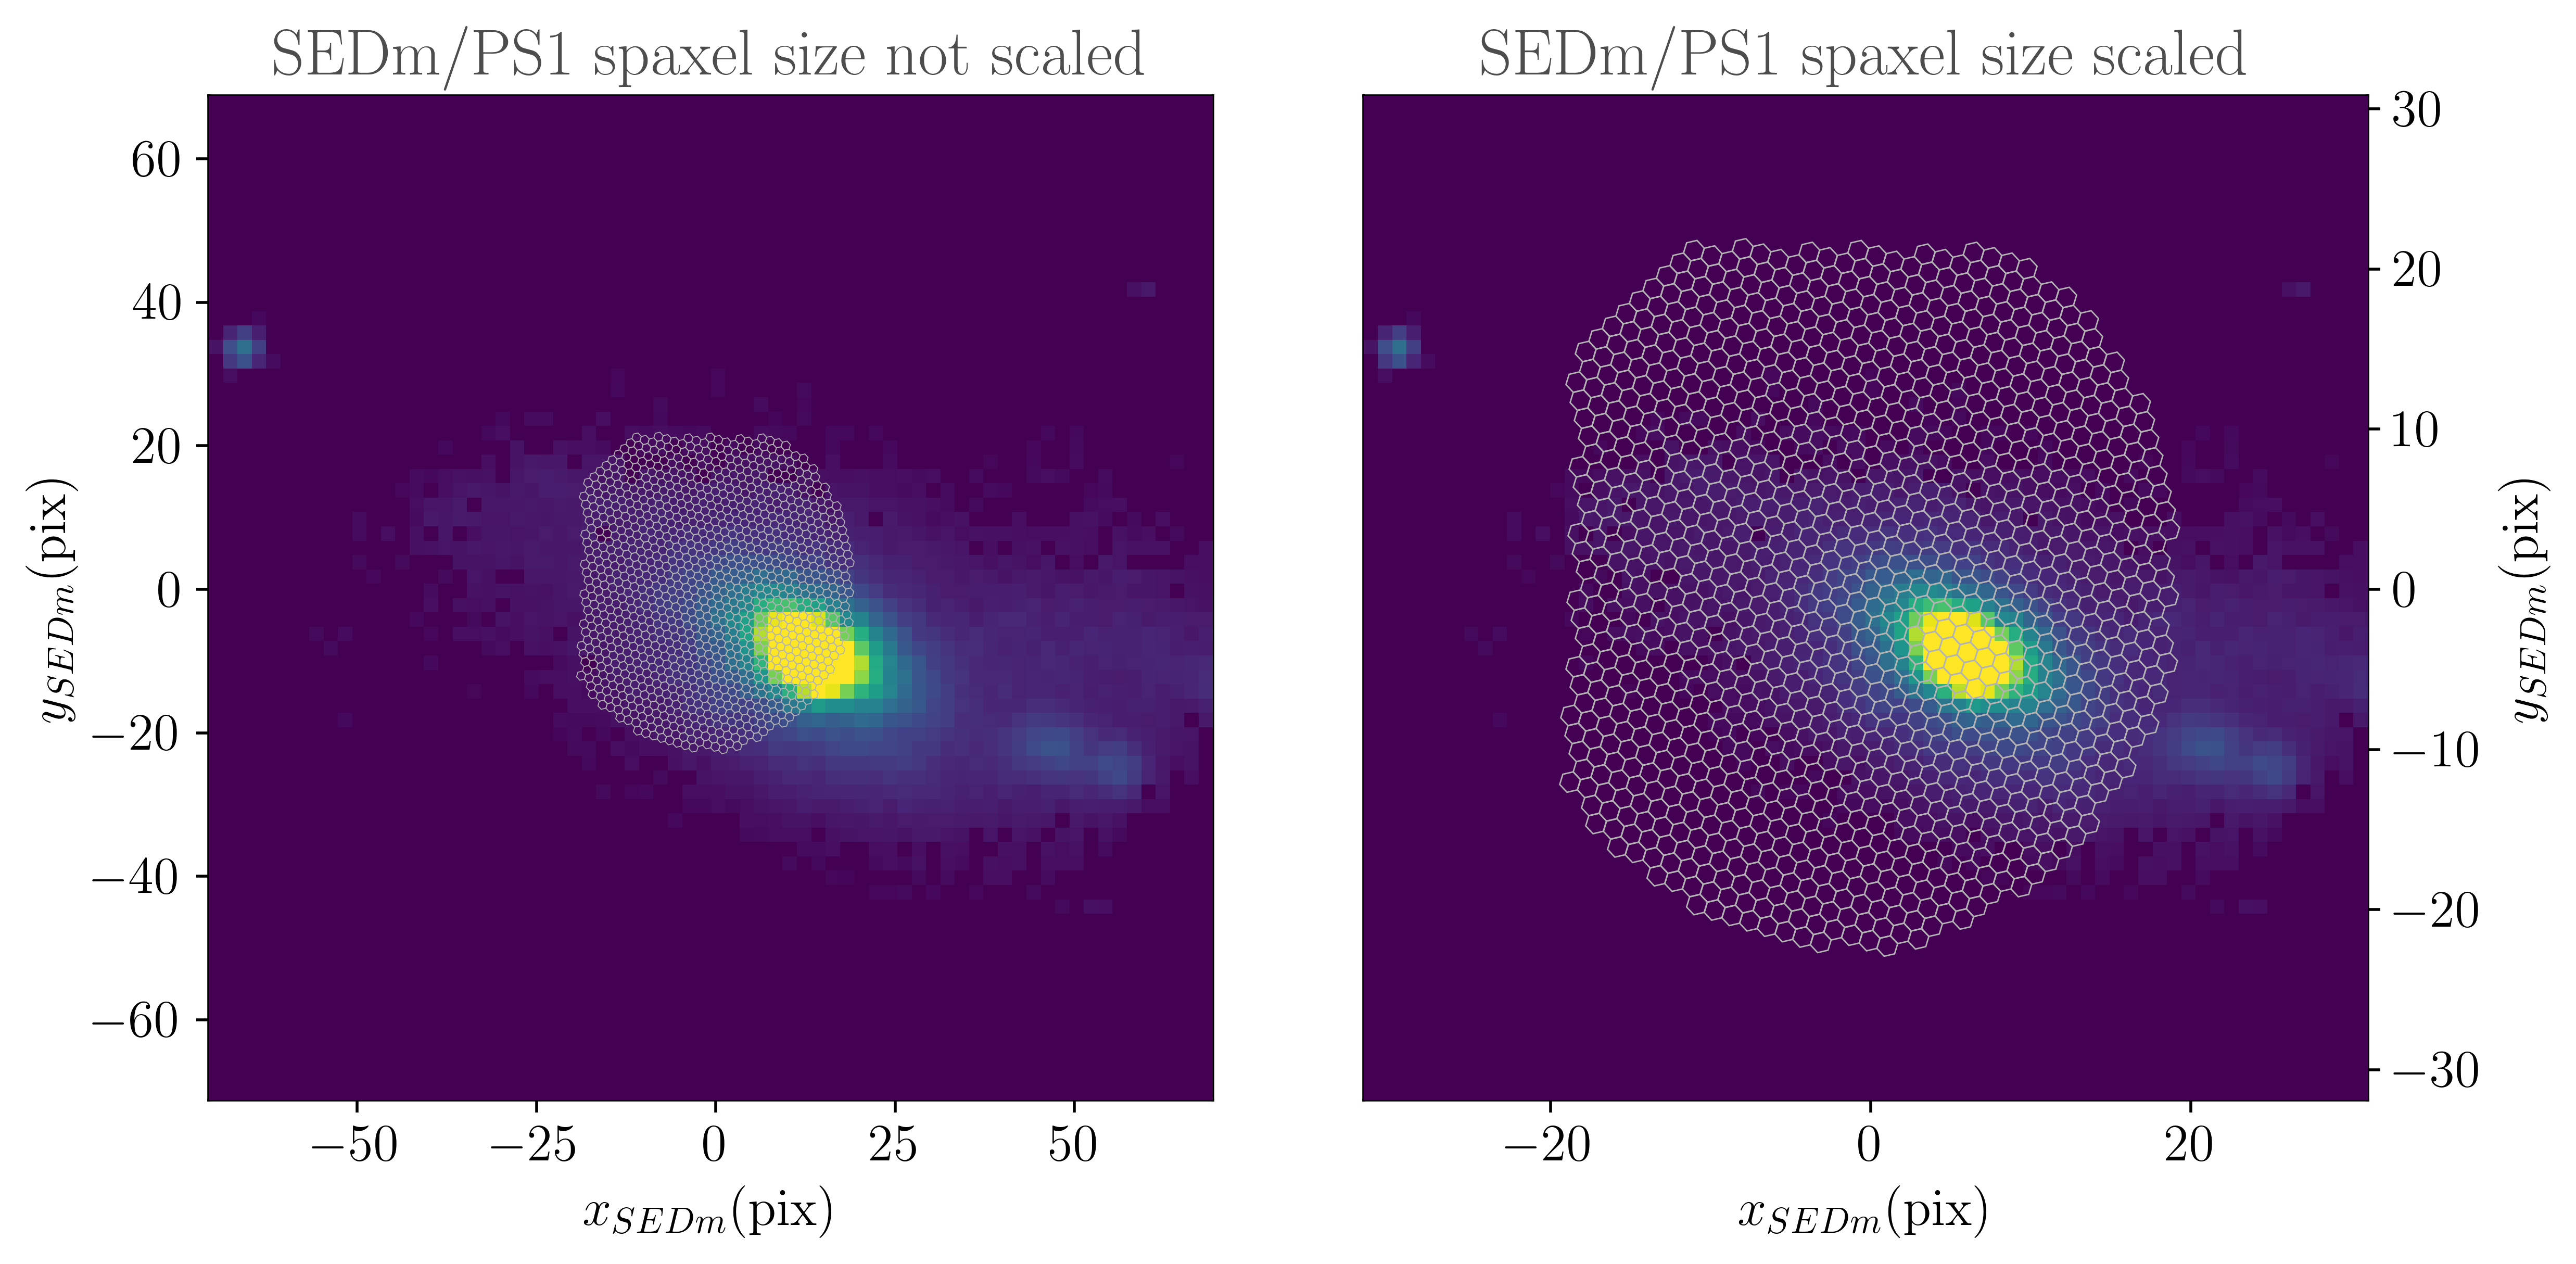
\includegraphics[width=0.9\textwidth]{../figures/07_scene/scaleadapted.png}
  \caption[Concordance des champs de vue PS1 et SEDm.]{Concordance des
    champs de vue PS1 et SEDm sur la supernova ZTF18accrorf en appliquant le rapport d'échelle entre
    la taille des pixels de chaque instrument. La grille hexagonale
    correspond au MLA de la SEDm, superposé sur une méta-tranche du cube
    intrinsèque empilé. La superposition illustrée ici aligne le centre
    du MLA et celui du cube.}
  \label{fig:scaleadapted}
\end{figure}

Avant de projeter le flux du cube intrinsèque, nous incluons un modèle de
correction du seeing. En effet, les images PS1 ayant un seeing plus
petit ($\sim1\farcs2$) que celui de la SEDm ($\sim2\arcsec$), nous
devons prendre en compte cette différence avant le ré-échantillonnage
spatial.

En toute rigueur, il faudrait entraîner un modèle de PSF relatif entre
PS1 et la SEDm. Dans ce travail, nous avons supposé que la correction du
seeing relatif pouvait être modélisée par une gaussienne 2D asymétrique
(présentant une potentielle ellipticité). Le seeing des images PS1 et
de la SEDm n'étant pas fixes, les paramètres de ce modèle seront libres
dans notre modélisation de scène.

Après la convolution de la tranche considérée du cube intrinsèque par ce
kernel gaussien, nous devons déterminer une position d'ancrage entre la
grille hexagonale et la tranche du cube à projeter.

Cette ancre de projection doit être une position du ciel dont nous
connaissons la localisation à la fois dans les images PS1, et dans le
MLA de la SEDm. Par défaut dans \hypergal, nous utilisons la position
de l'évènement transitoire détectée par la caméra ZTF, à partir de
laquelle nous avons récupéré les images PS1. La caméra de guidage de la
SEDm (la \textit{Rainbow Camera}) nous fournit également une position
approximative de l'objet détecté dans le MLA.

Nous alignons ainsi cette position du MLA avec le centre de la tranche
du cube considérée avant d'effectuer la projection du flux.

Pour procéder à la projection du flux dans l'espace spatial de la SEDm,
nous utilisons le module
\pkg{geopandas}\footnote{\url{https://geopandas.org/}}
\citep{kelsey_jordahl_2020_3946761}.
Cet outil nous permet de superposer les deux grilles de polygones
décrivant les géométries du cube intrinsèque et du MLA, puis de
déterminer les aires de chevauchement entre tous les pixels. 

Nous récupérons ainsi pour chaque pixel du MLA l'intégrale des flux
du cube qui le chevauchent, en pondérant
par l'aire de superposition. Cette aire de superposition est égale à $1$
lorsque qu'un pixel carré du cube est entièrement contenu dans un pixel
hexagonal du MLA.

Nous présentons dans la Figure~\ref{fig:projecthost} la projection d'une
méta-tranche du cube intrinsèque dans l'espace de la SEDm, convoluée par
une gaussienne 2D sans ellipticité d'écart type 1 pixel ($=0\farcs5$). L'ancrage est effectué à
partir de la position de la supernova ZTF18accrorf dans le MLA estimée
par la caméra de guidage. 

\begin{figure}[ht]
  \centering
  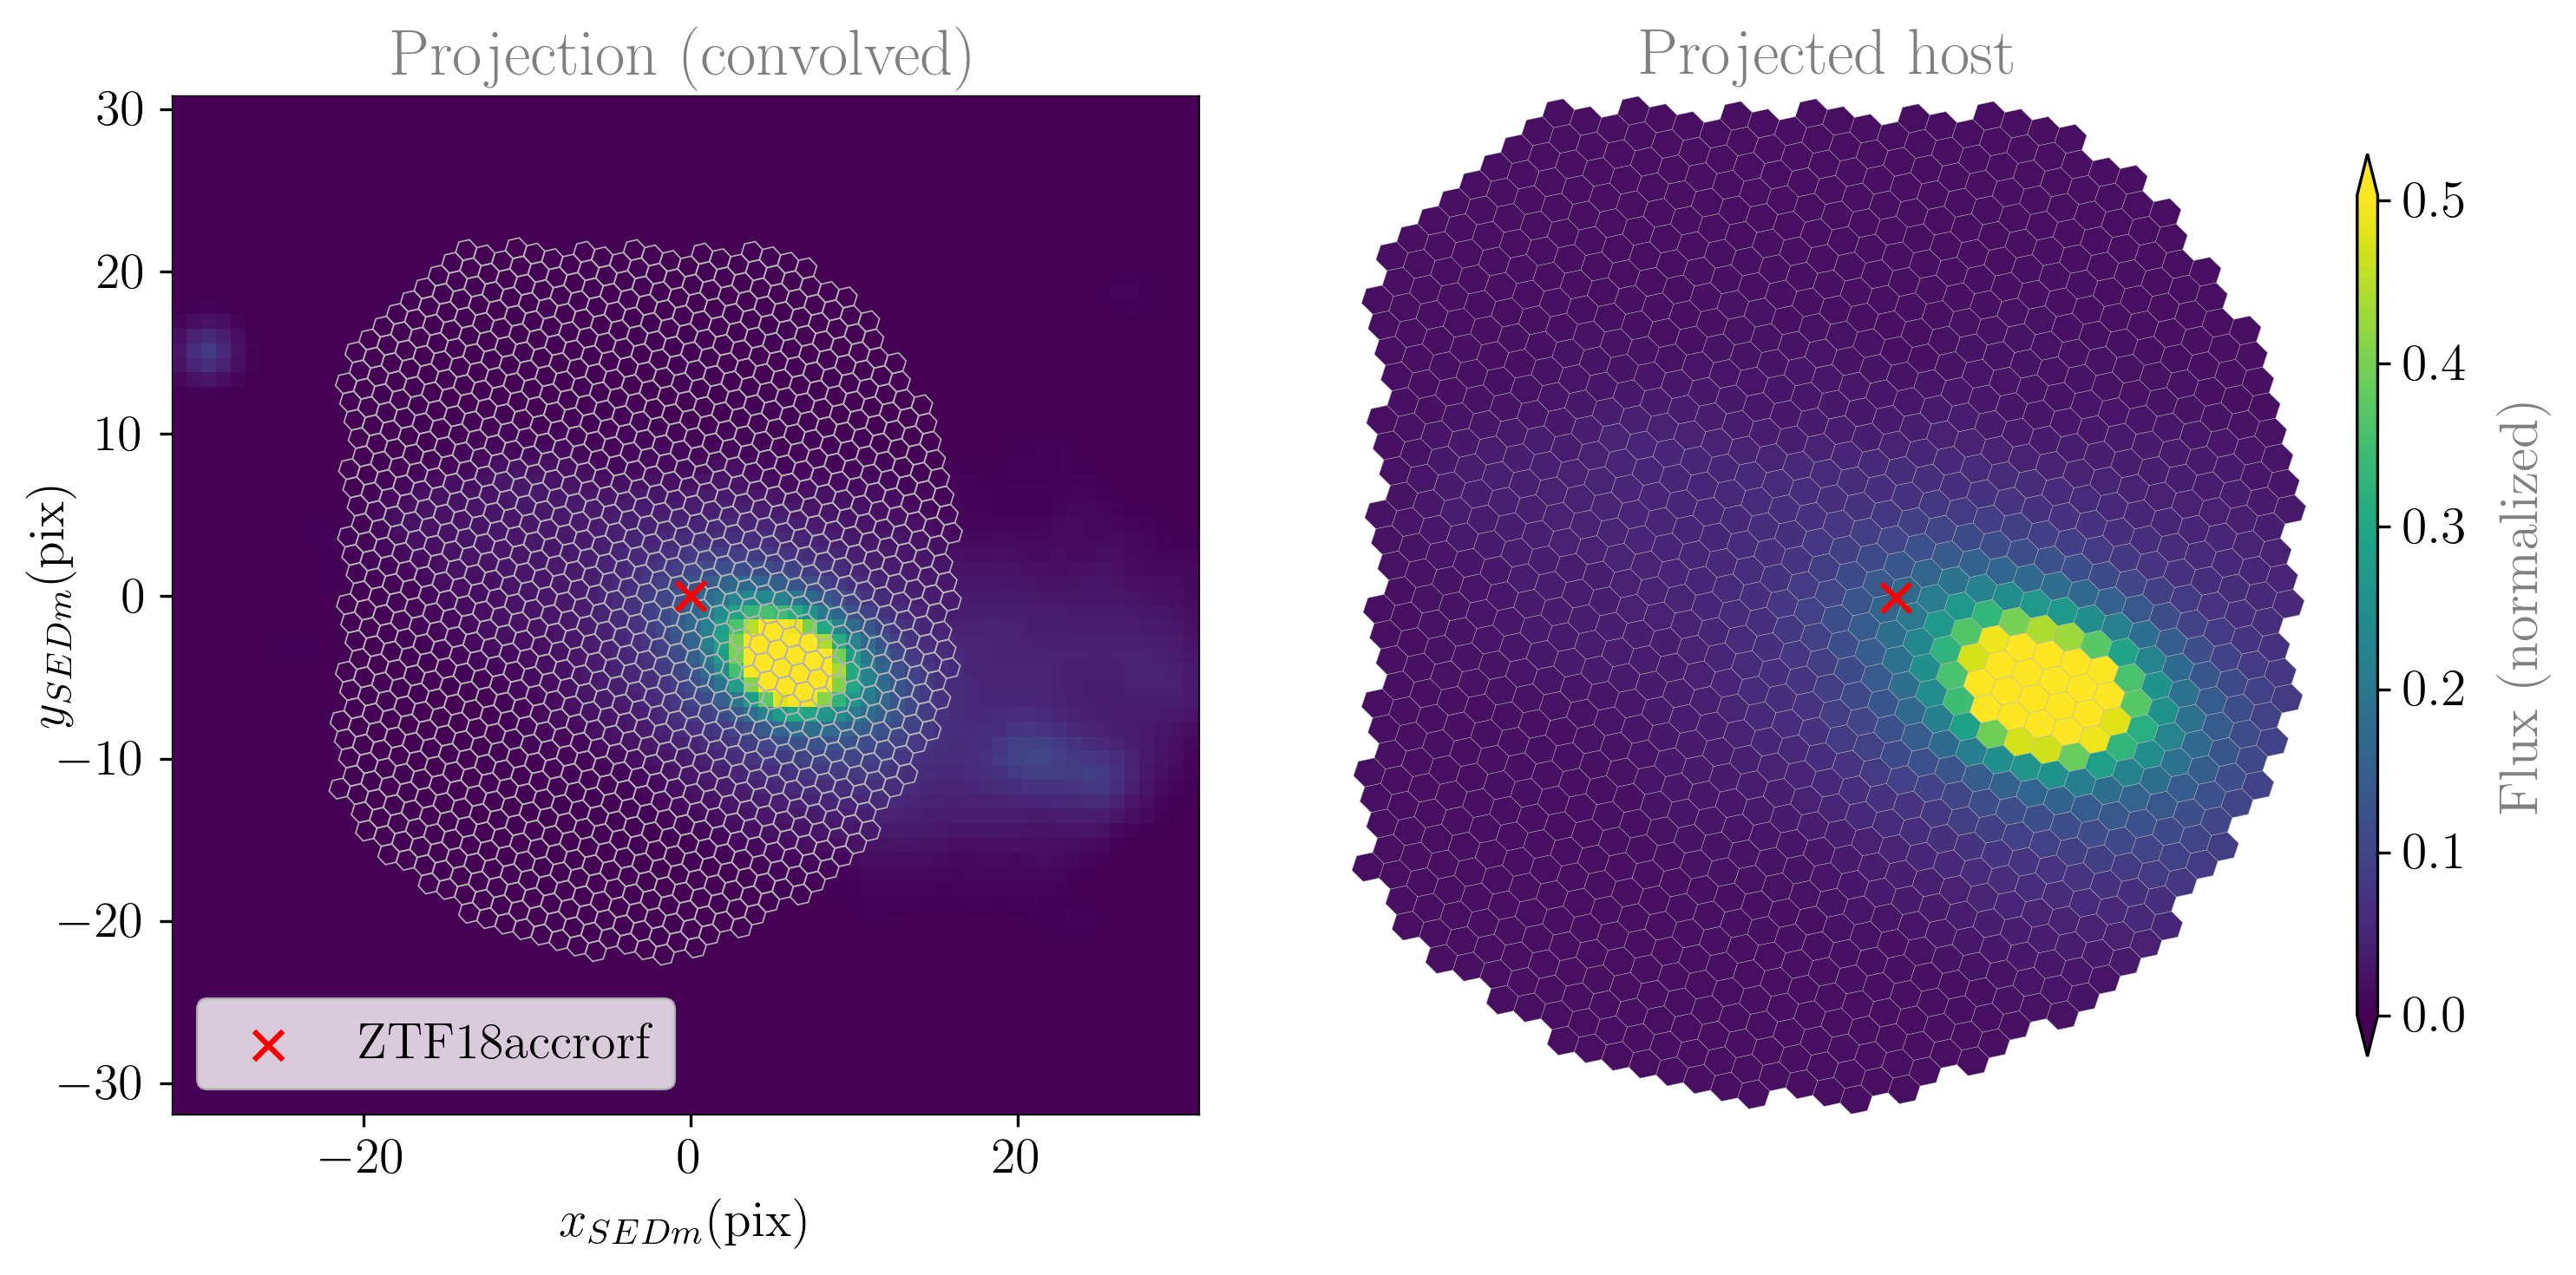
\includegraphics[width=0.9\textwidth]{../figures/07_scene/projecthost.png}
  \caption[Projection de la galaxie hôte dans le MLA.]{Projection de la
    galaxie hôte dans le MLA pour une méta-tranche du cube
    intrinsèque. Pour l'illustration de cet example, nous avons convolué la tranche par une
    gaussienne 2D sans ellipticité d'écart type 1 pixel. La croix rouge indique la position de la supernova
    ZTF18accrorf estimée par la \textit{Rainbow Camera} dans le MLA, qui
    sert d'ancrage à la projection d'un espace spatial à l'autre.}
  \label{fig:projecthost}
\end{figure}

Nous procédons ainsi à cette projection pour chaque méta-tranche du cube
spectral. Tout comme avec les étoiles standards, les 
cubes de données SEDm sont affectés par les effets d'ADR, et ainsi la position d'ancrage varie en fonction de la
longueur d'onde.

Ces paramètres ($x_{0}$, $y_{0}$) sont donc également des paramètres
libres de notre modélisation de scène, et la position renseignée par la
\textit{Rainbow Camera} fait office de condition initiale.

À ce stade de la modélisation, toutes les contributions relatives entre
PS1 et la SEDm ont été prises en compte.
Nous pouvons à présent compléter la scène avec les composantes de fond
et de source ponctuelle.

\subsection{Composantes de la scène}

\subsubsection{Composante du fond: ciel et artefacts}
% \label{ssec:xxx}

Le fond du ciel ayant été retiré dans les images PS1 \citep{Waters2020},
il nous faut modéliser cette composante. Pour les mêmes raisons évoquées
dans le chapitre~\ref{ch:irf} avec l'extraction des étoiles standards,
nous choisissons de modéliser le fond par un polynome de second degrée
tel que:

\begin{equation}
  \label{eq:backgroundcurved2}
  \text{Bkgd}(x,y) =
  \begin{pmatrix}
    b_{xx} &  &  &  &  & \\ 
     & b_{yy} &  &  &  \makebox(0,0){\text{\huge0}} & \\ 
     &  & b_{xy} &  & & \\
     &  &  & b_{x} &  & \\ 
     & \makebox(0,0){\text{\huge0}}  &  &  & b_{y} & \\ 
     &  &  &  &  & b_{0}\\
  \end{pmatrix}
  % 
  \begin{pmatrix}
    x^{2}\\
    y^{2}\\
    xy \\
    x \\
    y \\
    1 \\
  \end{pmatrix}
\end{equation}
avec $x$ et $y$ les coordonnées dans le MLA. La constante $b_{0}$ est
donc utilisée pour modéliser l'uniformité du ciel, tandis que les autres
paramètres sont là pour corriger les artefacts présents dans le cube de données.

\subsubsection{Composante de la supernova}
% \label{ssec:xxx}

L'autre composante de la scène n'est autre que la supernova, une source
ponctuelle entièrement caractérisée par la PSF de la SEDm. Nous
utilisons donc bien évidemment le profil radial contraint établit au
chapitre~\ref{ch:irf}:
\begin{equation}
  \label{eq:psfmodelconstraint}
  PSF(r; \alpha, \eta) = N\left[\eta\times\exp\left(- \frac{r}{2(\sigma_{0}+\sigma_{1}\times\alpha)^{2}}\right) +
    \left( 1+\left( \frac{r}{\alpha}\right)^{2}\right)^{-(\beta_{0}+\beta_{1}\times\alpha)} \right]
\end{equation}
avec $r$ le rayon elliptique du profil radial, et les $\sigma_{i}$ et
$\beta_{i}$ fixés par l'entraînement du modèle.

La position de la
supernova à modéliser dans le MLA est supposée confondu avec la position
d'ancrage utilisée lors de la projection du cube intrinsèque. Cette
approximation signifie que nous considérons la position de détection
dans le ciel par la caméra ZTF suffisament précise et ne nécessitant pas de
donner de liberté à la position relative entre la galaxie et l'objet
détecté.

\subsection{Ajustement de la scene 2D}
% \label{ssec:xxx}

Toutes les composantes de la scène ayant été décrites, nous pouvons
passer à l'ajustement de la scène 2D, en considérant les méta-tranches
indépendamment les unes des autres.

Nous avons choisi par défaut dans \hypergal\ de considérer 6
méta-tranches dans l'intervalle
spectral $\lambda\in$[$5000$,$8500$]\AA. Ce choix est motivé par la
précision spectrale de la calibration en flux de la
Figure~\ref{fig:allratio_std} du chapitre précédent. Bien que notre
modèle de fond ait été conçu pour prévenir de potentiels artefacts
strucutrés, ceux-ci deviennent parfois trop intenses au delà de ce domaine
spectral. En se restreignant à cet intervalle, nous réduisons le risque
de valeurs d'ajustements aberrantes pouvant compliquer par la suite l'ajustement
chromatique. De plus, la majorité des supernovae observées par la
SEDm sont des SNIea ($\sim75\%$), dont leur magnitude diminue fortement
vers le rouge, notamment au delà
de $8000$-$8500$\AA. Le contraste entre une SNIa et sa galaxie hôte dans une
méta-tranche au delà de ces valeurs est donc fortement réduit, ce qui
permet difficilement la contrainte sur les paramètres de forme de la
PSF. La Figure~\ref{fig:artefactssedmcube} illustre bien le type
d'artefacts auxquels nous faisons référence, notamment sur les bords des
cubes dans le bleu, et des franges d'interférences intenses dans le rouge.

\begin{figure}[ht]
  \centering
  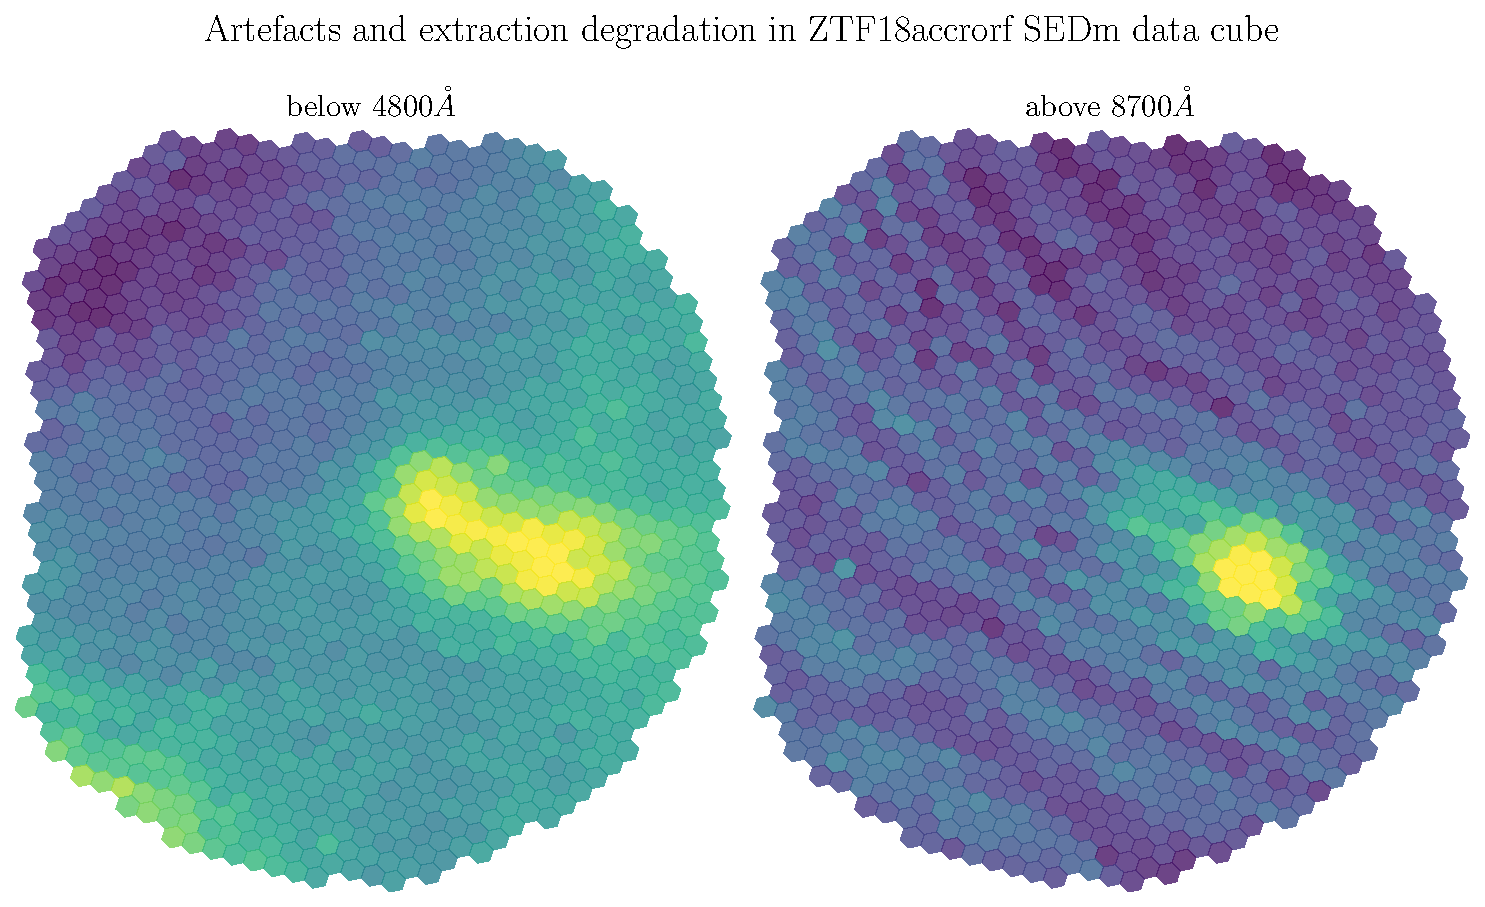
\includegraphics[width=0.6\textwidth]{../figures/07_scene/artefactssedmcube.pdf}
  \caption[Exemple d'artefacts dans les cubes de données SEDm.]{Exemple
    d'artefacts dans les cubes de données SEDm pour
    ZTF18accrorf. Nous montrons \emph{à gauche} toutes les tranches en dessous de
    $4800$\AA\ du cube de données empilées, et \emph{à droite}, toutes celles au dessus de
    $8700$\AA. Nous pouvons clairement voir dans le bleu la dégradation
    importante du signal, distordant complètement les objets dans le
    champ de vue, et également la présence d'artefacts de fond sur les
    bords du cube. Dans le rouge la forme des sources est également
    altérée, mais nous voyons surtout des franges d'interférences dans
    les données.}
  \label{fig:artefactssedmcube}
\end{figure}

Nous présentons dans la Table~\ref{tab:paramshypergal} la liste des
paramètres libres de la modélisation de scène pour une méta-tranche.
\begin{table}
  \scriptsize
  \centerfloat
  \setlength\tabcolsep{14pt}
  \renewcommand{\arraystretch}{1.5}
  \begin{threeparttable}
    \caption[Paramètres de modélisation de scène 2D avec \hypergal.]{Paramètres de modélisation de scène incluant toutes les
      composantes pour une méta-tranche dans \hypergal.}
    \label{tab:paramshypergal}
    \begin{tabular}{ccc}
      \toprule                               
      \textbf{Paramètre} &  & \textbf{Symbole} \\            
      \midrule
                         &\textbf{Géométrie}& \\
      \hline 
      Position d'ancrage  & & $x_{0}$, $y_{0}$\\
      
      \hline
      
                         &\textbf{Galaxie hôte}& \\
      
      \hline
      PSF relative SEDm/PS1 &  & $\sigma$ \\
      Ellipticité (PSF relative) &  & $\mathcal{A}_{G}$, $\mathcal{B}_{G}$\\
      Amplitude & & $G$\\
      
      \hline                               

                         &\textbf{Fond}& \\
      \hline
      
      Artefacts& & $b_{xx}$, $b_{yy}$, $b_{xy}$, $b_{x}$, $b_{y}$\\
      Ciel & & $b_{0}$\\
      
      \hline
                         &\textbf{Source ponctuelle (SN)}&\\
      
      \hline
      PSF SEDm  & & $\alpha$, $\eta$\\
      
      Ellipticité (PSF) &  & $\mathcal{A}$, $\mathcal{B}$\\
      Amplitude & & $I$ \\
      
      \bottomrule
    \end{tabular}
    \begin{tablenotes}[flushleft]
    \item \textbf{Note.} Les paramètres d'amplitudes et de fond sont
      des paramètres de nuisance dans la modélisation des méta-tranches. 
    \end{tablenotes}
  \end{threeparttable}
\end{table}

L'ajustement se fait par minimisation de $\chi^{2}$, défini comme:

\begin{equation}
  \label{eq:chi2hypergal}
  \chi^{2}=\sum\limits_{pixel}\left(\frac{(y_{p} - \widetilde{y}_{p})^{2}}{\sigma_{p}^{2}}\right)
\end{equation}
où $y_{p}$ et $\sigma_{p}$ sont respectivement le flux et la racine de
la variance dans un pixel $p$ de la méta-tranche du cube SEDm, et
$\widetilde{y}_{p}$ le flux modélisé dans ce même pixel.
Nous effectuons la minimisation avec le module
\pkg{iminuit}\footnote{\url{https://iminuit.readthedocs.io/en/stable/}} \citep{James:1975dr,iminuit}.

La procédure de construction de la scène pour une méta-tranche et pour
chaque pas de minimisation du $\chi^{2}$ se fait de la façon
suivante:

\begin{minipage}{\textwidth}%
  \begin{enumerate}[(a)]
    \itemsep=0em
  \item Convolution de la méta-tranche du cube intrinsèque par un kernel
    gaussien 2D asymétrique avec un paramètre d'amplitude;
  \item Projection dans l'espace spatiale de la SEDm suivant à partir de
    la position d'ancrage;
  \item Ajout du fond structuré (ciel + artefacts);
  \item Ajout de la source ponctuelle (PSF + amplitude);
  \item Détermination du $\chi^{2}$, puis réitération des étapes précédentes;
  \end{enumerate}
\end{minipage}\\

Nous présentons dans la Figure~\ref{fig:metaslicescene} l'ajustement des
$6$ méta-tranches par \hypergal\ pour ZTF18accrorf. Pour chaque longueur
d'onde, nous montrons la scène ajustée, la scène observée, et le résidu
avec le RMS spatial associé. Dans le cas de cette observation, notre RMS
spatial varie de $1.8\%$ à $3.9\%$. Nous pouvons également remarquer
l'augmentation de RMS pour la méta-tranche la plus \textit{bleue}
centrée sur $5285$\AA, probablement à cause d'un fond de plus en plus
structuré comme illustré dans la Figure~\ref{fig:artefactssedmcube}. La
méta-tranche la plus \textit{rouge} à $8200$\AA\ commence également à
présenter des artefacts structurés, vraisemblablement des franges de
Moiré (phénomène d'interférences).

\begin{figure}
  \centering
  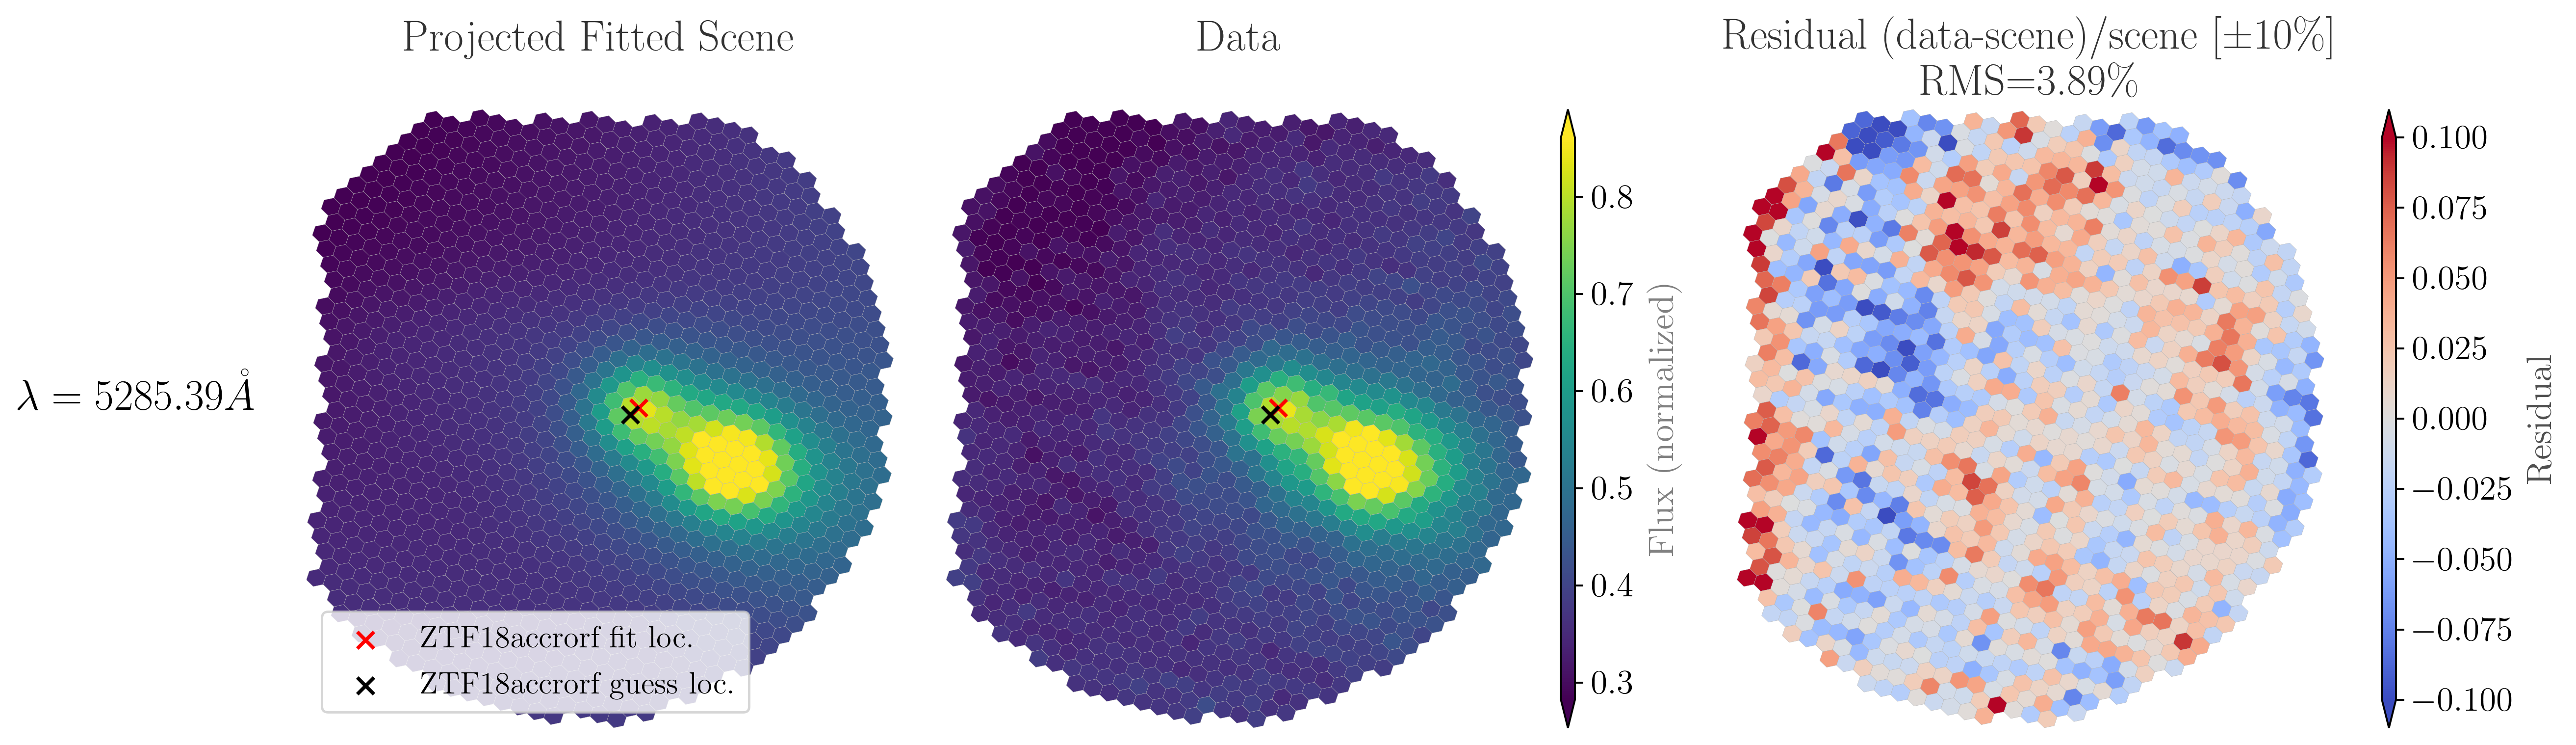
\includegraphics[width=0.8\textwidth]{../figures/07_scene/fitted_metasliceZTF18accrorf_0.png}
  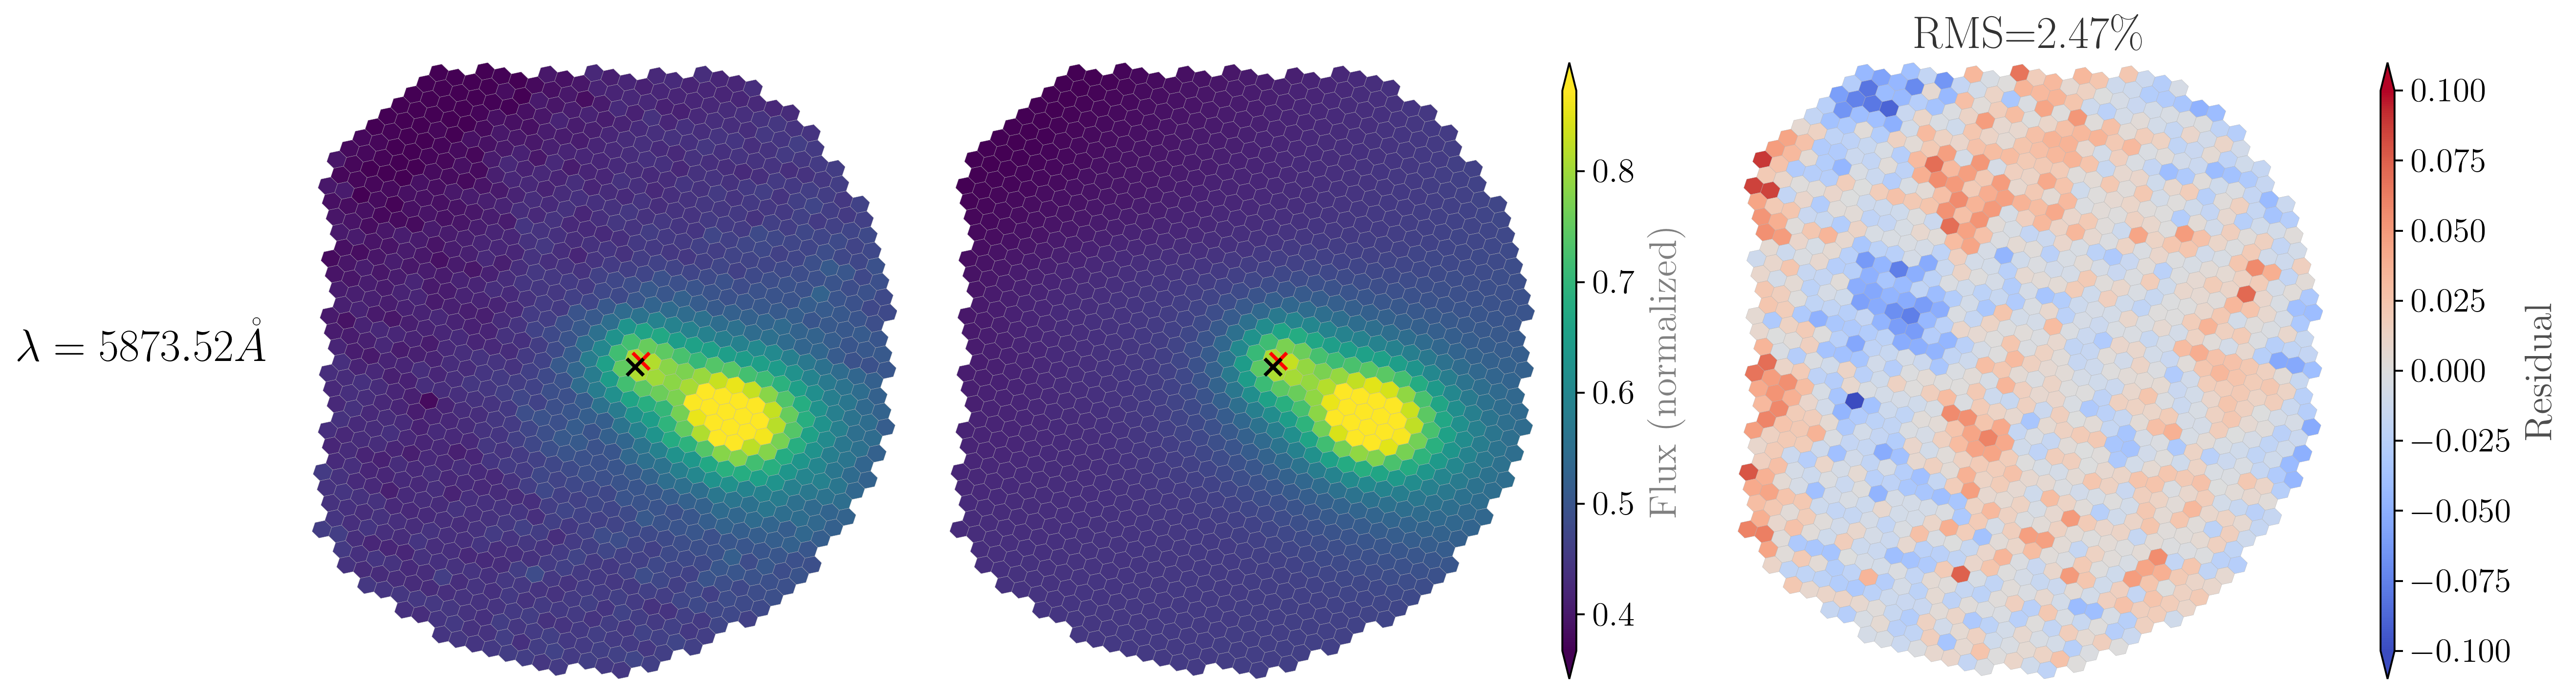
\includegraphics[width=0.8\textwidth]{../figures/07_scene/fitted_metasliceZTF18accrorf_1.png}
  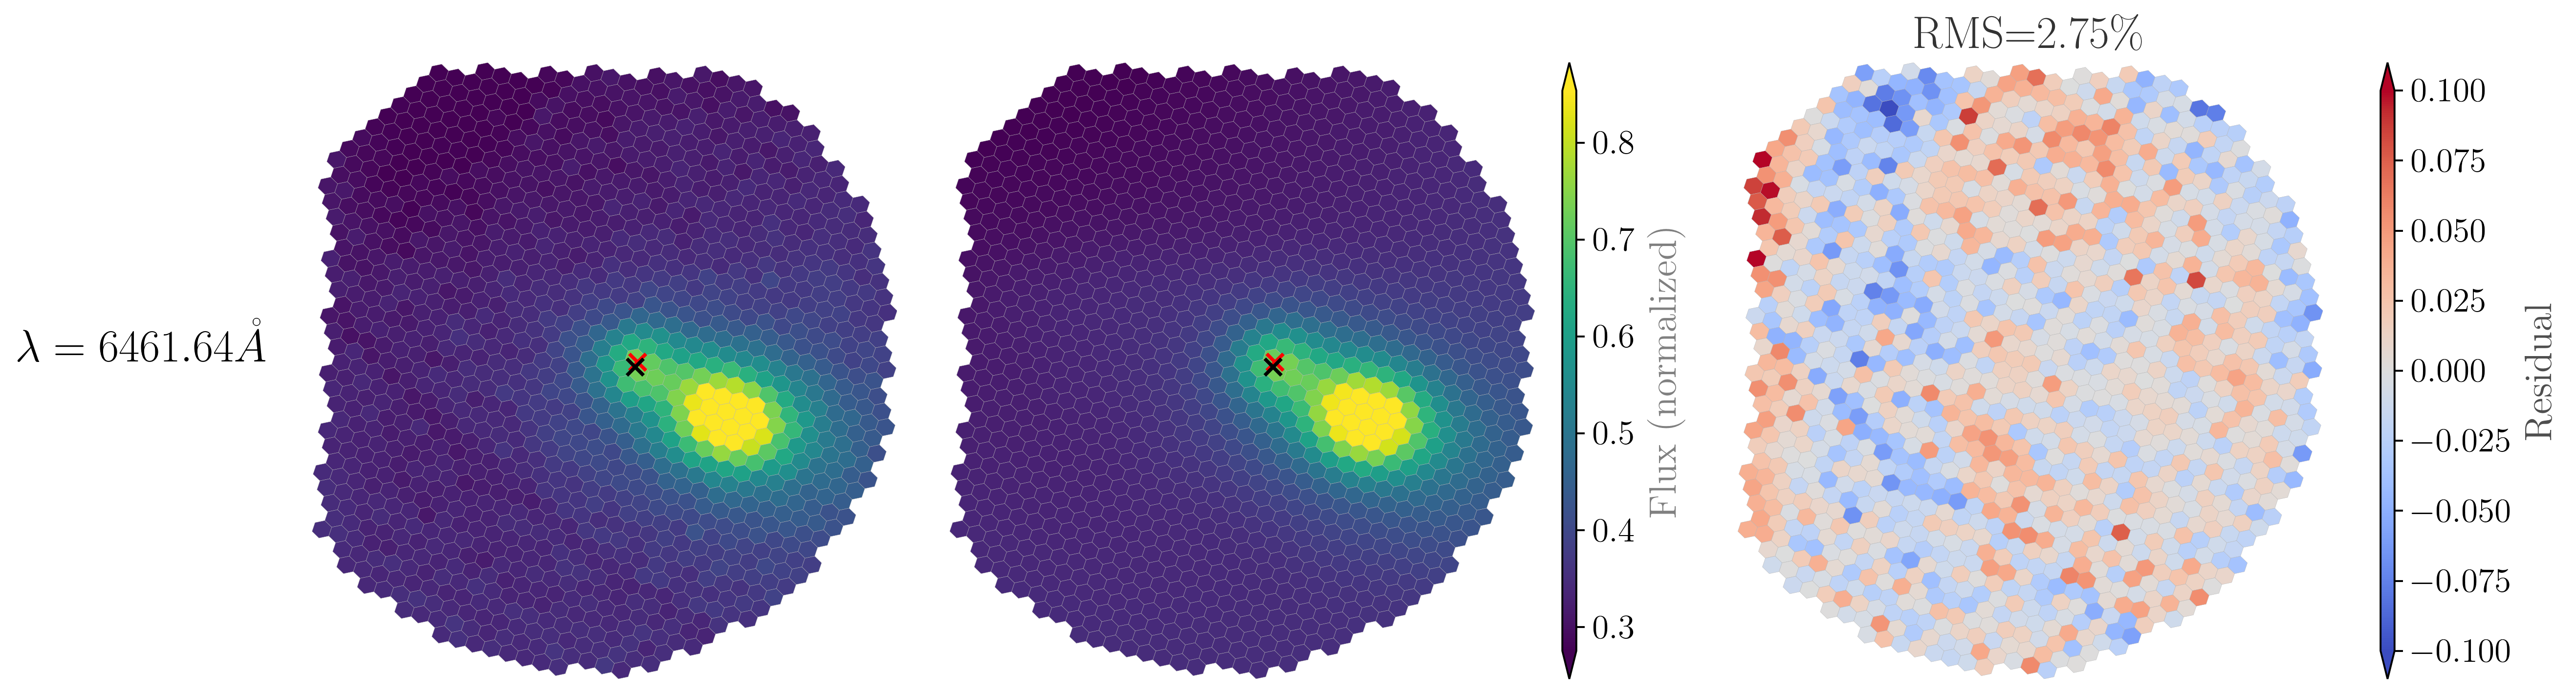
\includegraphics[width=0.8\textwidth]{../figures/07_scene/fitted_metasliceZTF18accrorf_2.png}
  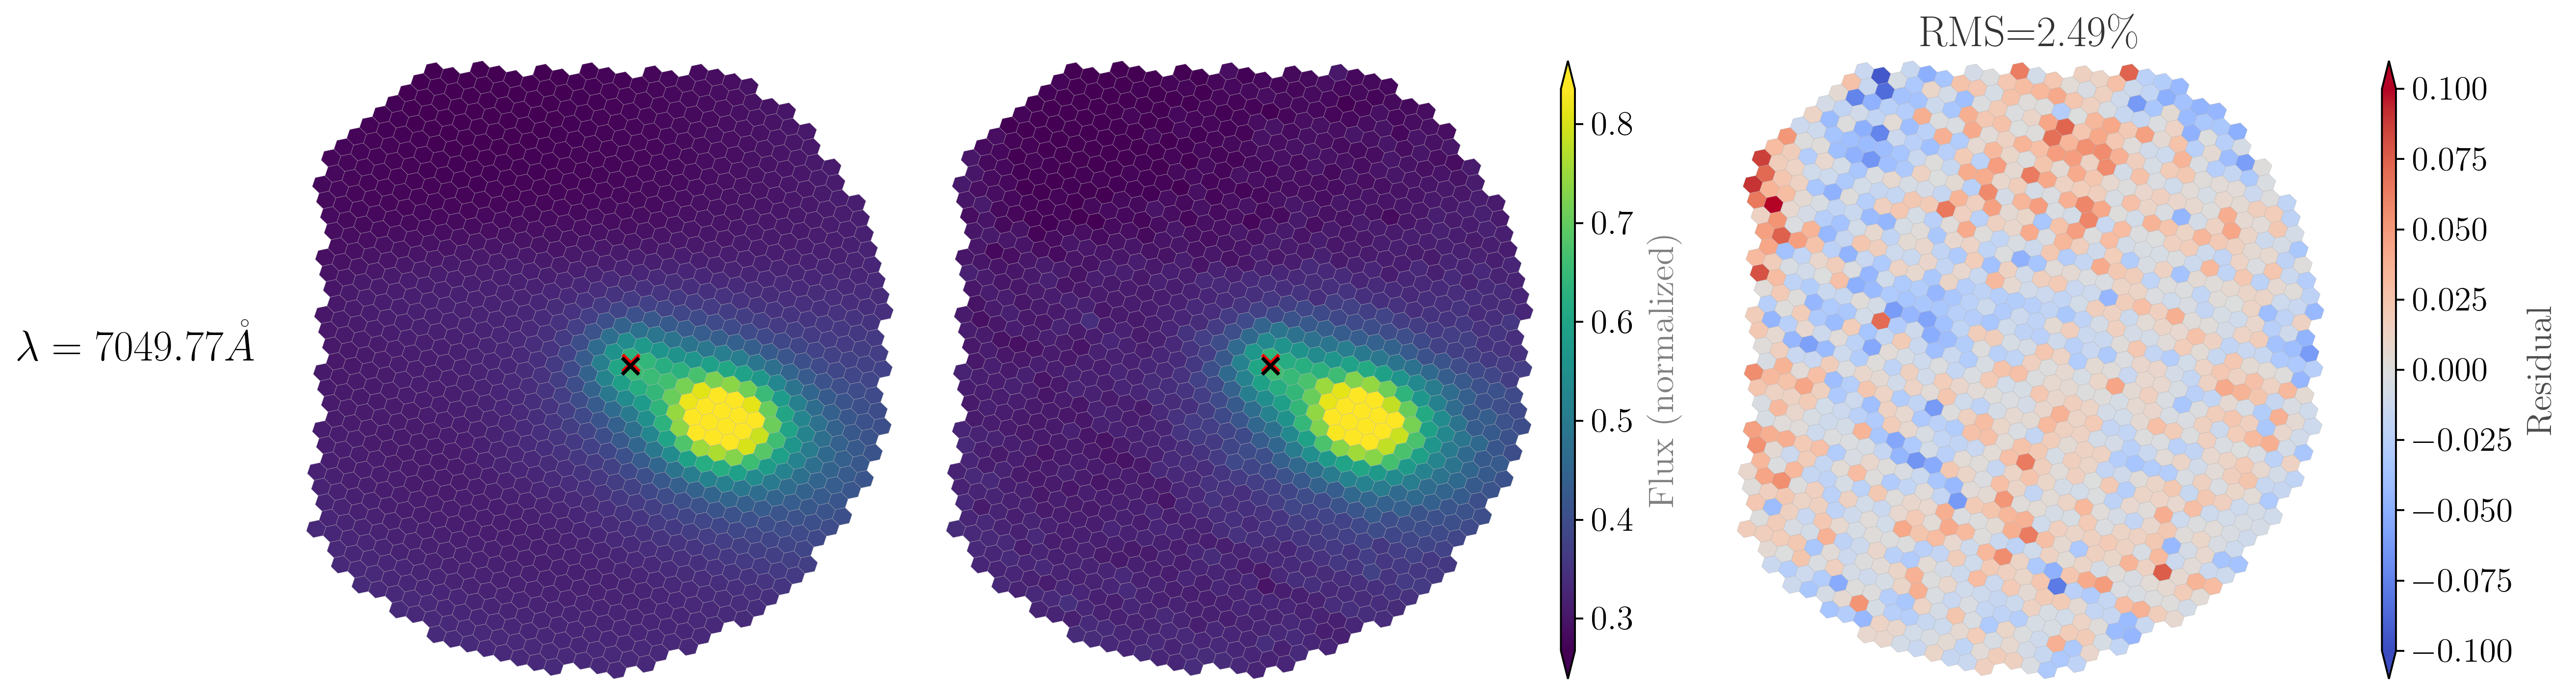
\includegraphics[width=0.8\textwidth]{../figures/07_scene/fitted_metasliceZTF18accrorf_3.png}
  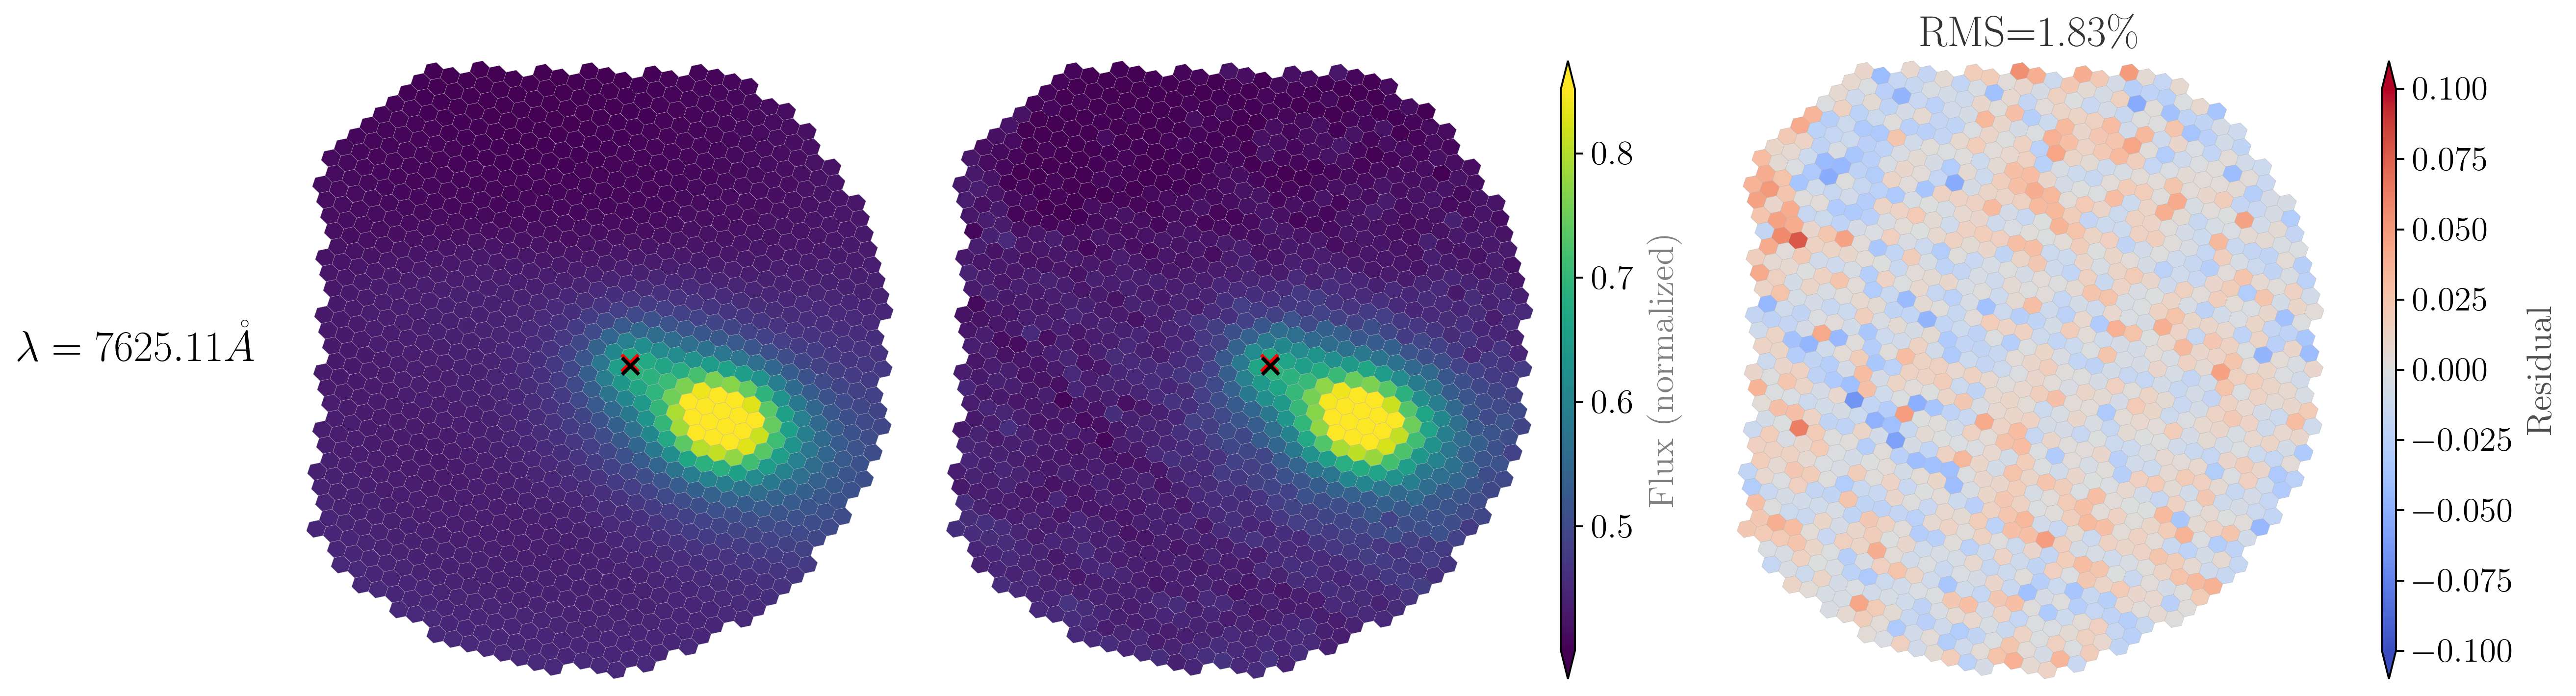
\includegraphics[width=0.8\textwidth]{../figures/07_scene/fitted_metasliceZTF18accrorf_4.png}
  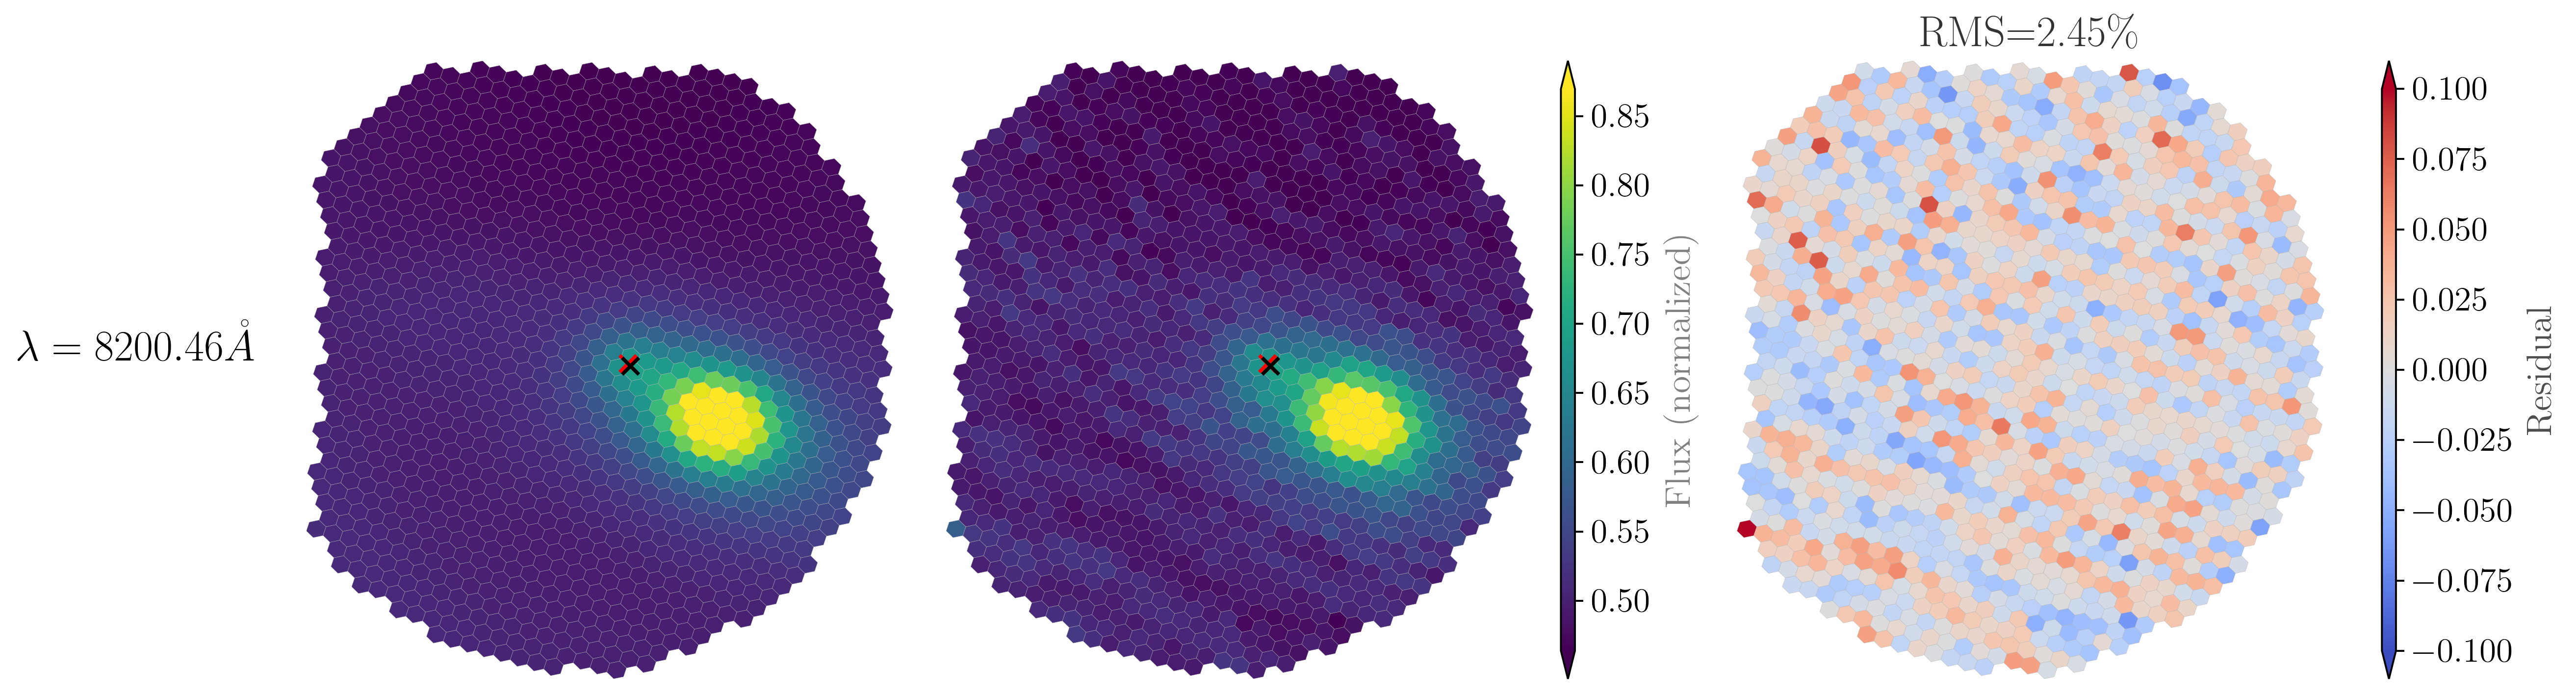
\includegraphics[width=0.8\textwidth]{../figures/07_scene/fitted_metasliceZTF18accrorf_5.png}
  \caption[Ajustement des méta-tranches pour la modélisation de scène de ZTF18accrorf.
  ]{Ajustement des méta-tranches pour la modélisation de scène de
    ZTF18accrorf. \emph{De haut en bas} sont représentées les
    méta-tranches modélisées du bleu vers le rouge. Pour chaque ligne
    \emph{de gauche à droite}: La méta-tranche modélisée par \hypergal,
    la méta-tranche du cube de données SEDm, et le résidu pondéré par le
  modèle. Nous indiquons pour chaque longueur d'onde le RMS spatial de
  l'ajustement, allant de $1.8\%$ à $3.9\%$. Les croix noires et rouges
  indiquent respectivement la position d'ancrage initiale (caméra de
  guidage), et la position ajustée par \hypergal.}
  \label{fig:metaslicescene}
\end{figure}

La Figure~\ref{fig:corrmatrixmetaslice} quant à elle présente la matrice
de corrélation entre les paramètres libres de la scène pour la
méta-tranche à $\lambda=6461$\AA.
\begin{figure}
  \centering
  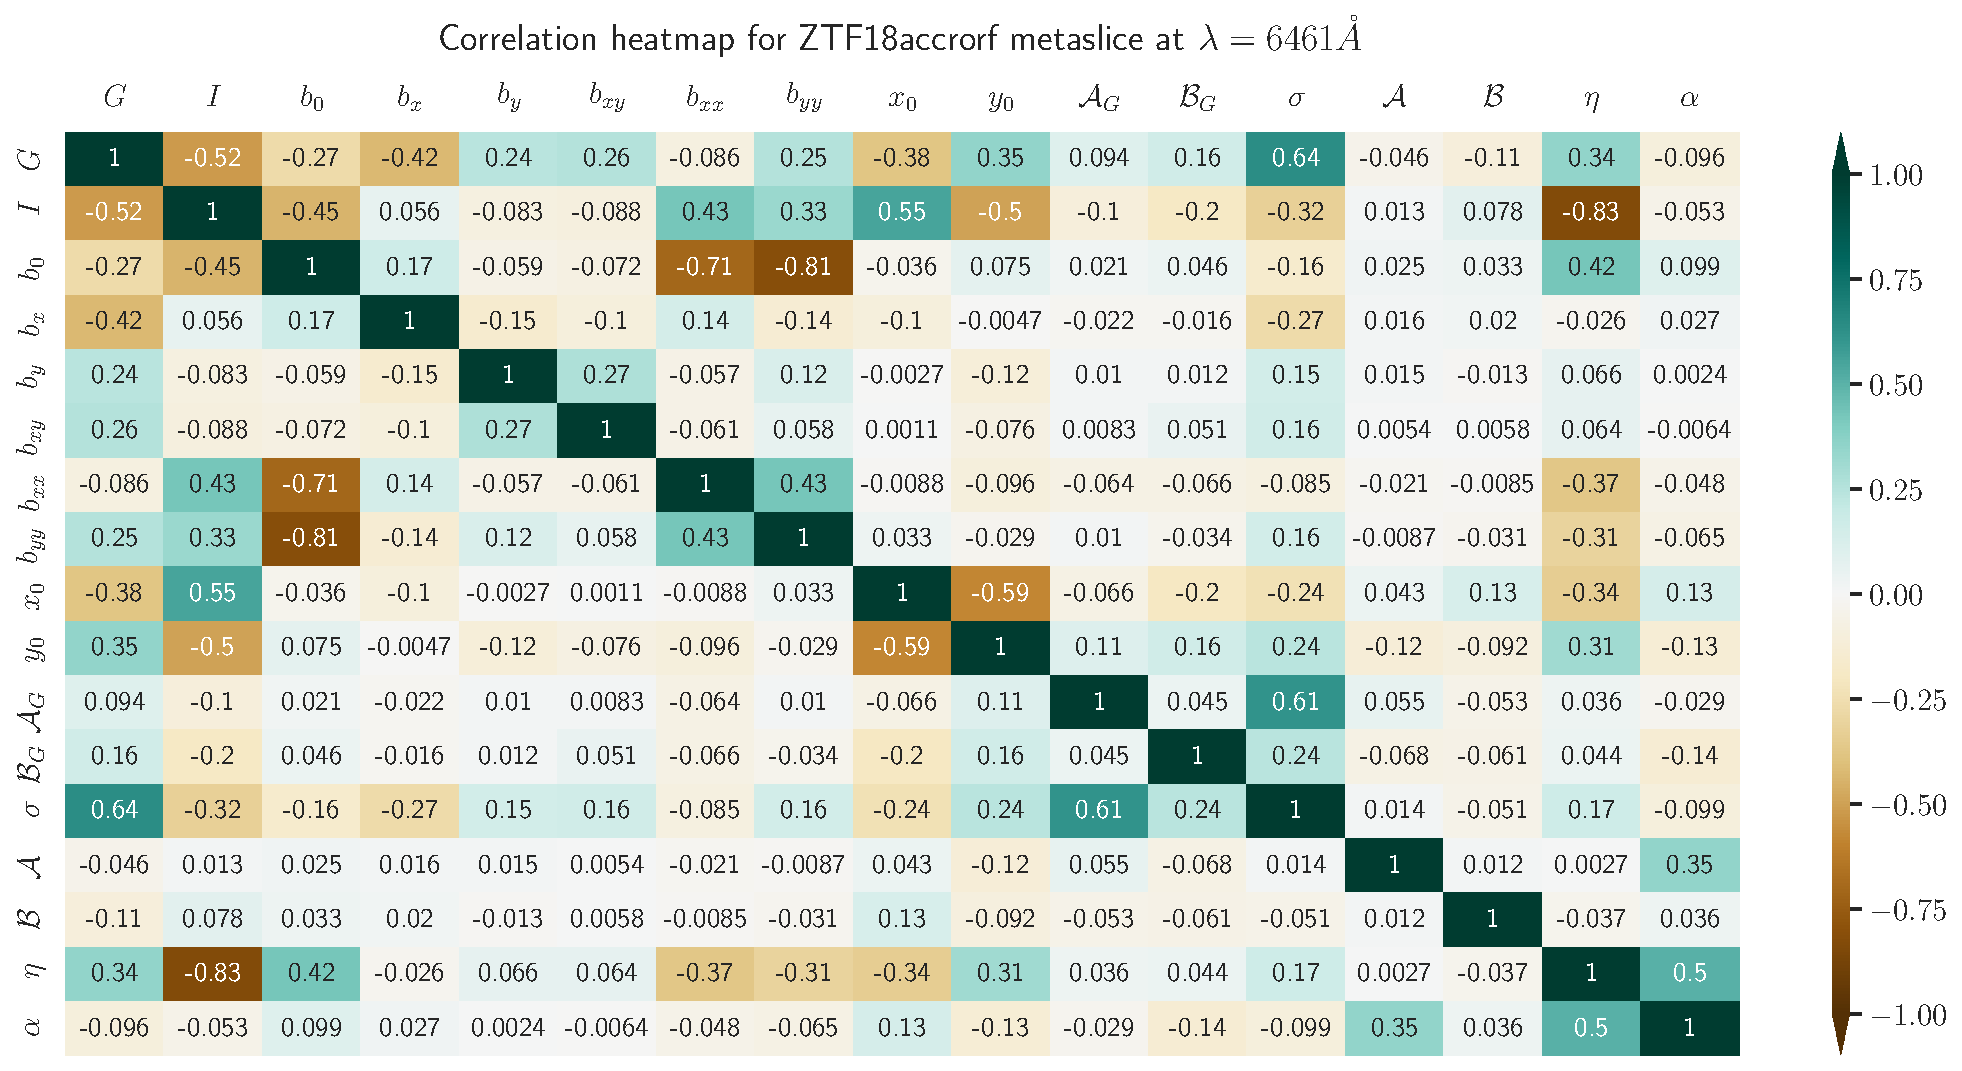
\includegraphics[width=0.95\textwidth]{../figures/07_scene/heatmapcorrelation_metaslice.pdf}
  \caption[Matrice de corrélation des paramètres d'ajustement de scène
  pour une méta-tranche.]{Matrice de corrélation des paramètres
    d'ajustement de scène de ZTF18accrorf pour la méta-tranche à $\lambda=6461$\AA.}
  \label{fig:corrmatrixmetaslice}
\end{figure}

\subsection{Ajustement chromatique}
% \label{ssec:xxx}
L'ajustement de chaque méta-tranche nous donne ainsi un jeu de $N$
paramètres sur le domaine spectral [$5000$,$8000$]\AA. Nous modélisons
la chromaticité de la PSF de la source ponctuelle de la même manière
qu'avec les étoiles standards: une loi de puissance pour $\alpha$ (rayon
de la Moffat), et
une constante pour $\eta$ (poids gaussienne/Moffat), $\mathcal{A}$ et
$\mathcal{B}$ (ellipticité et orientation).

Nous montrons dans la Figure~\ref{fig:chromaticity_target} la
modélisation chromatique de ces 4 paramètres. 

\begin{figure}[ht]
  \centering
  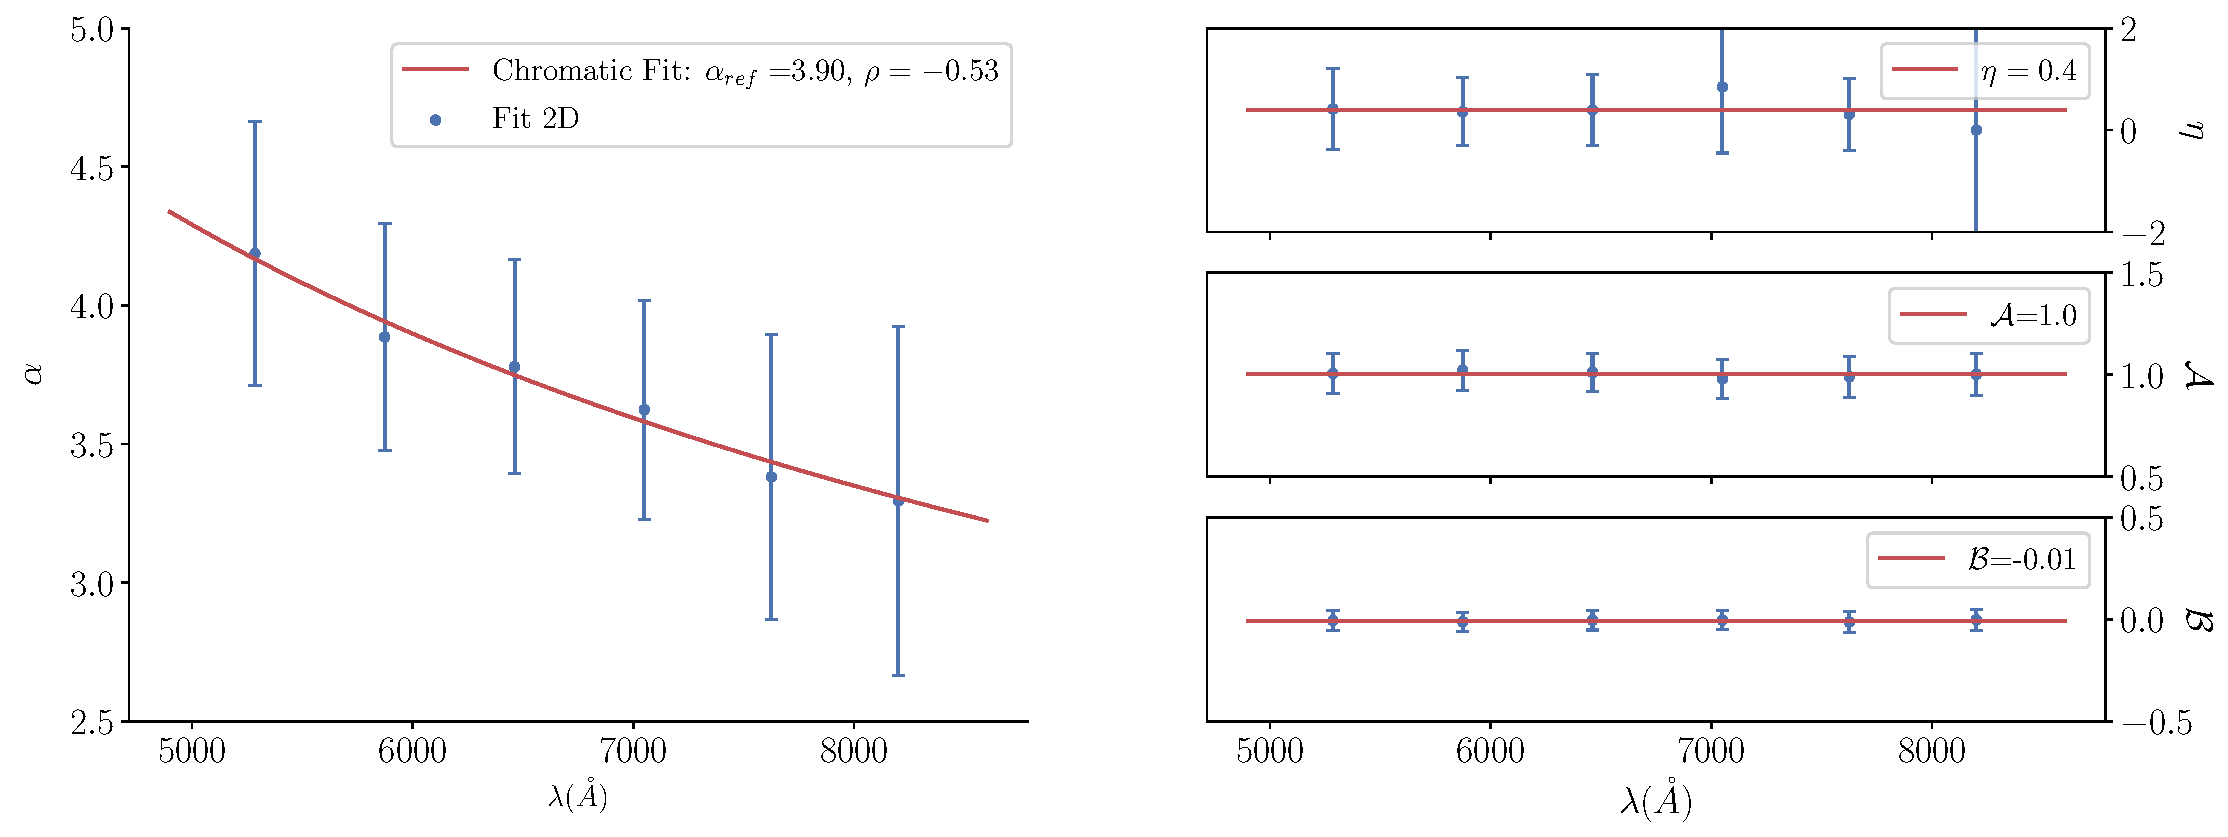
\includegraphics[width=0.78\textwidth]{../figures/07_scene/chromaticity_targetZTF18accrorf.pdf}
  \caption[Chromaticité des paramètres de forme de la PSF de la supernova ZTF18accrorf]{Ajustement de
    la chromaticité
    des paramètres de forme de la PSF pour la supernova ZTF18accrorf, à
    partir des 6 méta-tranches. \emph{À gauche} l'ajustement du paramètre $\alpha$ avec une
    loi de puissance. \emph{À droite} de haut en bas, l'ajustement par une
    constante de $\eta$ (poids entre la gaussienne et la Moffat) et des
    paramètres d'ellipticité ($\mathcal{A}$) et d'orientation ($\mathcal{B}$). }
  \label{fig:chromaticity_target}
\end{figure}

Nous utilisons également pour l'ellipticité et l'orientation de la PSF
relative (SEDm/PS1) une modélisation chromatique par une constante.

La chromaticité du rayon de la gaussienne de cette PSF relative est
modélisée par une loi de puissance, de la même façon que le paramètre de forme principal de la
source ponctuelle:
\begin{equation}
  \label{eq:sigmahostchrom}
  \sigma(\lambda)=\sigma_{ref}\left(\frac{\lambda}{\lambda_{ref}}\right)^{\rho_{g}}
\end{equation}

De la même façon que pour la source ponctuelle, nous montrons dans la Figure~\ref{fig:chromaticity_host} la
modélisation chromatique des paramètres décrivant la PSF relative par
laquelle nous avons convolué les méta-tranches du cube intrinsèque.

\begin{figure}[ht]
  \centering
  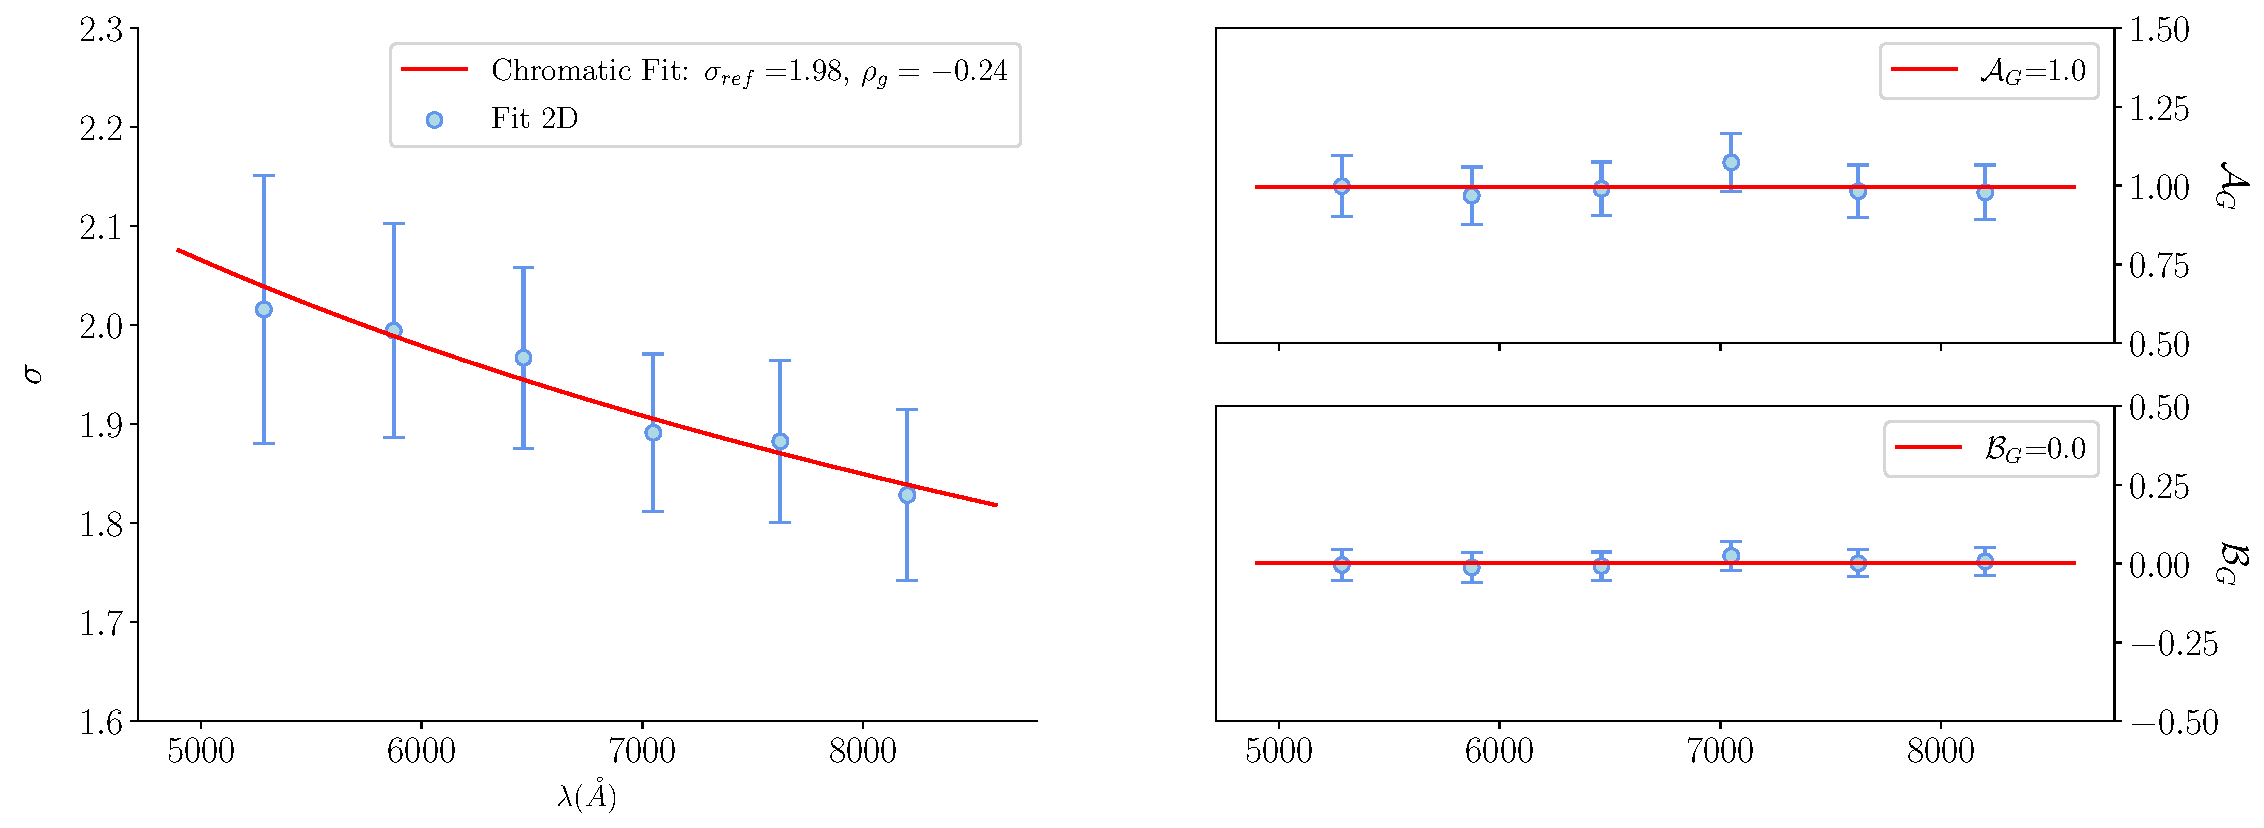
\includegraphics[width=0.78\textwidth]{../figures/07_scene/chromaticity_hostZTF18accrorf.pdf}
  \caption[Chromaticité des paramètres de forme de la PSF relative
  SEDm/PS1 pour l'hôte de ZTF18accrorf]{Ajustement de
    la chromaticité
    des paramètres de forme de la PSF relative SEDm/PS1 pour la galaxie
    hôte de la supernova ZTF18accrorf, à
    partir des 6 méta-tranches. \emph{À gauche} l'ajustement du paramètre $\sigma$ avec une
    loi de puissance. \emph{À droite} de haut en bas, les
    paramètres d'ellipticité ($\mathcal{A}_{G}$) et d'orientation ($\mathcal{B}_{G}$).}
  \label{fig:chromaticity_host}
\end{figure}

Enfin, à partir de l'ajustement de la position d'ancrage lors de la
projection pour chaque méta-tranche, nous modélisons les paramètres de la réfraction atmosphérique
différentielle pour cette observation. Cet ajustement est illustré dans
la Figure~\ref{fig:adr_ZTF18accrorf}.

\begin{figure}[ht]
  \centering
  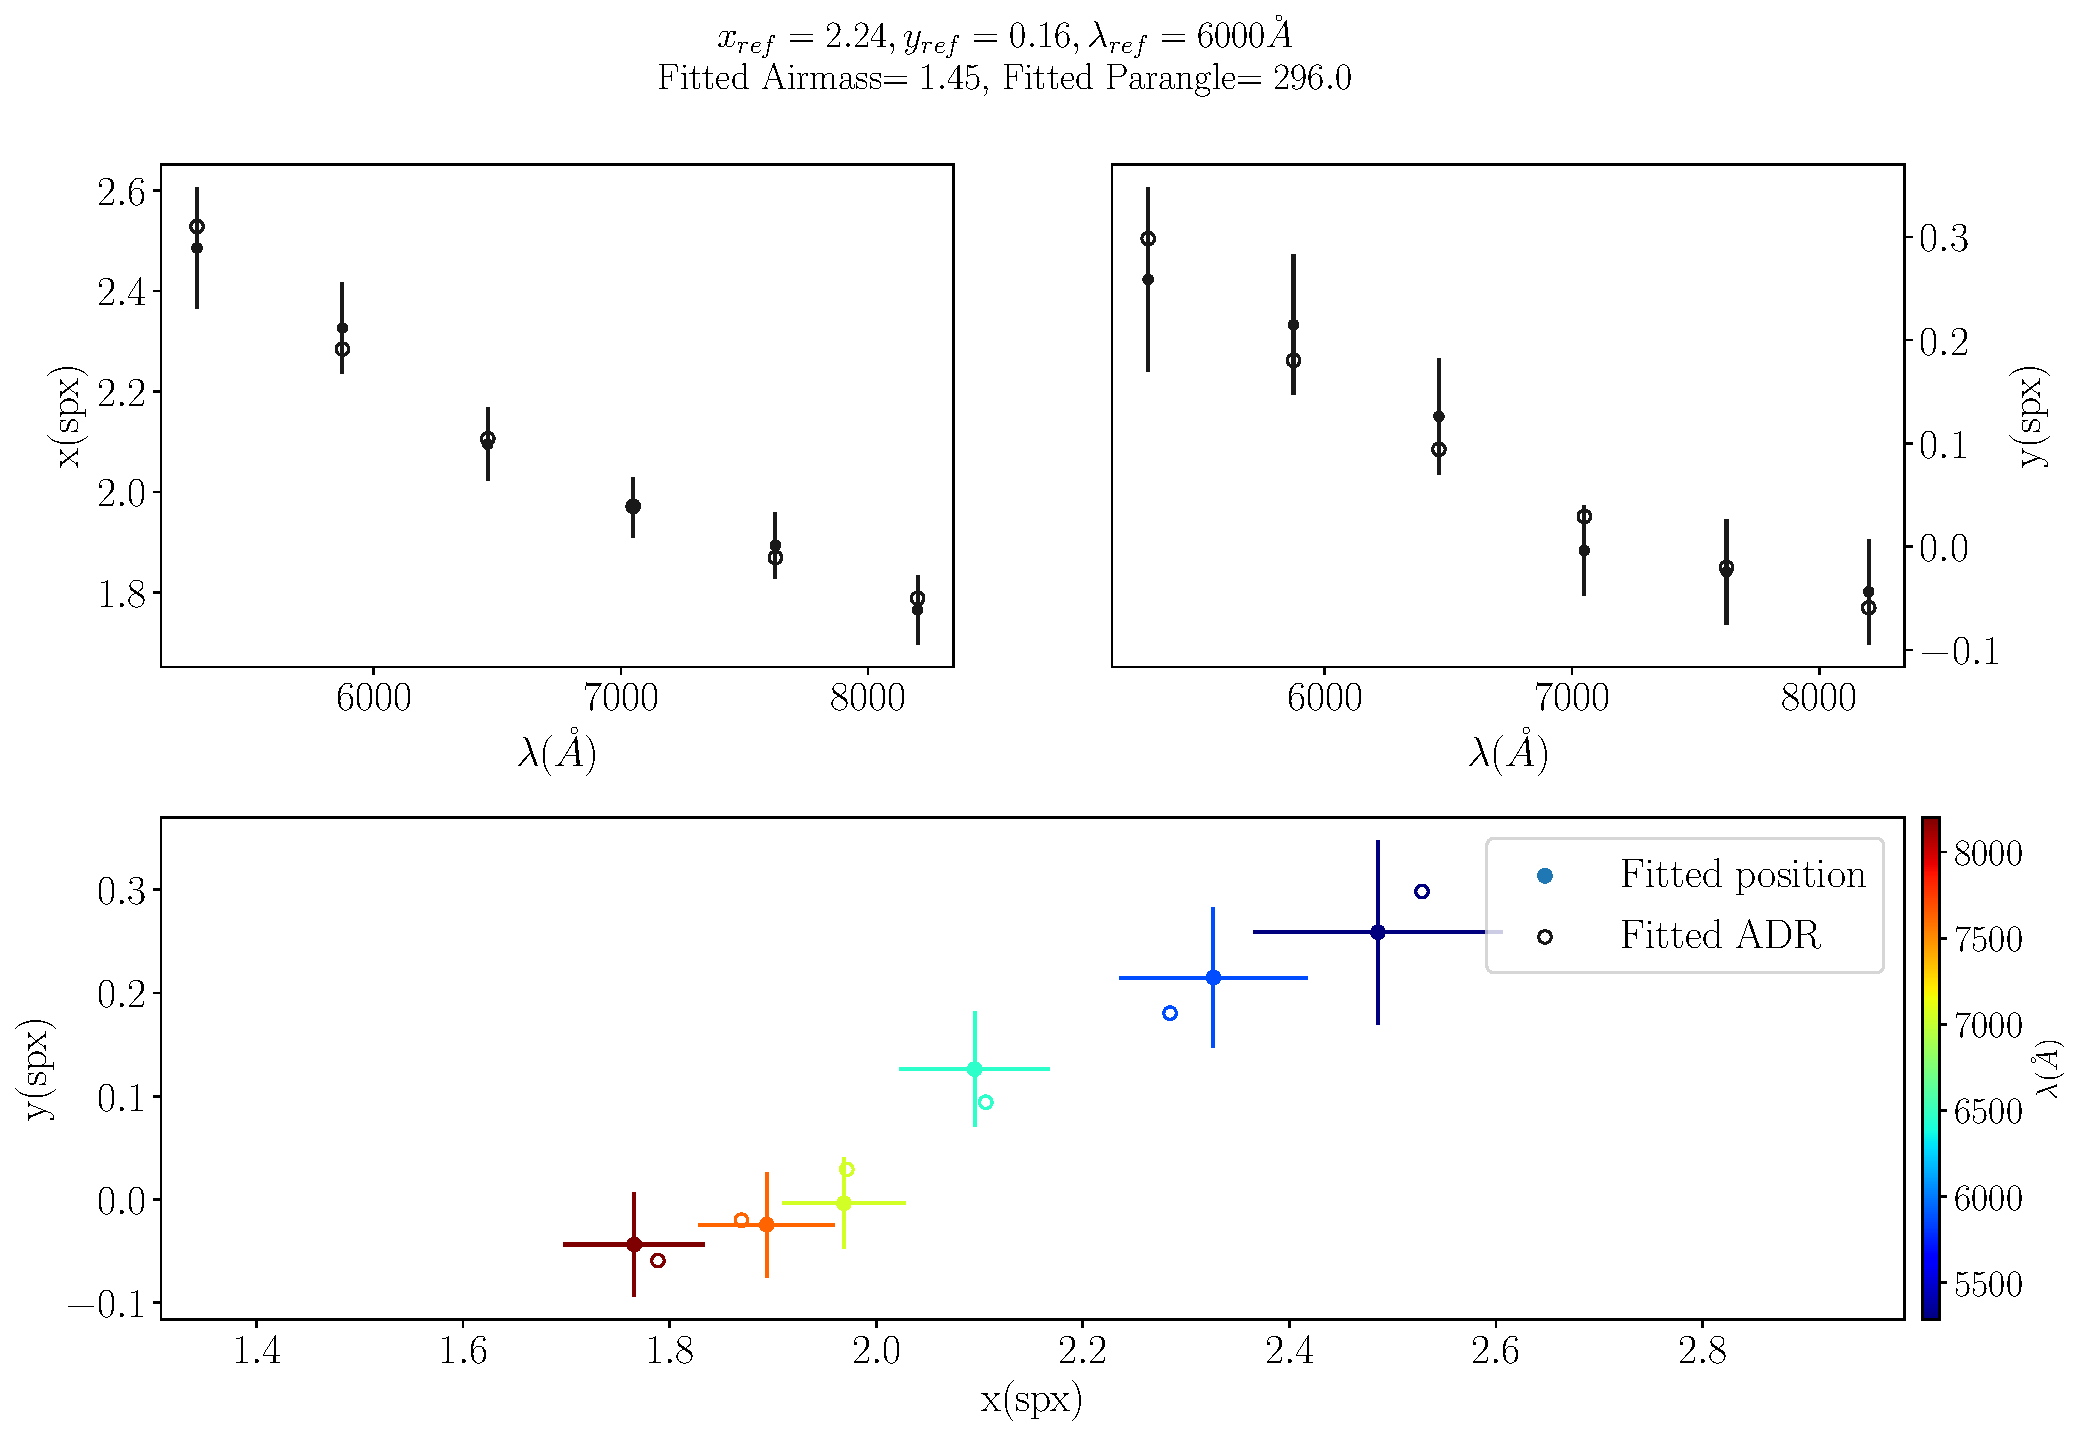
\includegraphics[width=0.78\textwidth]{../figures/07_scene/adr_ZTF18accrorf.pdf}
  \caption[Modélisation de la réfraction atmosphérique
  différentielle pour ZTF18accrorf]{Modélisation de la réfraction atmosphérique
    différentielle pour ZTF18accrorf. Nous montrons ici
    l'ajustement de la position d'ancrage ($x_{0}$,$y_{0}$) qui
    représente le centroïde de la supernova par le modèle
    d'ADR présenté dans le chapitre~\ref{ch:irf}. Les deux graphes du haut représentent l'ajustement des deux
    coordonnées en fonction de la longueur d'onde. Le graphe du bas
    illustre l'effet de la réfraction atmosphérique.}
  \label{fig:adr_ZTF18accrorf}
\end{figure}

Si pour une raison quelconque l'ajustement d'une méta-tranche n'a pas
convergé, celle-ci est ignorée lors de l'ajustement chromatique. D'autre
part, nous limitons l'impacte de potentielles valeurs aberrantes en
utilisant une fonction de perte de Huber \citep{Huber1964}. Plus
exactement, nous utilisons la fonction de perte \textit{pseudo-Huber}
d'ordre 1 (appelée \textit{soft-l1}),
qui est une approximation lisse de la fonction originale, définie elle par
morceau.
Si on considère comme l'analogie méchanique à un ajustement de
$\chi^{2}$ un système avec des forces attractives, alors les points de
données attirent le modèle avec une force possédant un potentiel $V(a)$
pour un décalage quadratique $a$. La Figure~\ref{fig:softl1} montre la
forme d'un potentiel standard (fonction de perte linéaire), en
comparaison avec un potentiel pseudo-Huber d'ordre 1. On voit que
l'utilisation de ce potentiel permet d'affaiblir le poids des valeurs
aberrantes, ce qui permet de ne pas faire dévier excessivement
l'ajustement du modèle.

\begin{figure}[ht]
  \centering
  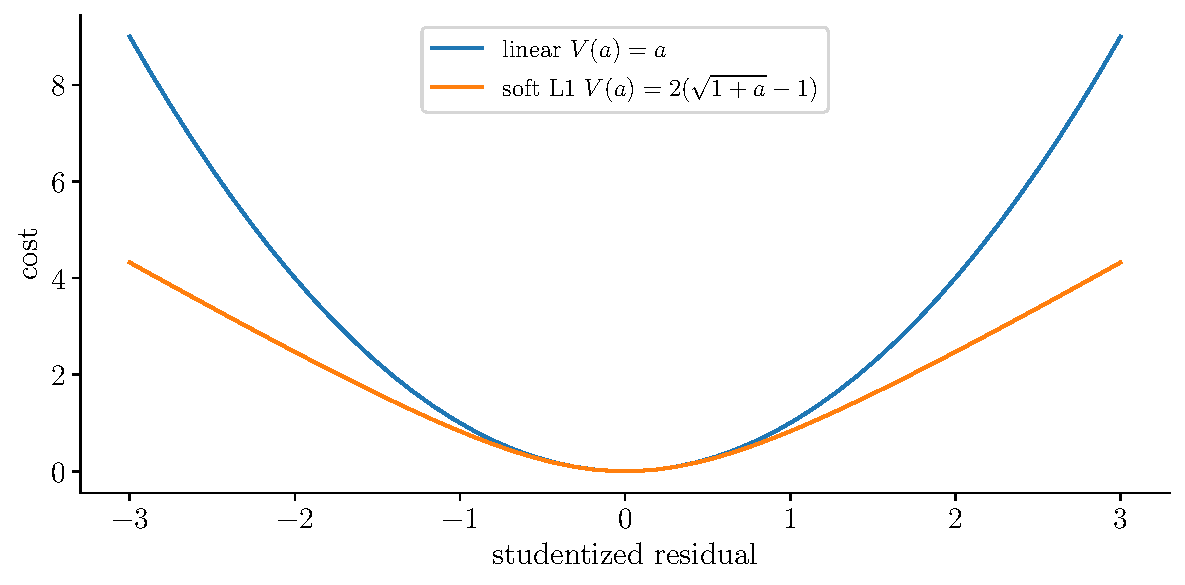
\includegraphics[width=0.6\textwidth]{../figures/07_scene/softl1.pdf}
  \caption[Fonction de perte \textit{pseudo-Huber}]{Mise en évidence du
    poids plus faible accordé aux valeurs aberrantes avec la fonction de perte \textit{pseudo-Huber}.}
  \label{fig:softl1}
\end{figure}

\begin{frshaded*}
  \footnotesize  
  \centerline{\emph{Estimation des valeurs initiales pour la modélisation
      de scène des méta-tranches.}}  
  Toute la procédure expliquée précédemment, de l'ajustement 2D des
  méta-tranches à l'ajustement chromatique, est également réalisée directement entre les images PS1 et les
  méta-tranches à transmission équivalentes du cube SEDm. Nous
  effectuons cette étape préliminaire simultanément
  avec la construction du cube intrinsèque afin d'optimiser le temps de
  calcul et les ressources numériques utilisées.
  Ces ajustements permettent d'obtenir un
  jeu de paramètres initial pour l'ajustement de scène principal.
\end{frshaded*}

Une fois l'ajustement de la chromaticité des paramètres de la scène
effectué, nous fixons tous les paramètres et procédons à l'ajustement
de toutes les tranches du cube en laissant libre les paramètres de
nuisances. Le coefficient d'amplitude correctif de la galaxie $G$ et
également laissé libre pour toutes les tranches. Nous avons remarqué que cela
permet de prévenir les
potentiels sur/sous-estimations de l'intensité des raies modélisées dans
le cube intrinsèque, d'éventuels fluctuations causées par une
calibration en flux de mauvaise qualité ou encore des résidus
telluriques dans le cube SEDm. Nous reviendrons sur ce point à la fin de
cette section lors de l'extraction des sources pour illustrer nos propos.

La Figure~\ref{fig:fullsceneZTF18accrorf} montre le résultat final de la
modélisation de scène effectuée avec \hypergal\ pour la supernova
ZTF18accrorf. Nous y présentons l'image 2D du cube de données SEDm et du cube
modélisé empilés entre $5000$\AA\ et $8500$\AA. Afin de contrôler la
qualité de l'ajustement, nous montrons également le pull spectral et le
RMS spectral pour chaque spaxel.

Le RMS spectral est calculé comme dans l'équation~\ref{eq:rms}. Le
pull spectral est quant à lui calculé après intégration du spectre pour
un spaxel donné de la façon suivante:

\begin{equation}
  \label{eq:pullspectral}
  p_{spx}=\frac{\sum\limits_{\lambda}\left( y_{\lambda}-\widetilde{y}_{\lambda}\right)}{\sqrt{\sum\limits_{\lambda}\sigma_{\lambda}^{2}}}
\end{equation}
avec $\widetilde{y}$ la prédiction du modèle, $y$ la donnée dans le cube
SEDm et $\sigma$ l'erreur sur $y$.

\begin{figure}
  \centering
  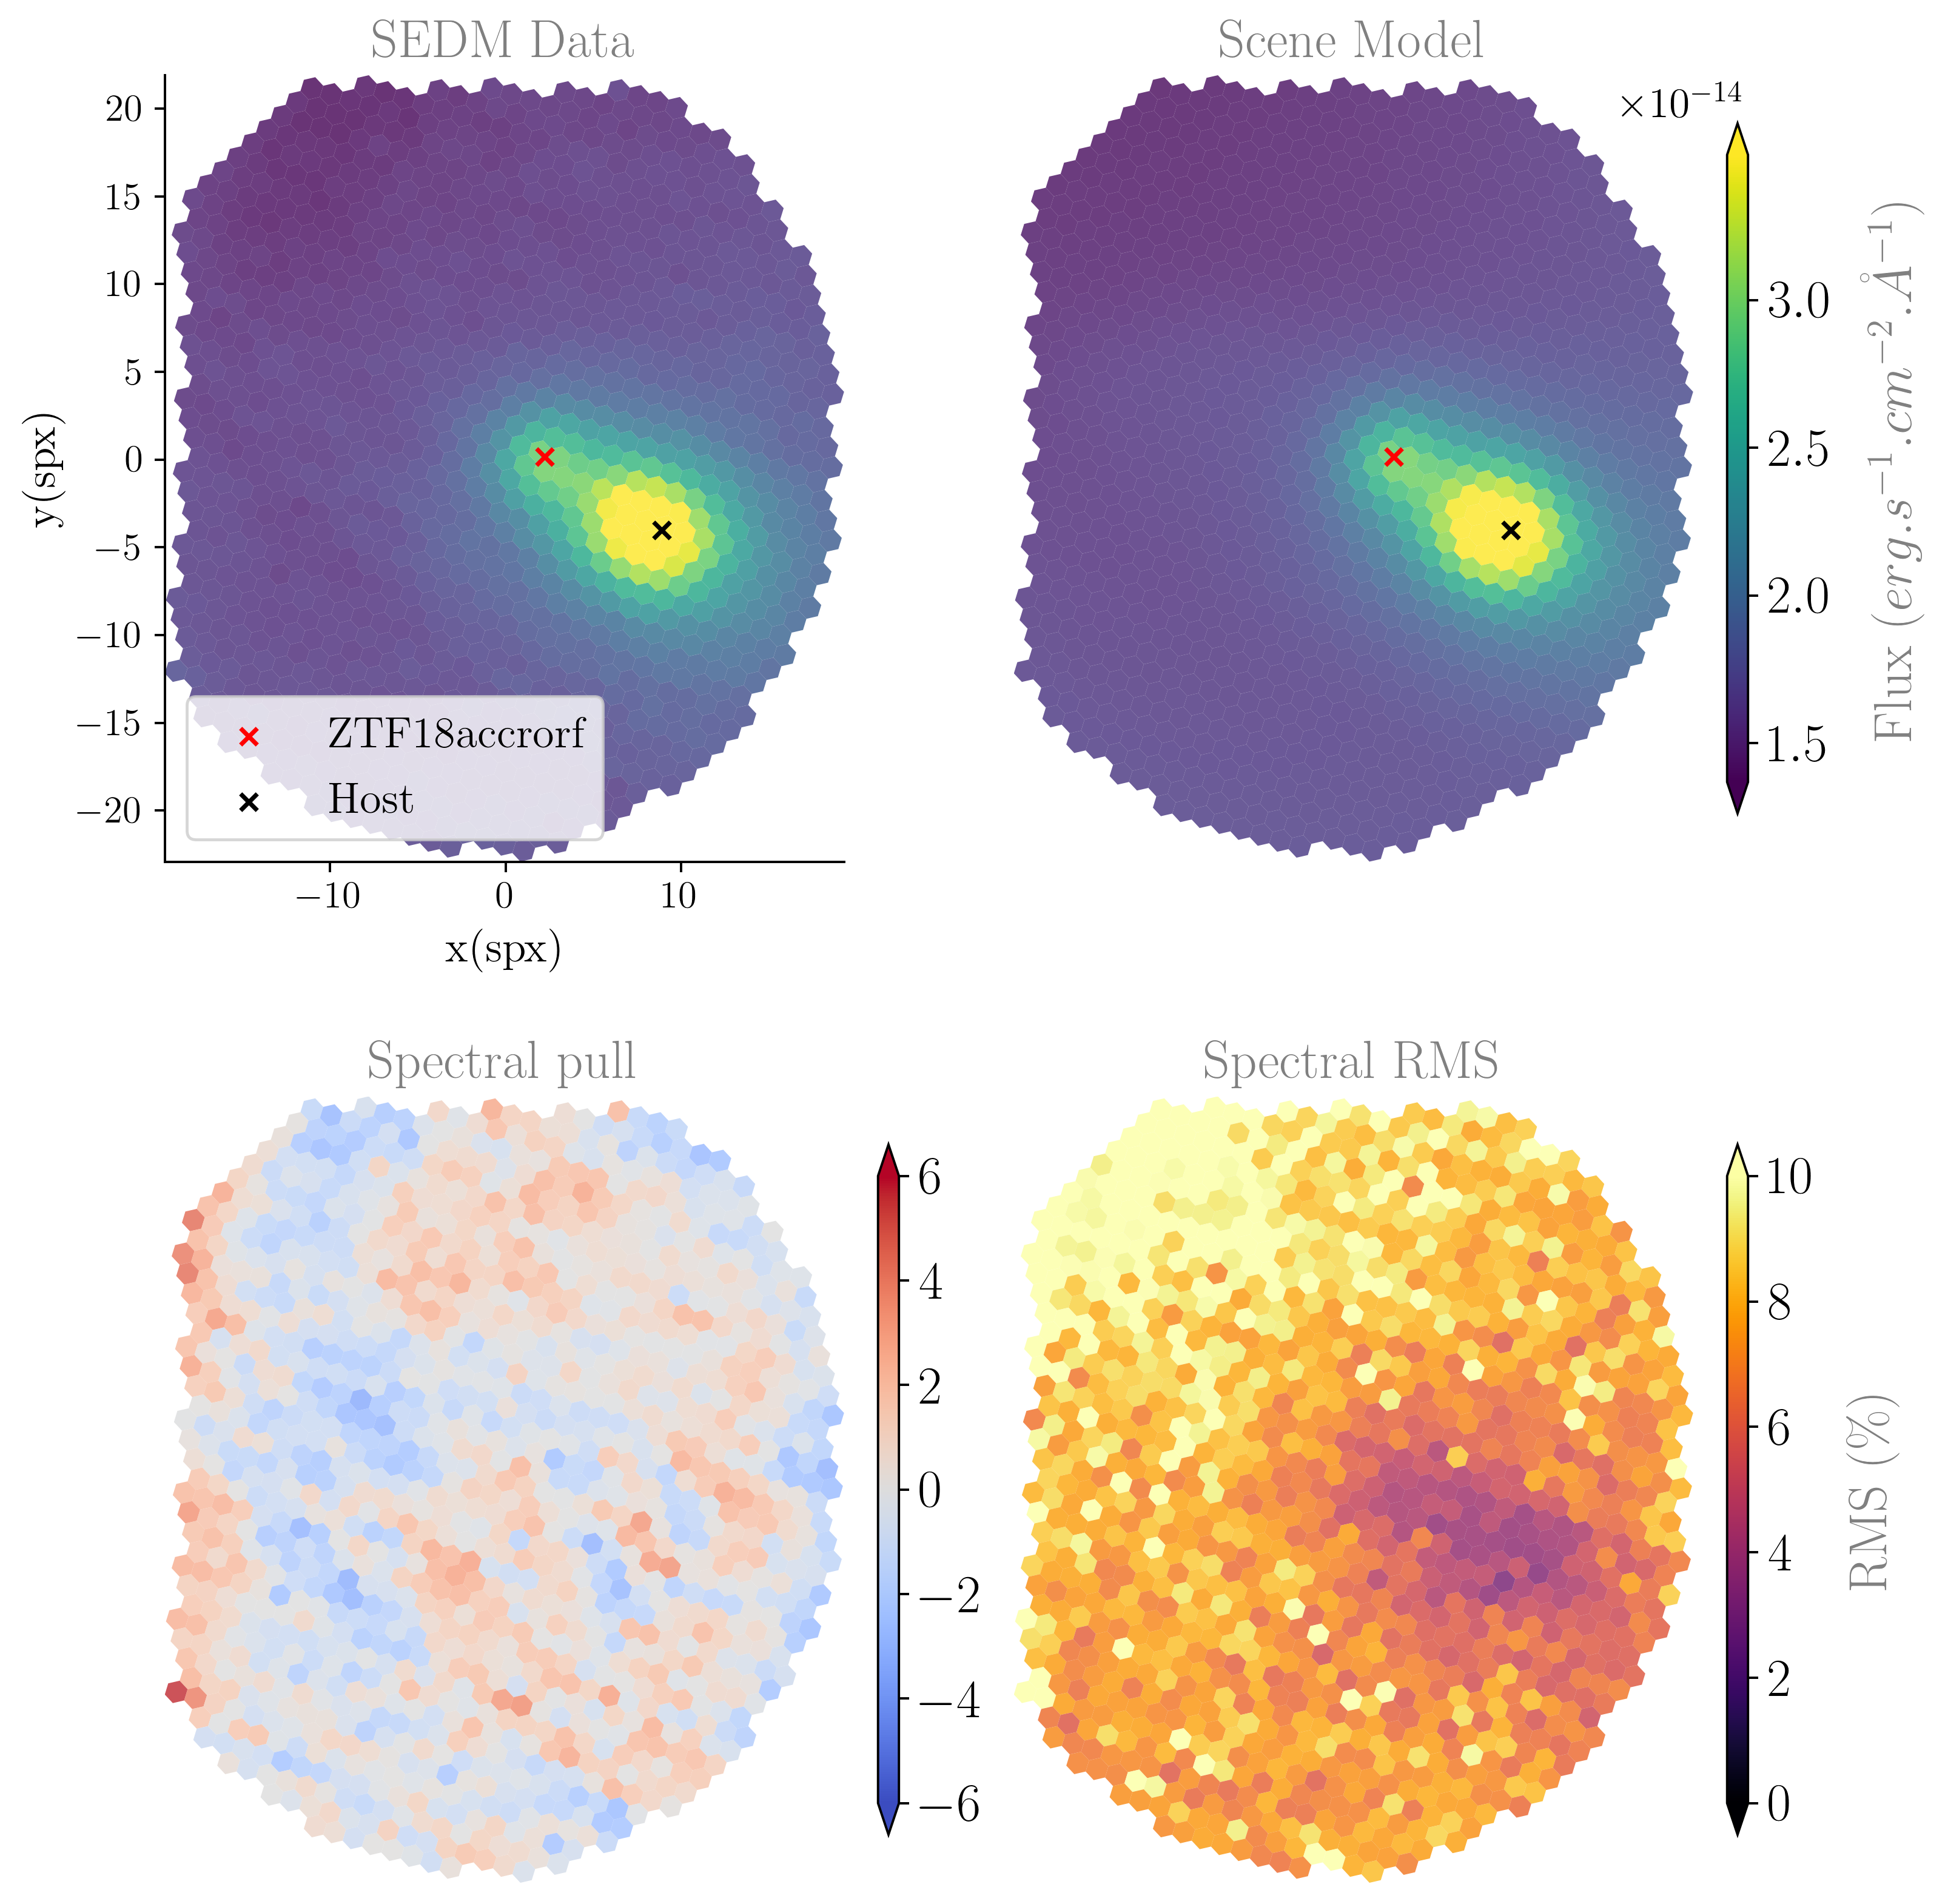
\includegraphics[width=0.8\textwidth]{../figures/07_scene/scene_rmspull_ZTF18accrorf.png}
  \caption[Modélisation de scène complète pour
  ZTF18accrorf.]{Modélisation de scène complète pour
    ZTF18accrorf. \emph{En haut} nous montrons \emph{de gauche à droite}:
  le cube de données SEDm empilé entre $5000$ et $8500$, puis le cube
  modélisé par \hypergal\ empilé également sur le même domaine
  spectral. La croix rouge indique la position ajustée de ZTF18accrorf à
$7000$\AA, et la croix noire la position de la galaxie hôte. \emph{En
  bas} nous montrons \emph{de gauche à droite}: le pull spectral tel que
définit dans l'équation~\ref{eq:pullspectral}, et le RMS spectral en
\%. Le pull nous permet de contrôler la présence éventuelle de structures dans le
résidu, ce qui n'est pas le cas ici. Le RMS quant à lui nous indique une
précision de l'ordre de $4\%$ sur le domaine spectral considéré au
niveau des sources présentes dans le champ de vue de la SEDm. Les
fluctuations du fond induisent un RMS spectral de l'ordre de $6$-$7\%$,
et nous pouvons clairement voir les conséquences de l'artefact en haut à
gauche du cube de données.}
  \label{fig:fullsceneZTF18accrorf}
\end{figure}

\section{Extraction des sources}

Une fois la modélisation de scène complétée, résultant en
un cube 3D dans l'espace des observations de la SEDm, nous sommes en mesure
d'extraire chacune des composantes: le fond, la galaxie hôte et la source
ponctuelle. 

\subsection{Extraction de la galaxie hôte}\label{ssec:hostextract}

Afin d'extraire la galaxie hôte du cube de données, nous l'isolons en
soustrayant les modèles de fond et de la source ponctuelle au cube SEDm.

Une galaxie n'étant pas une source ponctuelle, nous devons
définir une ouverture afin d'en extraire le spectre.

Nous utilisons pour cela l'outil \pkg{sep}\footnote{\url{http://github.com/kbarbary/sep}}
\citep{Barbary2016Sep} (implémentation python de \pkg{Sextractor}
\cite{Bertinsextractor}), en définissant une ellipse d'ouverture dans
les images PS1 que nous
projetons ensuite dans le MLA de la SEDm à l'aide des
solutions WCS des deux espaces. Nous négligeons
les effets d'ADR dans cette procédure, étant donné qu'ils induisent rarement un déplacement de plus d'un
spaxel dans le champ de vue. Nous illustrons dans la
Figure~\ref{fig:hostspecZTF18accrorf} l'extraction du spectre de la
galaxie hôte de ZTF18accrorf, en considérant les spaxels mis en
évidences sur l'image du cube empilée. Ce que nous montrons ici n'est
pas le spectre de la galaxie modélisée, mais bien celui de la galaxie
dans le cube de données de la SEDm, auquel nous avons retiré les modèles
de fond et de la source ponctuelle.

De la même façon que la modélisation
hyperspectrale de la galaxie (et du fond) nous permet de lever la
contamination de la supernova, la modélisation de la supernova nous
permet également de réduire la contamination de la galaxie et de
l'isoler dans les cubes d'observation.

Connaissant également a priori le redshift utilisé pour la modélisation
de la galaxie, nous indiquons la position déduite de quelques raies
d'absorption et
d'émission\footnote{\url{http://astronomy.nmsu.edu/drewski/tableofemissionlines.html}}\footnote{\url{http://classic.sdss.org/dr6/algorithms/linestable.html}}
dans l'air \citep{Morton1991}, afin de visualiser la cohérence entre le
spectre isolé dans les données et le redshift utilisé. Dans le cas de
cette galaxie, nous pouvons par exemple voir la concordance entre le redshift
$z=0.042$ et la position de la raie H$\alpha$.

\begin{figure}[ht]
  \centering
  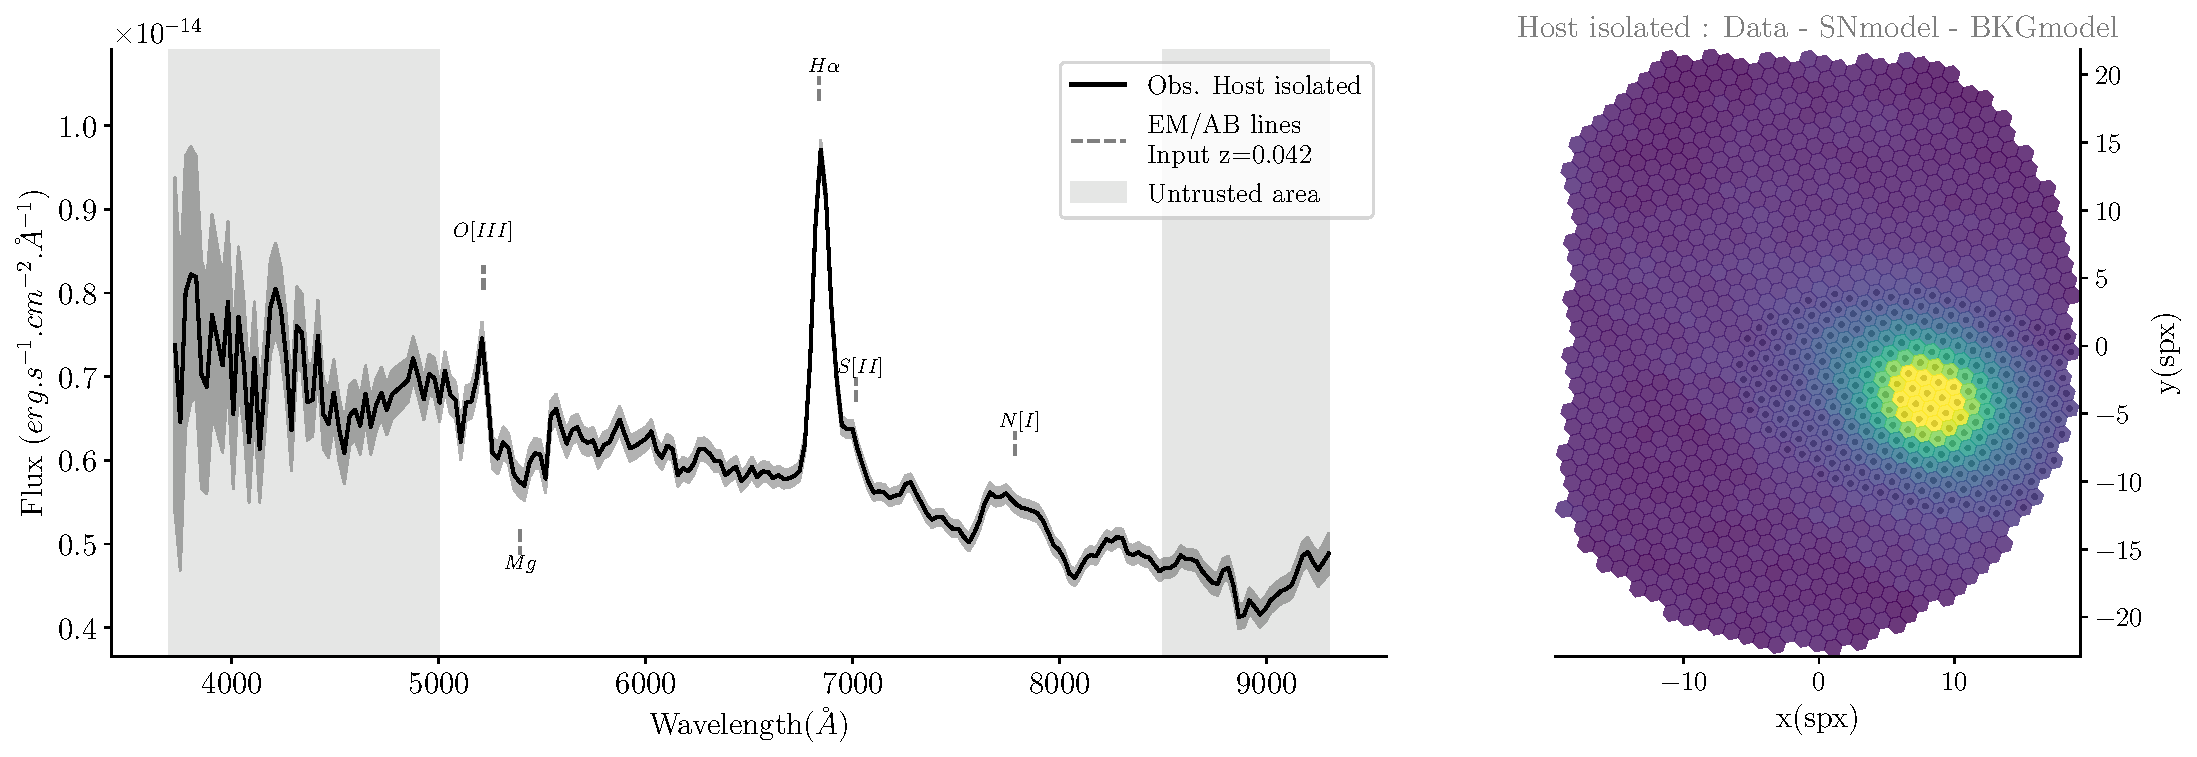
\includegraphics[width=0.9\textwidth]{../figures/07_scene/output_host_ZTF18accrorf.pdf}
  \caption[Extraction du spectre de la galaxie hôte de
  ZTF18accrorf]{Extraction du spectre de la galaxie hôte de
    ZTF18accrorf. \emph{À droite} nous montrons le cube de données de la
  SEDm, auquel nous avons soustrait les modèles de fond et de la source
  ponctuelle afin d'isoler la galaxie hôte. Les spaxels sélectionnés par
les losanges noirs indiquent ceux appartenant à l'ouverture utilisée
pour l'extraction du spectre. \emph{À gauche} nous montrons donc le
spectre extrait et l'erreur associée contenus dans cette ouverture. Tout le domaine spectral
de la SEDm est affiché, et les bandes grises indiquent les zones
auxquelles nous accordons généralement une faible fiabilité ($\lambda<5000$\AA\ et
$\lambda>8500$\AA) due aux artefacts
présents dans les cubes SEDm. Nous montrons également la position
théorique de quelques raies d'émission et d'absorption sachant le
redshift utilisé, et nous pouvons voir ici la bonne cohérence avec le
spectre extrait.}
  \label{fig:hostspecZTF18accrorf}
\end{figure}

\subsection{Extraction de la Supernova}\label{ssec:snextraction}

De la même façon qu'avec la galaxie hôte, nous pouvons vérifier la
l'isolation de la supernova dans le cube de données en y soustrayant le
modèle de fond et de la galaxie. La
Figure~\ref{fig:targetisolatedZTF18accrorf} illustre ainsi le cube SEDm
de l'observation auquel nous avons retiré les deux autres composantes,
et nous pouvons voir à quel point la supernova est bien définie sans
structure résiduelle apparente. Nous pouvons par exemple définir une
ouverture arbitraire (ici circulaire de $8$ spaxels $\sim4\farcs5$ de
rayon) centrée sur la position de la source ponctuelle et porter un
visuel sur le pull et le RMS spectral dans cette ouverture. Pour cette
observation nous pouvons par exemple voir un RMS spectral de l'ordre de
$3$-$4\%$ au niveau de la position de la supernova dans le cube, et
aucune structure résiduelle apparente (en provenance d'une mauvaise
modélisation galactique par exemple).

\begin{figure}
  \centering
  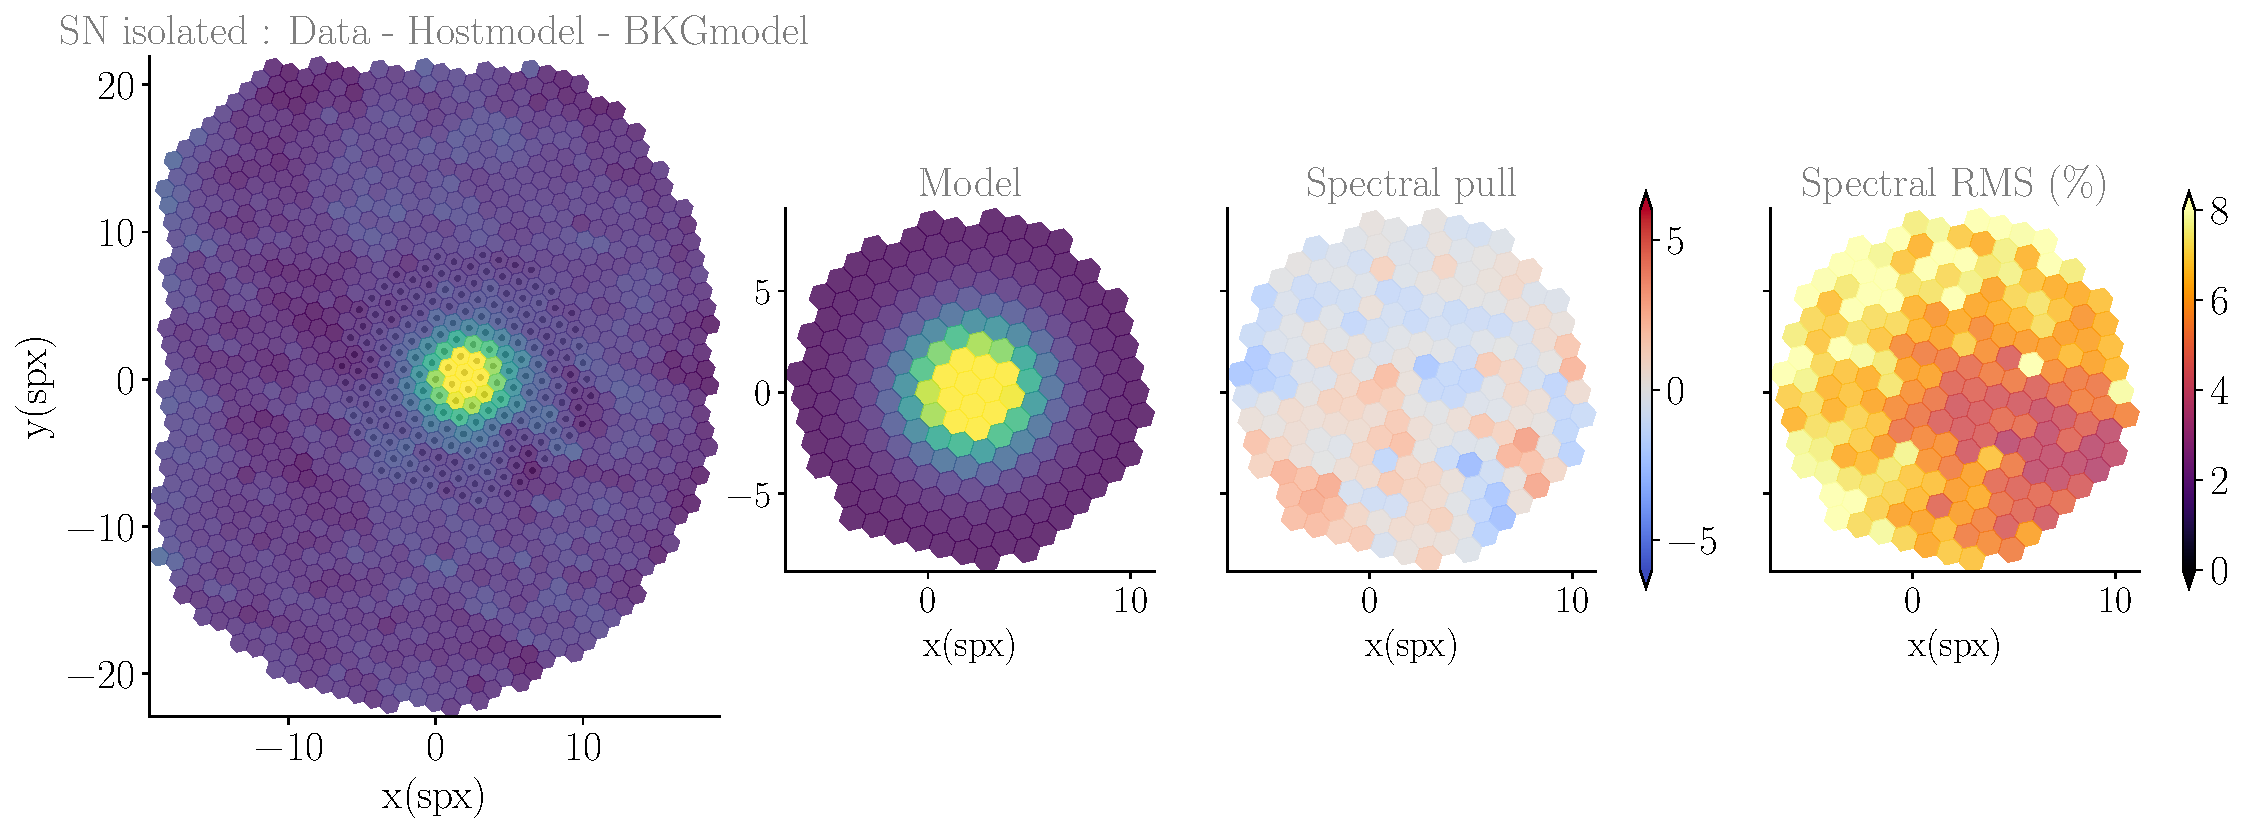
\includegraphics[width=0.99\textwidth]{../figures/07_scene/output_sn_ifu_ZTF18accrorf.pdf}
  \caption[Isolation de la supernova ZTF18accrorf dans le cube
  SEDm.]{Isolation de la supernova ZTF18accrorf dans le cube
    SEDm. Chaque image de cube 3D correspond à un empilement entre
    $5000$ et $8500$\AA. \emph{De gauche à droite}: (a) le cube de données SEDm auquel
    nous avons soustrait le modèle de la galaxie et celui du fond, ce
    qui met en évidence la qualité d'isolation de la supernova et à
    fortiori la qualité de modélisation des deux autres composantes. (b)
  Le cube modèle de la source ponctuelle limité à une ouverture
  circulaire de $8$ spaxels ($\sim4\farcs5$) de
rayon, définie par les spaxels mis en évidence dans (a) par les losanges
noirs. (c) Le pull spectral et (d) le RMS spectral dans cette ouverture,
tout deux définis comme dans la
Figure~\ref{fig:fullsceneZTF18accrorf}. Nous pouvons voir ici l'absence
de structure résiduelle, et un RMS spectral de l'ordre de $3$-$4\%$ au niveau de la position de ZTF18accrorf.}
  \label{fig:targetisolatedZTF18accrorf}
\end{figure}

Nous pouvons également vérifier la robustesse du modèle de PSF que nous
avons défini et contraint dans le chapitre précédent en superposant le
modèle ajusté de profil radial aux données. Afin de permettre également
un contrôle de la qualité de l'ajustement du fond de ciel, et la
présence éventuelle de structure résiduelle, nous visualisons ce profil
radial après soustraction du fond ajusté et du modèle hyperspectral de
la galaxie hôte. Nous montrons ainsi dans la
Figure~\ref{fig:radialprofileZTF18accrorf} le profil radial ajusté pour
une des méta-tranches. Nous pouvons voir que le fond de ciel tend bien
vers $0$, ce qui indique une bonne estimation de cette composante. Par
ailleurs, nous n'observons pas de valeur aberrante dans la supernova
isolée, ce qui à son tour traduit une soustraction galactique sans
résidu notable.

\begin{figure}
  \centering
  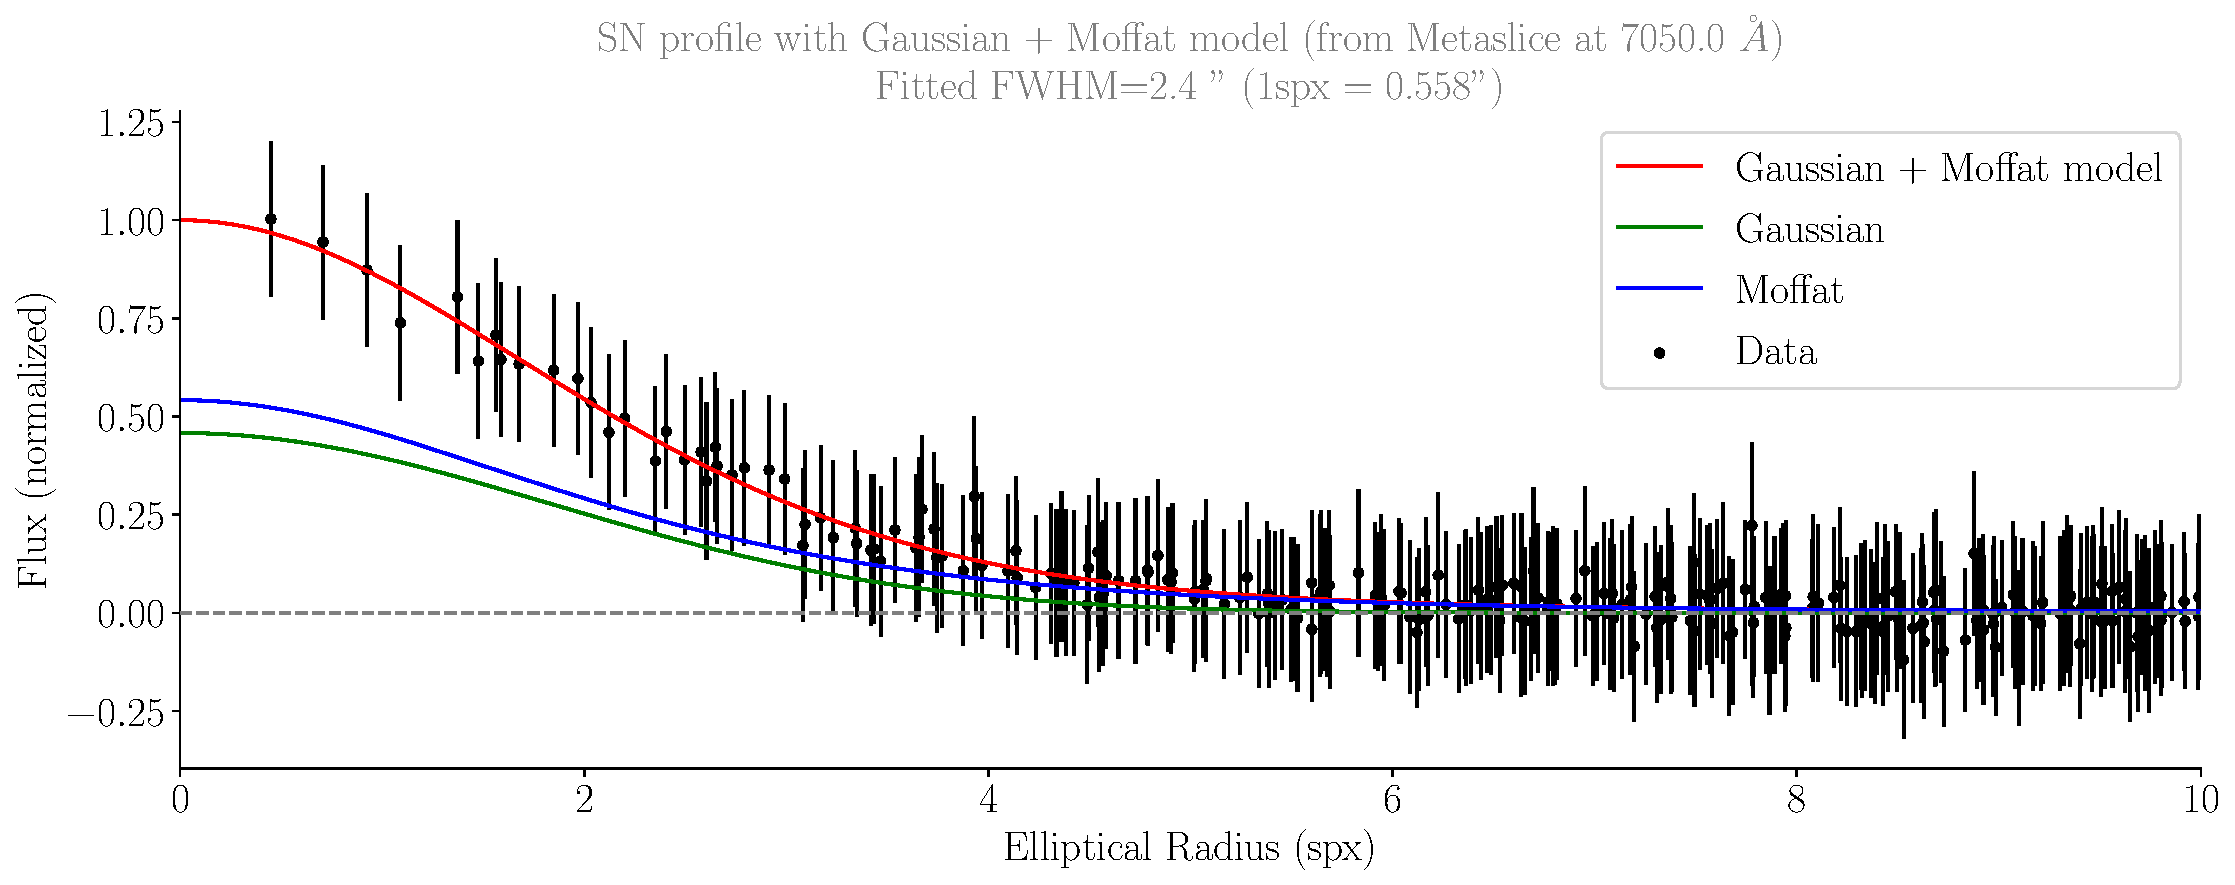
\includegraphics[width=0.99\textwidth]{../figures/07_scene/output_sn_profile_ZTF18accrorf.pdf}
  \caption[Profile radial et modèle de PSF pour une méta-tranche de
  ZTF18accrorf.]{Profile radial et modèle de PSF pour la méta-tranche à
    $7050$\AA\ de ZTF18accrorf. Le flux est ici normalisé à $1$. Les
    points noirs indiquent les données de la méta-tranche du cube
    d'observation de la SEDm, après soustraction du modèle de la galaxie
  et du fond. Les courbes verte, bleue et rouge montrent respectivement
  l'ajustement de la composante gaussienne, Moffat et profil radial
  total du modèle de PSF pour cette méta-tranche. Le trait horizontal en
pointillés indique un fond de ciel à $0$ si cette composante a été
parfaitement soustraite. Les ailes du profil tendant clairement vers
cette valeur, cela nous conforte quant à la qualité d'ajustement de
cette composante. Connaissant la taille d'un spaxel, nous pouvons
également déterminer la largeur à mi-hauteur à cette longueur d'onde, ici
$2\farcs4$.}
  \label{fig:radialprofileZTF18accrorf}
\end{figure}

L'ajustement de l'amplitude de la PSF de la supernova à chaque tranche
nous permet ainsi d'en extraire le spectre, de la même façon qu'avec les
étoiles standards. Nous montrons enfin dans la
Figure~\ref{fig:spectraZTF18accrorf} le spectre extrait de ZTF18accrorf.

\begin{figure}
  \centering
  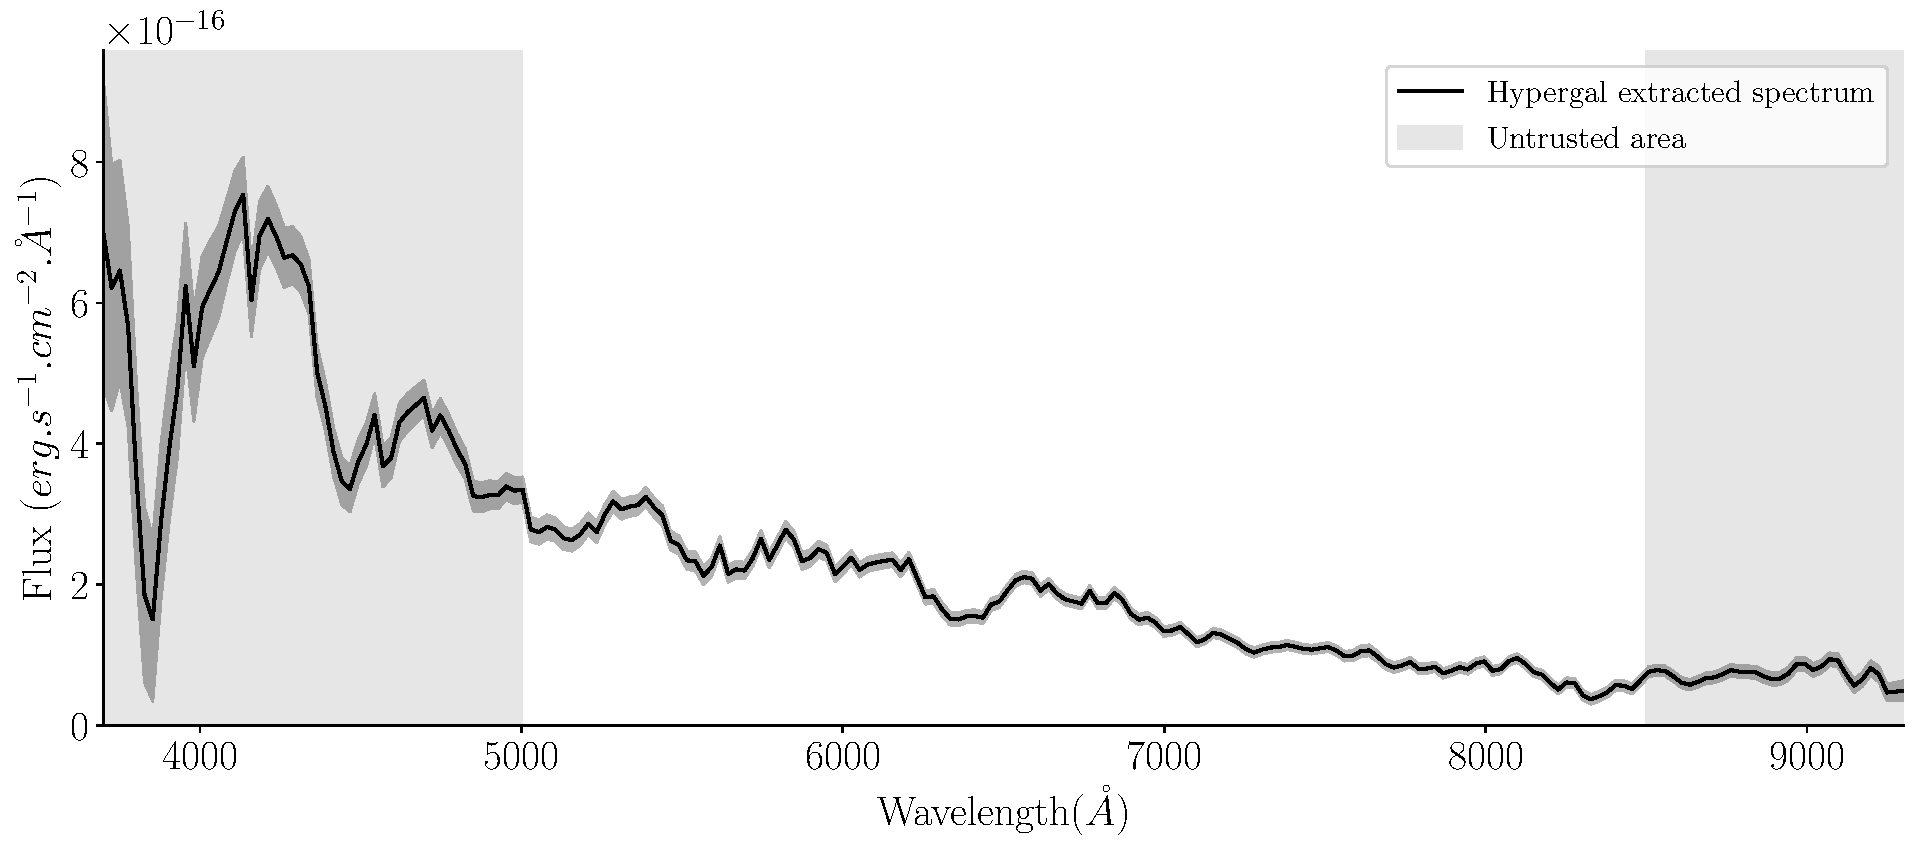
\includegraphics[width=0.99\textwidth]{../figures/07_scene/output_sn_spectra_ZTF18accrorf.pdf}
  \caption[Spectre extrait de ZTF18accrorf avec \hypergal.]{Spectre
    extrait de ZTF18accrorf avec \hypergal. Tout le domaine spectral de
    la SEDm est affiché, et les bandes grises indiquent les zones
    auxquelles nous accordons généralement une faible fiabilité.}
  \label{fig:spectraZTF18accrorf}
\end{figure}

Dans la Figure~\ref{fig:allsourcesZTF18accrorf} nous montrons la
superposition du spectre des 3 composantes (fond, galaxie, supernova),
ainsi que l'ajustement du coefficient de correction $G$ du cube
intrinsèque. L'objectif principal de cette visualisation et de vérifier
une potentielle contamination entre les spectres, par exemple des raies
d'emission de la galaxie, ce qui ne semble pas être le cas ici.
Nous pouvons par ailleurs voir l'évolution chromatique du coefficient $G$,
qui semble corriger dans le cube intrinsèque un excédant d'intensité de la raie d'émission O[III] vers
$5200$\AA, et un déficit d'intensité de la raie H$\alpha$. Bien que nous
n'ayons pas poussé l'analyse de cet effet, nous avons choisi pour le
moment de laisser ce coefficient $G$ libre lors de l'ajustement
linéaire des amplitudes par tranche spectrale, afin d'avoir cette
liberté de correction.
Le modèle de ciel présent dans cette figure correspond au coefficient
de degré $0$ du modèle de fond $b_{0}$ (equation~\ref{eq:backgroundcurved2}).

\begin{figure}
  \centering
  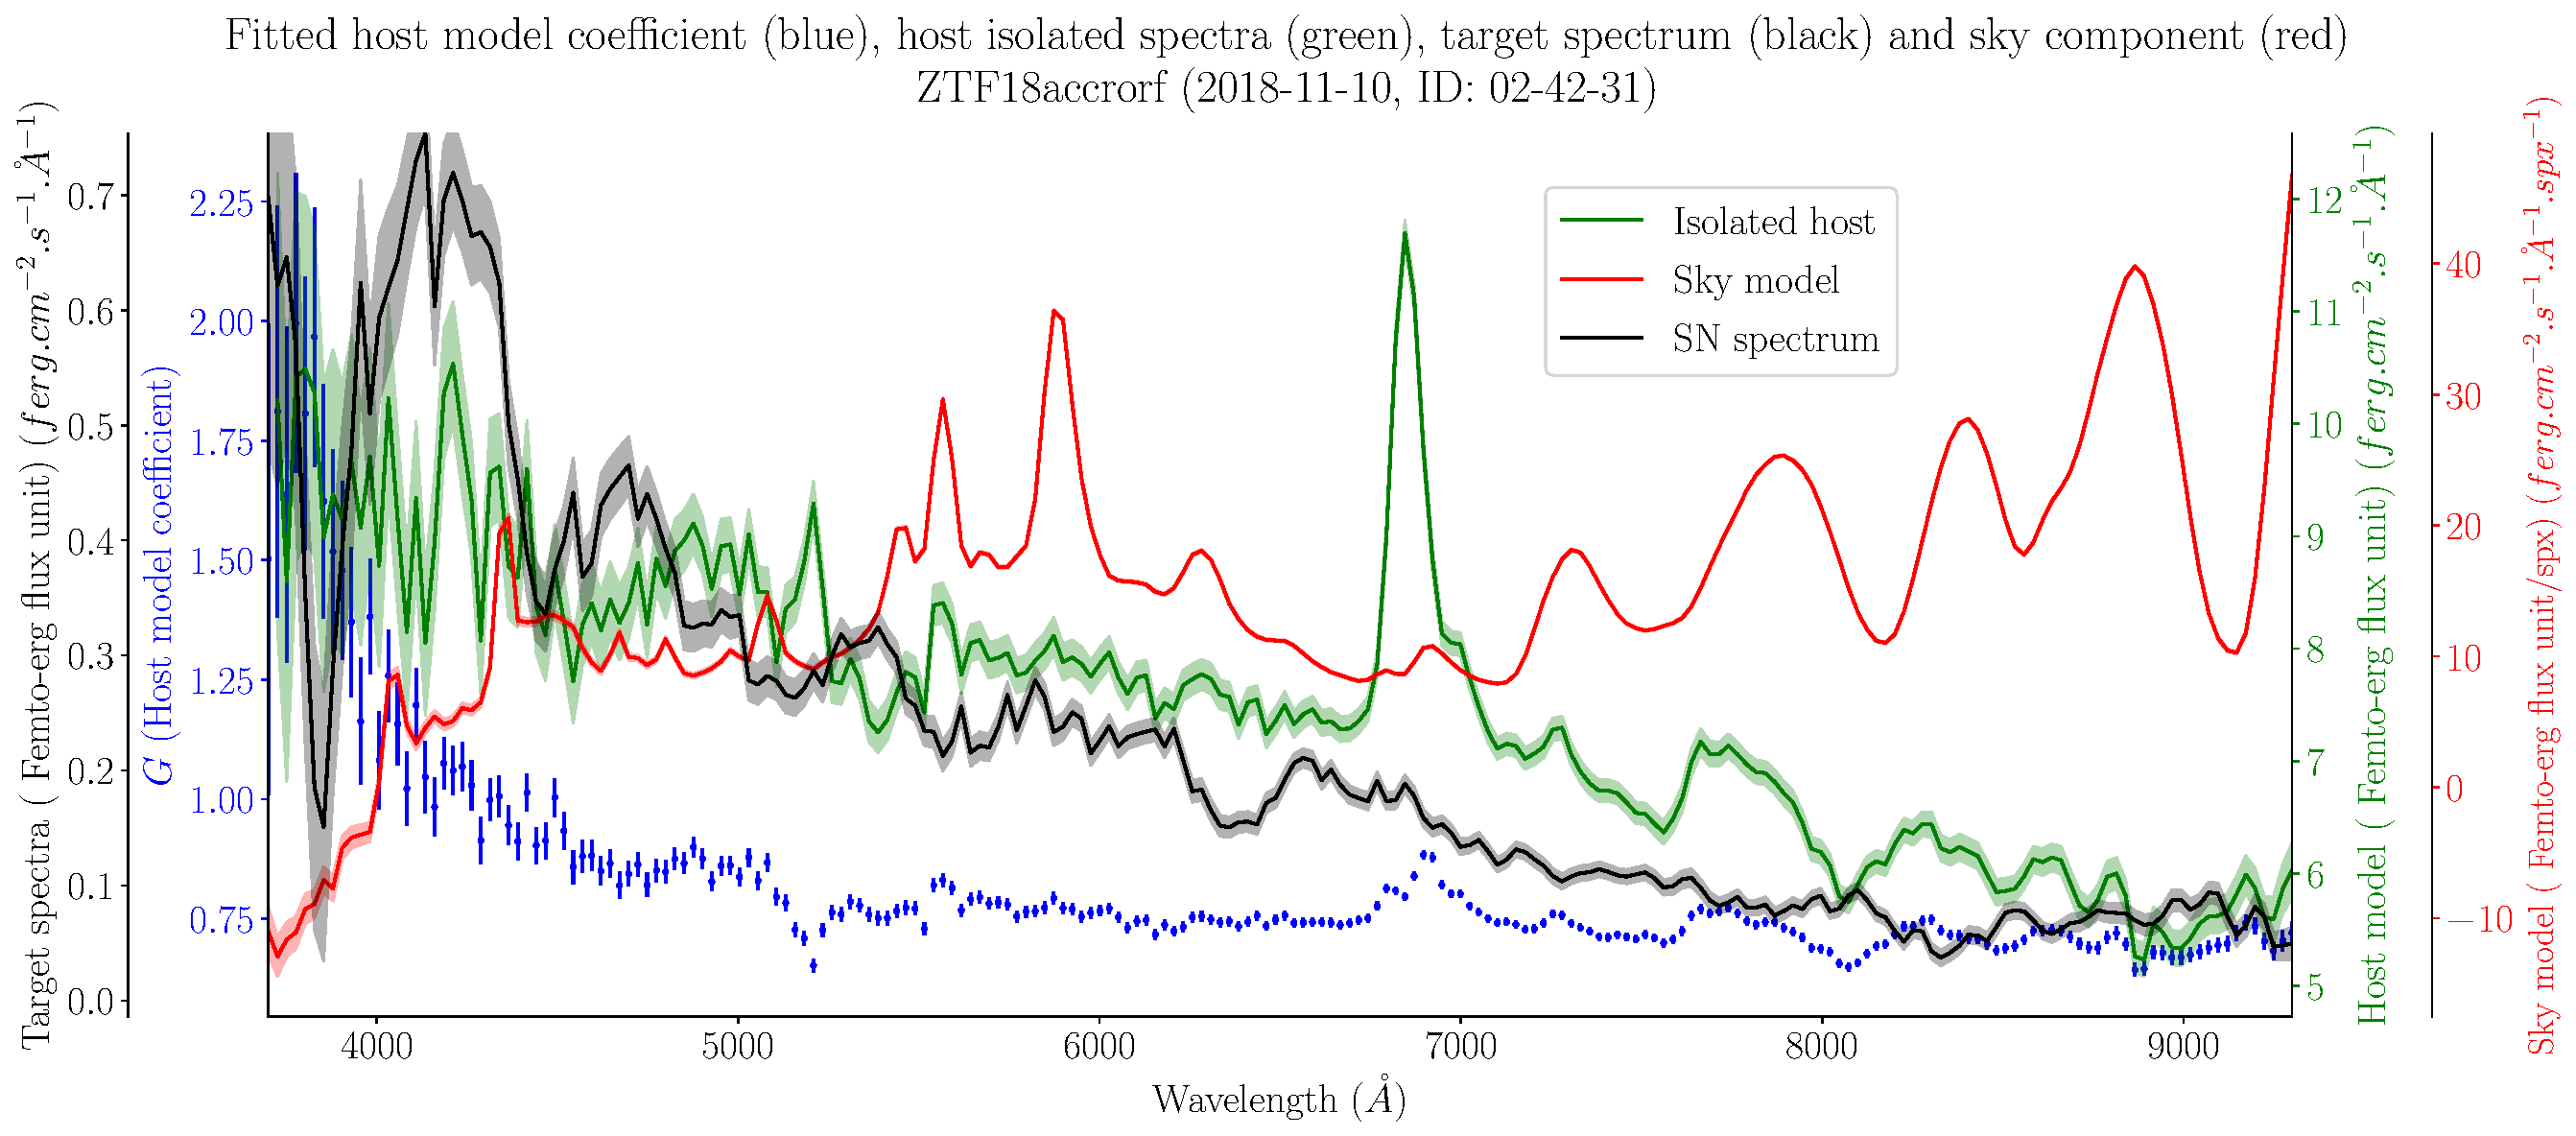
\includegraphics[width=0.99\textwidth]{../figures/07_scene/overlapped_component_ZTF18accrorf.pdf}
  \caption[Superposition du spectre des 3 composantes de la scène
  ZTF18accrorf.]{Superposition du spectre des 3 composantes de la scène d'observation de ZTF18accrorf: fond de
    ciel en rouge,
    galaxie en vert, supernova en noir.
    Nous montrons également l'évolution chromatique de l'ajustement du coefficient de correction $G$ du cube
    intrinsèque. Le but de cette superposition est de mettre en évidence
    l'absence de contamination évidente entre les spectres notamment par
    les raies d'émission de la galaxie. L'évolution du paramètre $G$
    montre l'adaptation de l'intensité des raies O[III] et H$\alpha$ aux observations.}
  \label{fig:allsourcesZTF18accrorf}
\end{figure}

Nous présentons finalement le schéma complet de toute la procédure de
modélisation de scène avec \hypergal. Un script d'automatisation de tout
ce processus est également disponible dans le code du pipeline, prenant
en entrée le nom d'une cible observée avec ZTF (par exemple
ZTF18accrorf), et/ou le chemin d'accès au cube de données. Les
informations relatives à l'évènement transitoire étudié (redshift, RA/DEC) sont
automatiquement récupérées sur le serveur
Fritz\footnote{\url{https://fritz.science/}} \citep{skyportal2019,
  duev2019real, Kasliwal_2019, Duev2021}, mais peuvent également être
imposées en argument. \hypergal est conçu pour être suffisamment
flexible et adaptable à n'importe quel cube 3D.
Par défaut, le pipeline est optimisé avec la librairie de calculs
parallèles \pkg{DASK}\footnote{\url{https://www.dask.org}}
\citep{Dask}.

\begin{landscape}
\begin{figure}
  \centering
  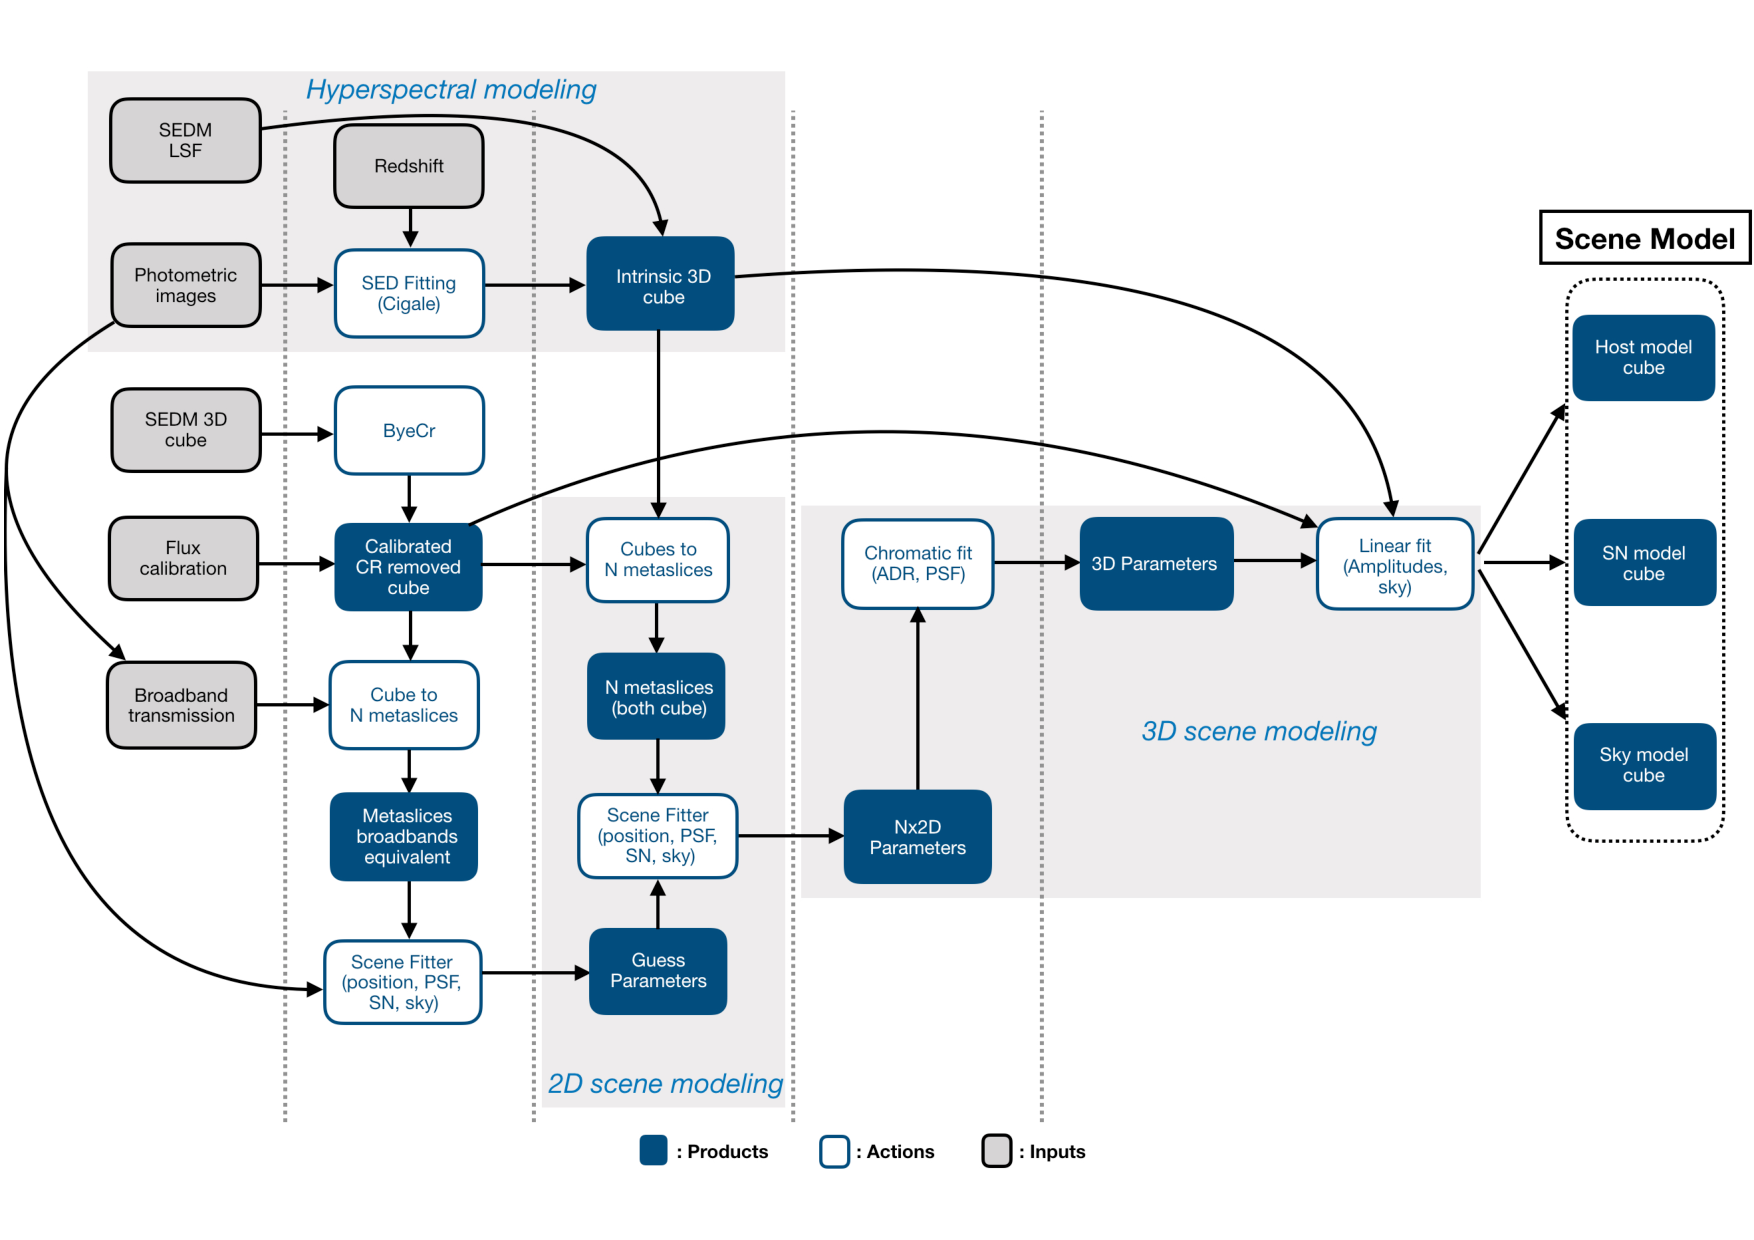
\includegraphics[width=0.99\linewidth]{../figures/07_scene/Fulldaghypergal.pdf}
  \caption{Schéma complet du fonctionnement d'\hypergal. Les étapes sur
    la même verticale sont effectuées simultanément.}
  \label{fig:fulldag}
\end{figure}
\end{landscape}
\section{Classification: \pkg{SNID}}\label{sec:snidclassification}

Bien que le but principal du pipeline \hypergal\ est de
\textit{permettre} la classification du spectre des objets transitoires
observés et non leur classification elle même, nous avons intégré une méthode de classification automatique à l'image de celle
utilisée initialement dans \pkg{pysedm}. Nous utilisons pour cela le
software \pkg{SNID}, présenté dans le chapitre~\ref{sec:snid}. Le
domaine spectral utilisé par défaut pour la classification s'étend entre
$4000$ et $8000$\AA, les modèles utilisés n'étant généralement pas
défini au delà dans l'intervalle de redshift d'observation de ZTF. Bien
que nous ayons présenté notre méfiance quant à la fiabilité des données
en deça de $5000$\AA\ dans les cubes de la SEDm, nous conservons le
spectre extrait jusqu'aux $4000$\AA\ pour la classification en raison des fortes
caractéristiques des SNIae se trouvant dans cet interval spectral
(absorption du silicium, flux plus intense dans le bleu).

Afin de faciliter l'utilisation de \pkg{SNID} initialement écrit en
\pkg{fortran}, nous utilisons une adaptation \pkg{python}:
\pkg{pysnid}\footnote{\url{https://github.com/MickaelRigault/pysnid}}.

Nous montrons dans la Figure~\ref{fig:snidZTF18accrorf} la
classification obtenue du spectre extrait de ZTF18accrorf avec \hypergal, à comparer
avec celle obtenue par extraction sans modélisation de la galaxie hôte
par \pysedm, que nous avons présenté dans la
Figure~\ref{fig:easycaseextractionpysedm}. Initialement, la
classification était plus qu'incertaine, avec un paramètre de qualité
r$lap$ de $4.5$ (le seuil minimal de "bonne qualité" étant 5), et un
redshift estimé de $z=0.178$ (au delà de la profondeur en magnitude de
la SEDm).
La classification avec le spectre extrait par \hypergal\ montre pour le
meilleur modèle un r$lap$ de $12.5$ pour une supernova de type Ia, à un
redshift proche de celui estimé de la galaxie hôte ($z_{snid}=0.040$
contre $z_{host}=0.042$).

Nous présentons également la distribution des $30$ modèles avec un
r$lap>6$, ainsi que le meilleur pour chaque sous-type de supernova
pouvant correspondre au spectre extrait de ZTF18accrorf. Nous pouvons
voir que seuls 2 sous-types semblent compatibles: une Ia-normal, ou une
Ia-91T. Bien que la classification du sous-type soit plus subtile, la
classification de ZTF18accrorf ne présente aucun doute comme étant une
Ia.

\begin{figure}[ht]
  \centering
  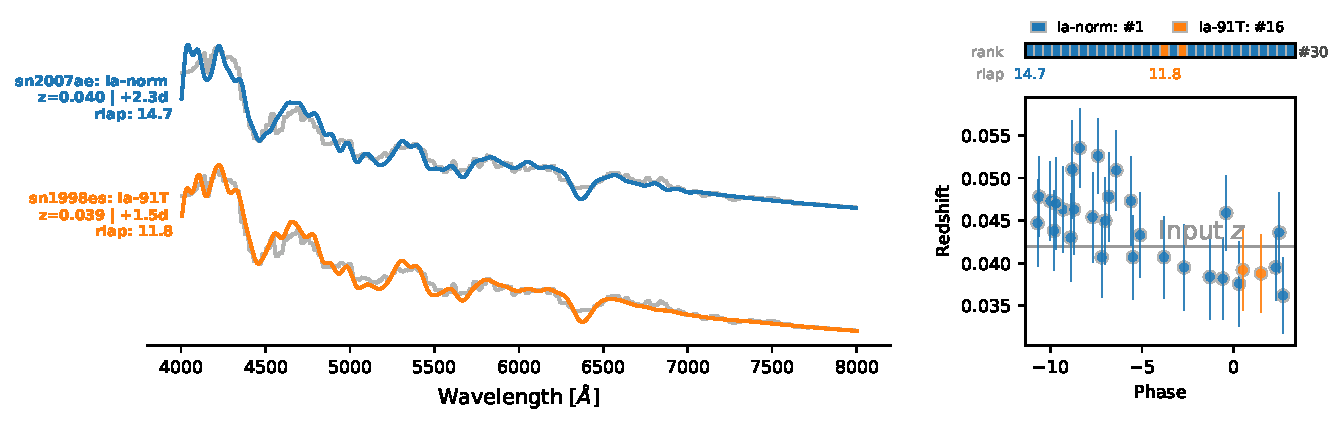
\includegraphics[width=0.95\textwidth]{../figures/07_scene/ZTF18accrorf_snid_typing.pdf}
  \caption[Classification de ZTF18accrorf avec
  \pkg{SNID}]{Classification de ZTF18accrorf avec \pkg{SNID}. \emph{À
      gauche} les modèles ayant le plus haut r$lap$ pour chaque
    sous-type présent dans les $30$ meilleurs modèles. Pour chacun nous
    y montrons le spectre extrait par \hypergal\ en gris, le modèle en couleur, le type et sous-type, le redshift, la phase et
  le r$lap$. \emph{À droite} est présenté la distribution
  redshift/phase des $30$ meilleurs modèles, avec pour le
  sous-type le même code couleur que pour les spectres affichés à gauche.}
  \label{fig:snidZTF18accrorf}
\end{figure}


\section{Cas complexes}
% \label{ssec:xxx}

Bien que le cas utilisé pour présenter le pipeline \hypergal\
(ZTF18accrorf) pouvait donner du
fil à retordre à la méthode d'extraction directe (\pysedm), nous
considérons ce type d'observation comme idéal, avec une séparation assez
net de sa galaxie hôte.

Nous présentons dans cette section quelques cas d'extraction plus
complexes de spectre avec \hypergal, pour des observations où la supernova explose
bien plus proche du bulbe galactique.

Pour toutes les observations que nous présentons ici, l'extraction avec le pipeline
\pysedm\ ne permet de classifier le spectre de la supernova, le coeur de
la galaxie hôte étant extrait en même temps que la source ponctuelle
(voir Figure~\ref{fig:stronghost}).

Nous présenterons successivement pour chaque observation: une visualisation globale de la
modélisation de scène avec le RMS et le pull spectral
à l'instar de la Figure~\ref{fig:fullsceneZTF18accrorf}; l'isolation de
la galaxie hôte dans le cube de données SEDm
et le spectre extrait dans l'ouverture définie dans la section~\ref{ssec:hostextract};
l'isolation de la supernova dans le cube de données SEDm et le spectre
extrait (section~\ref{ssec:snextraction}); la
classification avec \pkg{SNID} (section~\ref{sec:snidclassification}). 

\subsection{ZTF19acbjlnt}

Cette supernova est celle que nous avons présenté à la fin du
chapitre~\ref{ch:sedm}, afin justement d'illustrer le phénomène de
contamination par la galaxie hôte lors d'un alignement avec le bulbe
galactique dans la ligne de visée. La distance apparente entre la
supernova et le centre de la galaxie est d'environ $0\farcs8$, c'est à dire moins de la moitié
de la largeur à mi-hauteur typique de la SEDm, et à un peu plus d'un spaxel
de distance du centre du coeur de la galaxie hôte.
\begin{figure}[ht]
  \centering
  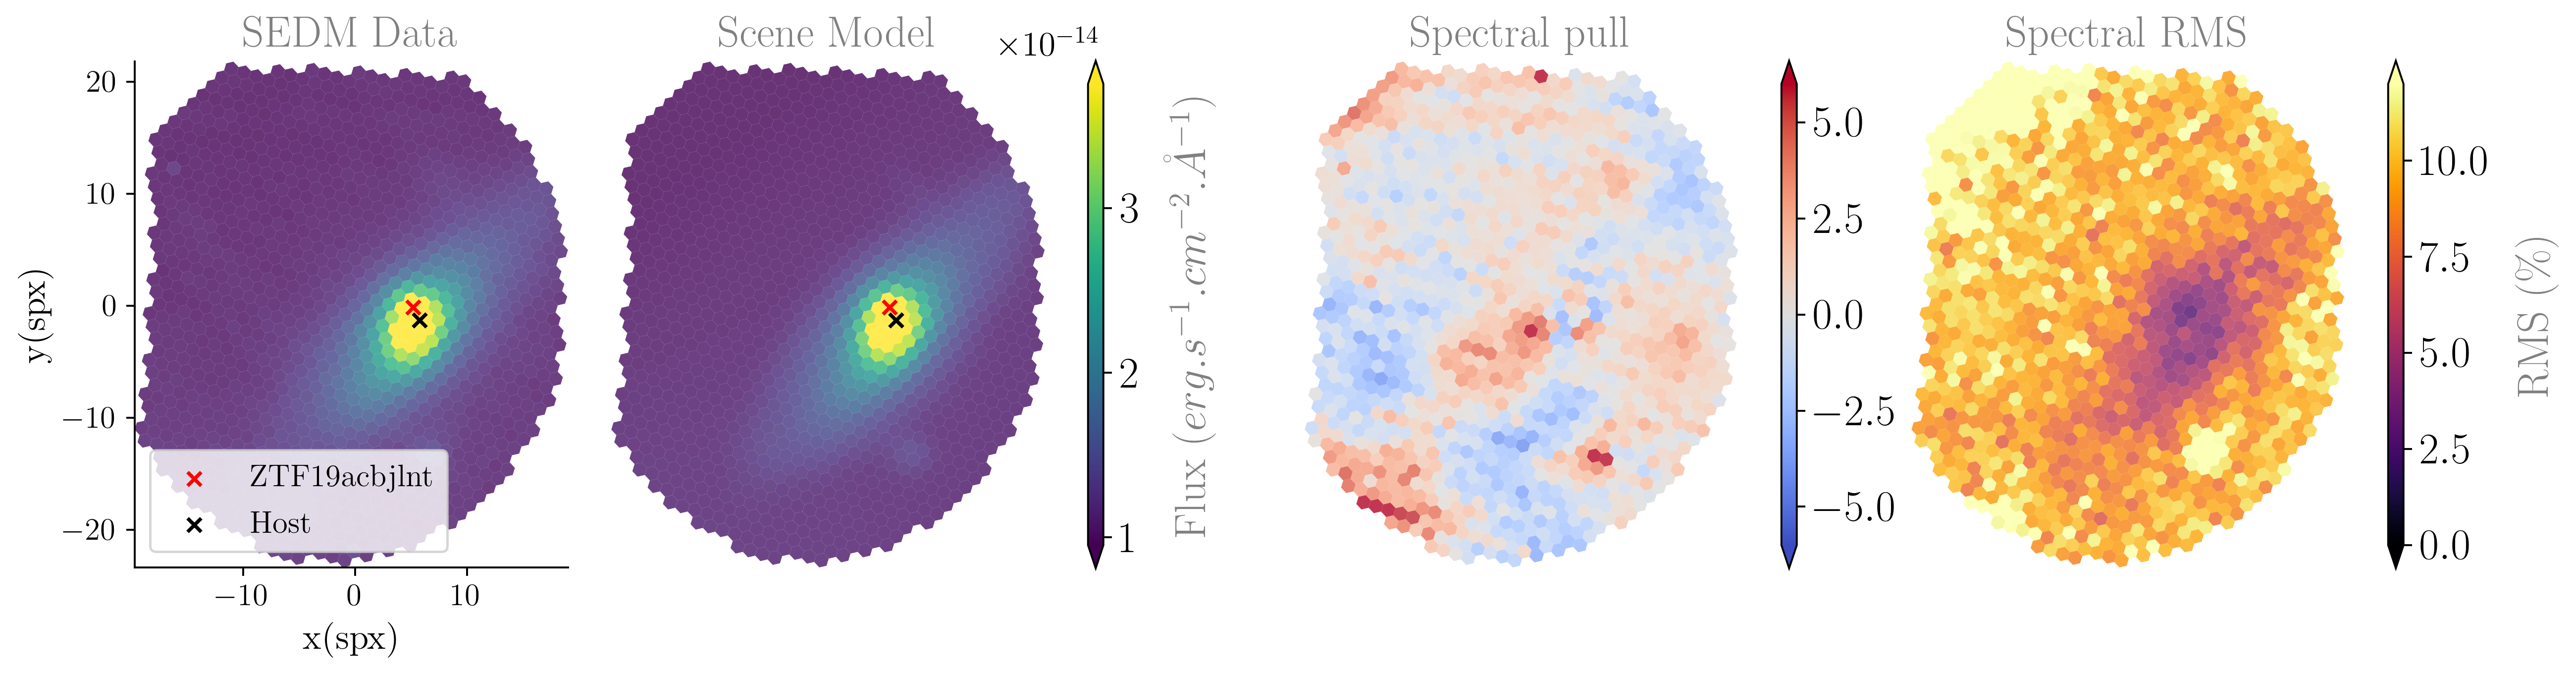
\includegraphics[width=0.9\textwidth]{../figures/07_scene/scene_rmspull_ZTF19acbjlnt.png}
  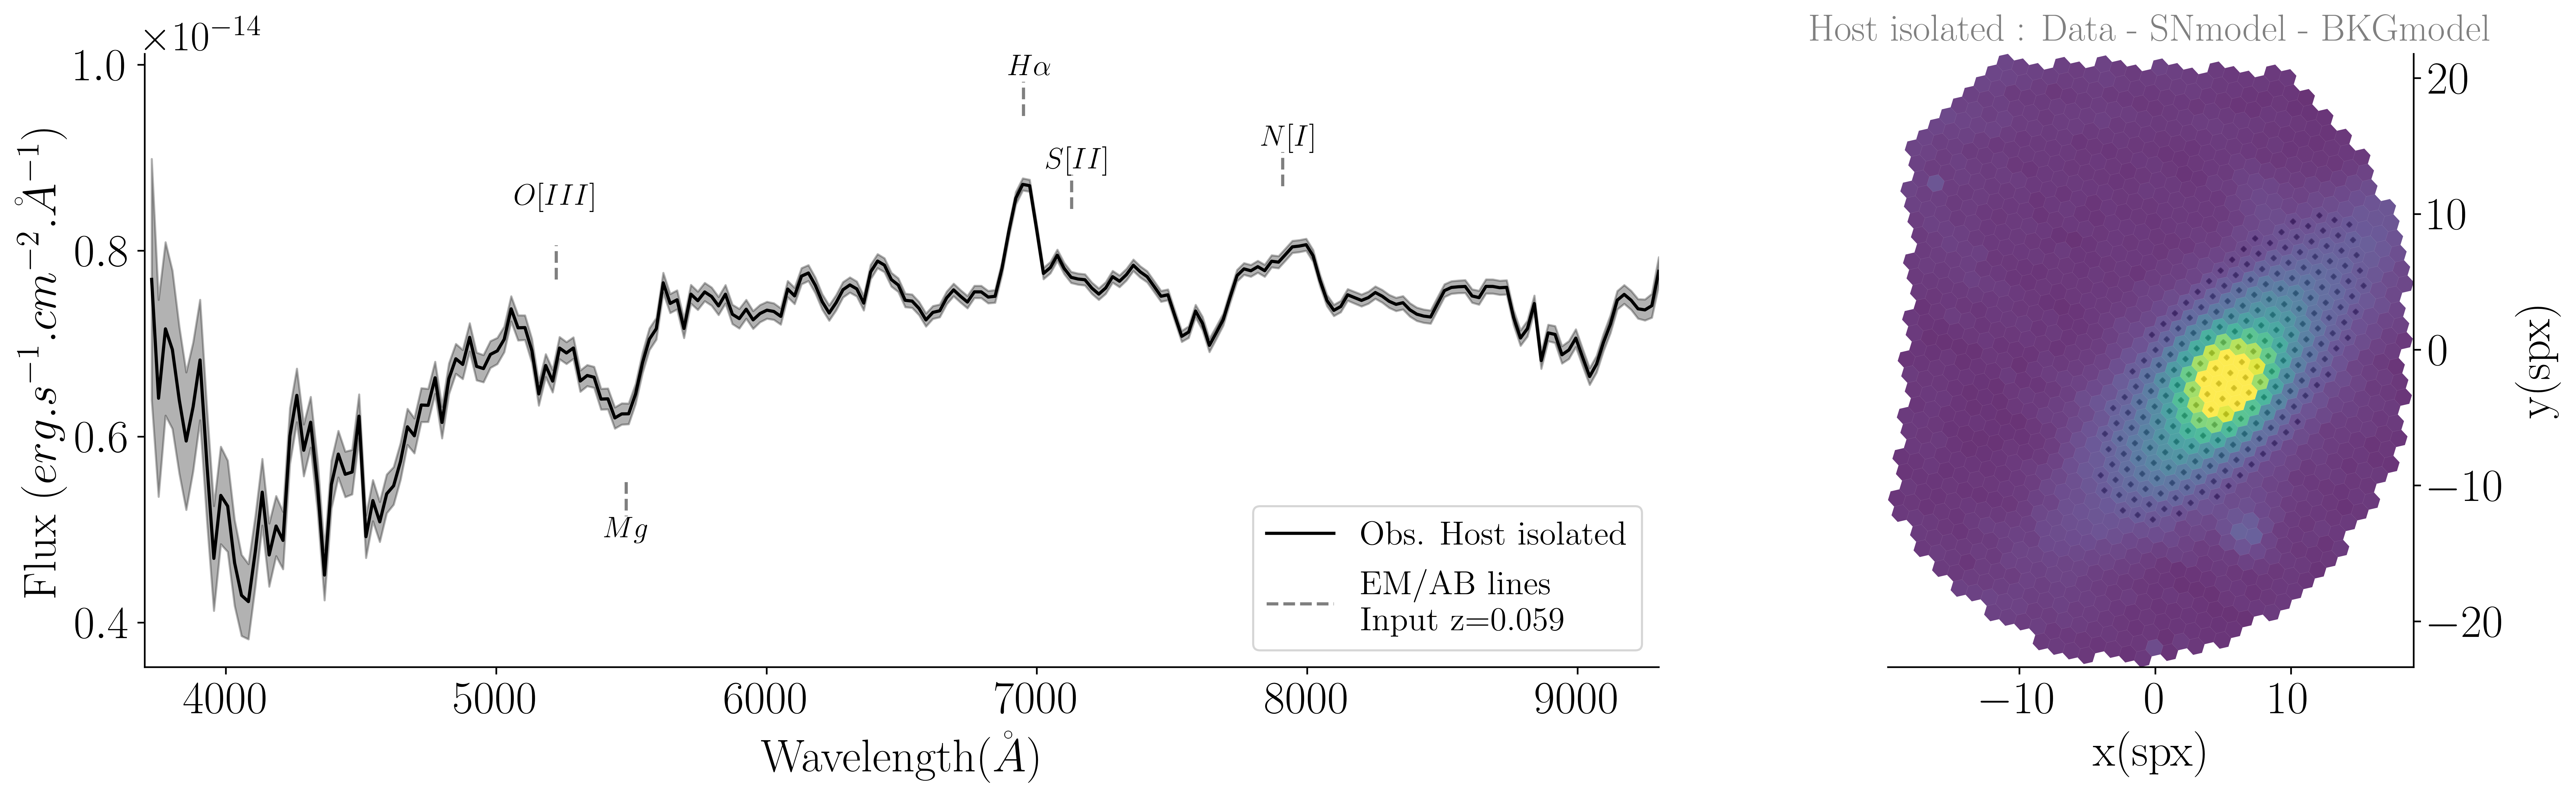
\includegraphics[width=0.85\textwidth]{../figures/07_scene/output_host_ZTF19acbjlnt.png}
  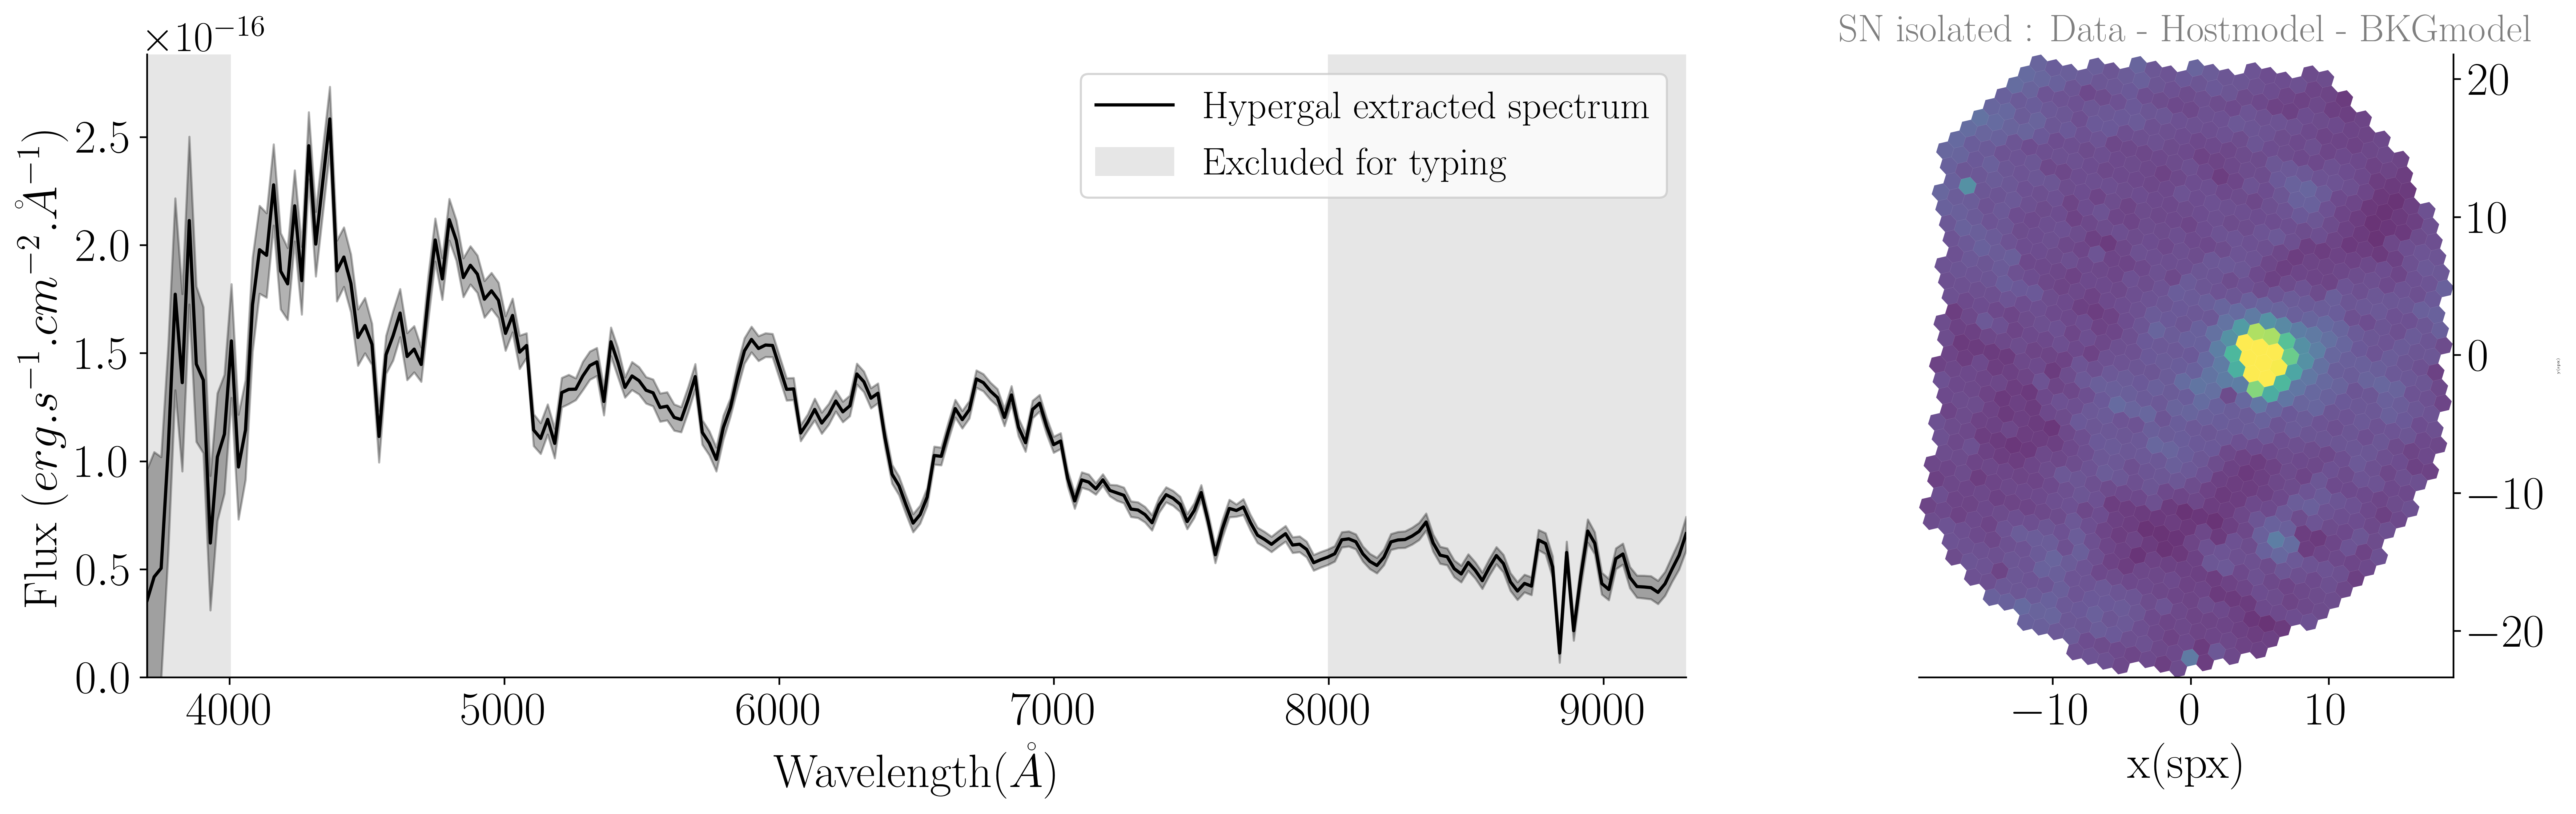
\includegraphics[width=0.85\textwidth]{../figures/07_scene/output_target_ZTF19acbjlnt.png}
  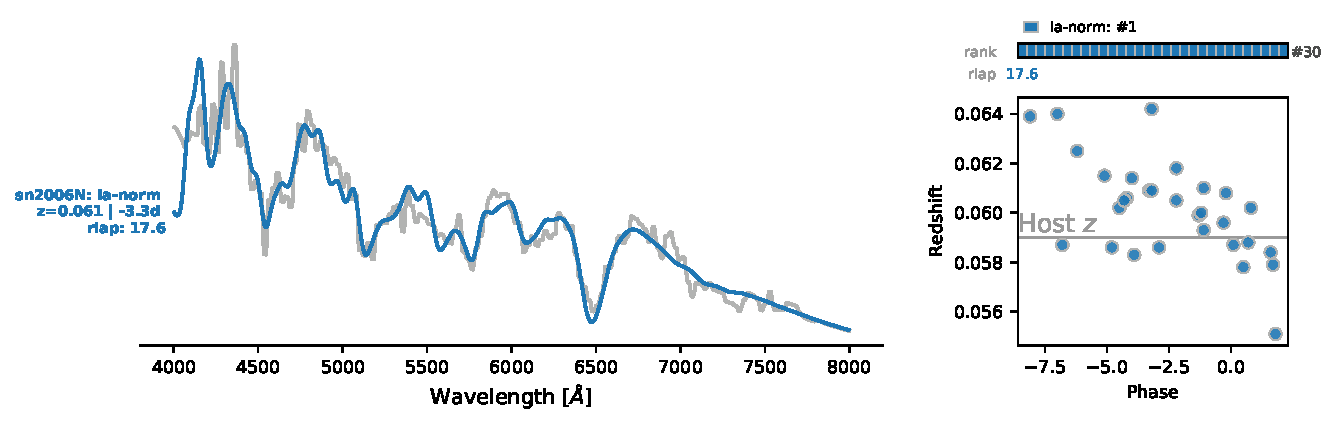
\includegraphics[width=0.85\textwidth]{../figures/07_scene/ZTF19acbjlnt_snid_typing.pdf}
  \caption[Extraction de sources pour ZTF19acbjlnt.]{Extraction de
    sources pour ZTF19acbjlnt avec \hypergal. \emph{De haut en bas}:
    (a) visualisation globale de la modélisation de scène, pull et RMS
    spectraux, (b) l'isolation de la galaxie hôte, (c) l'isolation de
    ZTF19acbjlnt, (d) la classification de ZTF19acbjlnt. La distance apparente entre la
supernova et la galaxie est d'environ $0\farcs8$.}
  \label{}
\end{figure}

\newgeometry{a4paper,left=2.5cm, right=2.5cm, bottom=1.5cm,top=3cm}

\subsection{ZTF19abormno}
\begin{figure}[ht]
  \centering
  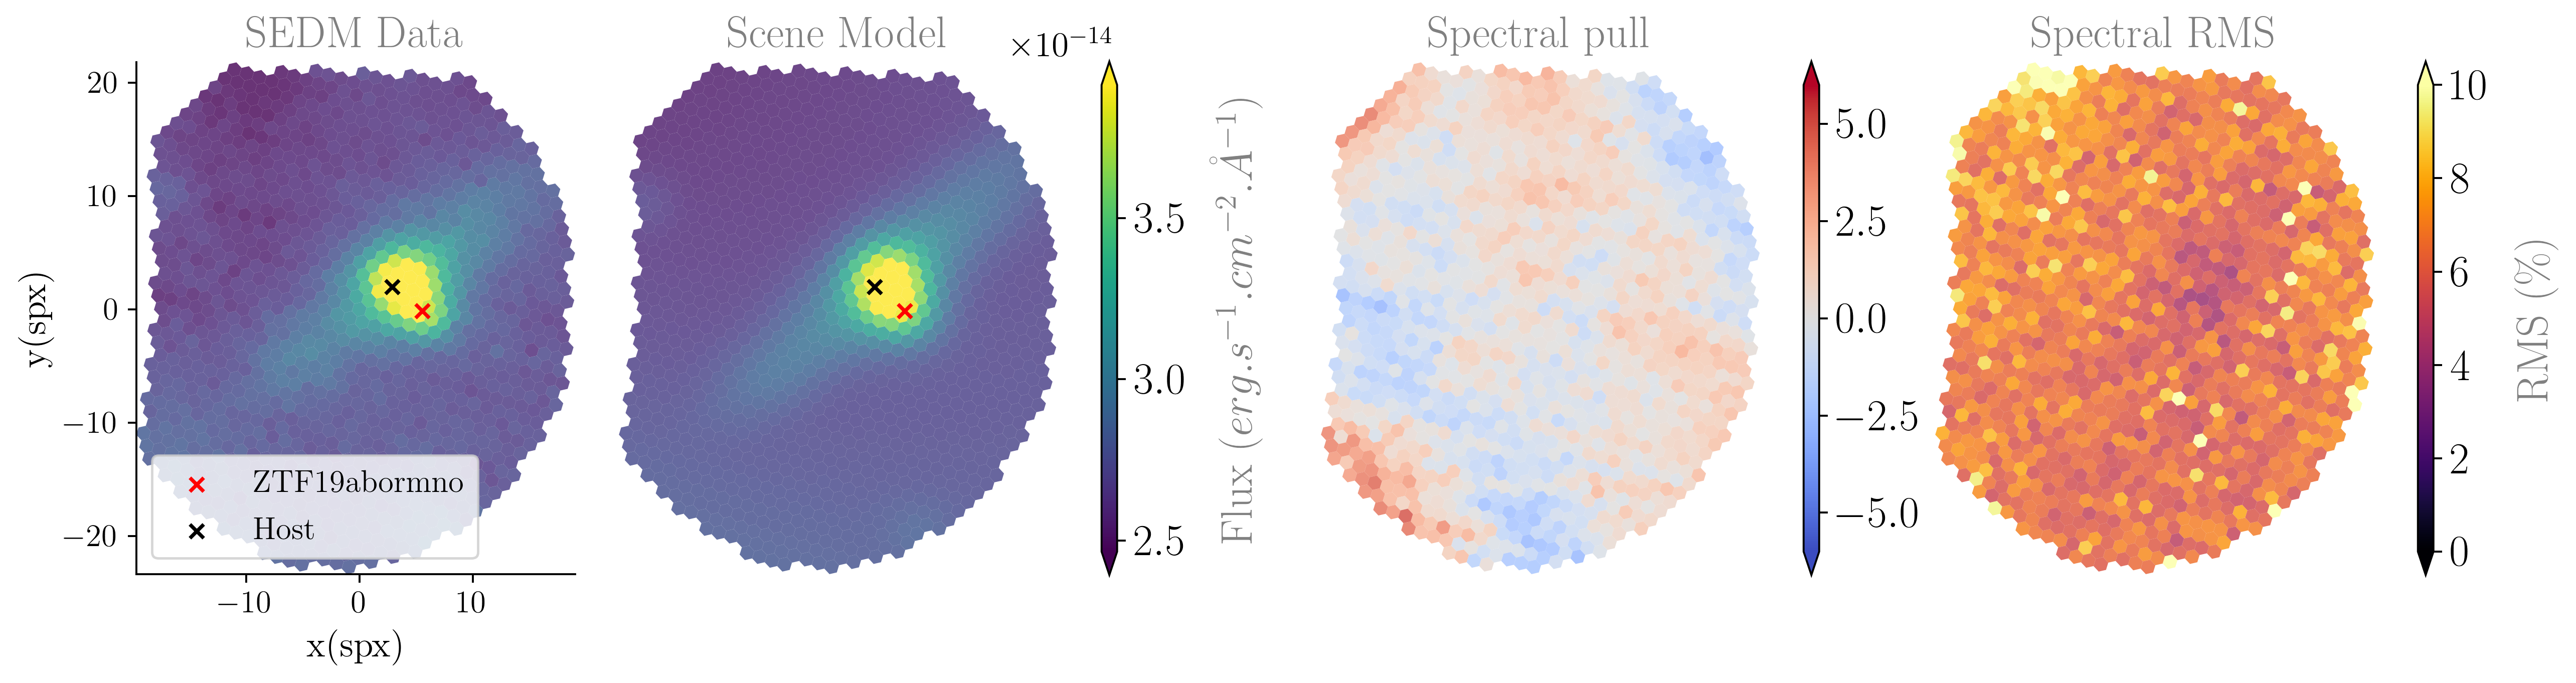
\includegraphics[width=0.9\textwidth]{../figures/07_scene/scene_rmspull_ZTF19abormno.png}
  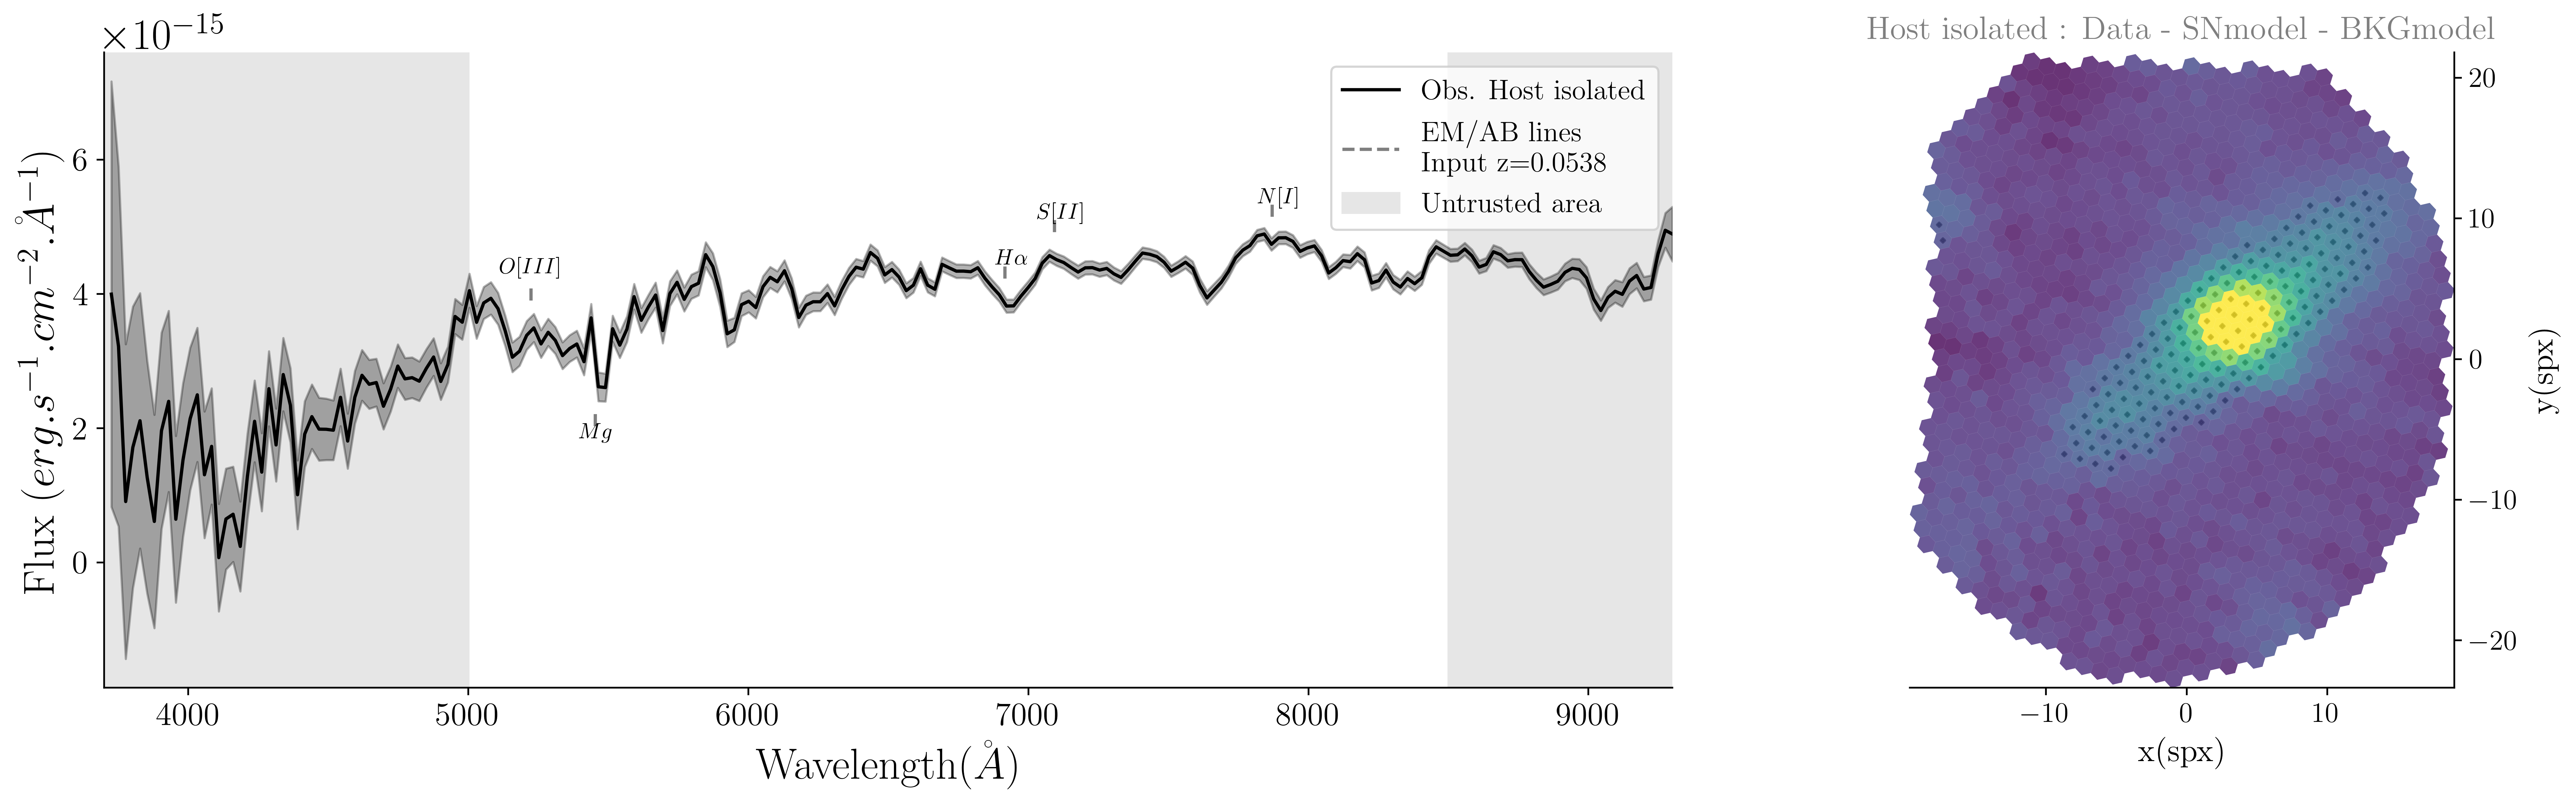
\includegraphics[width=0.85\textwidth]{../figures/07_scene/output_host_ZTF19abormno.png}
  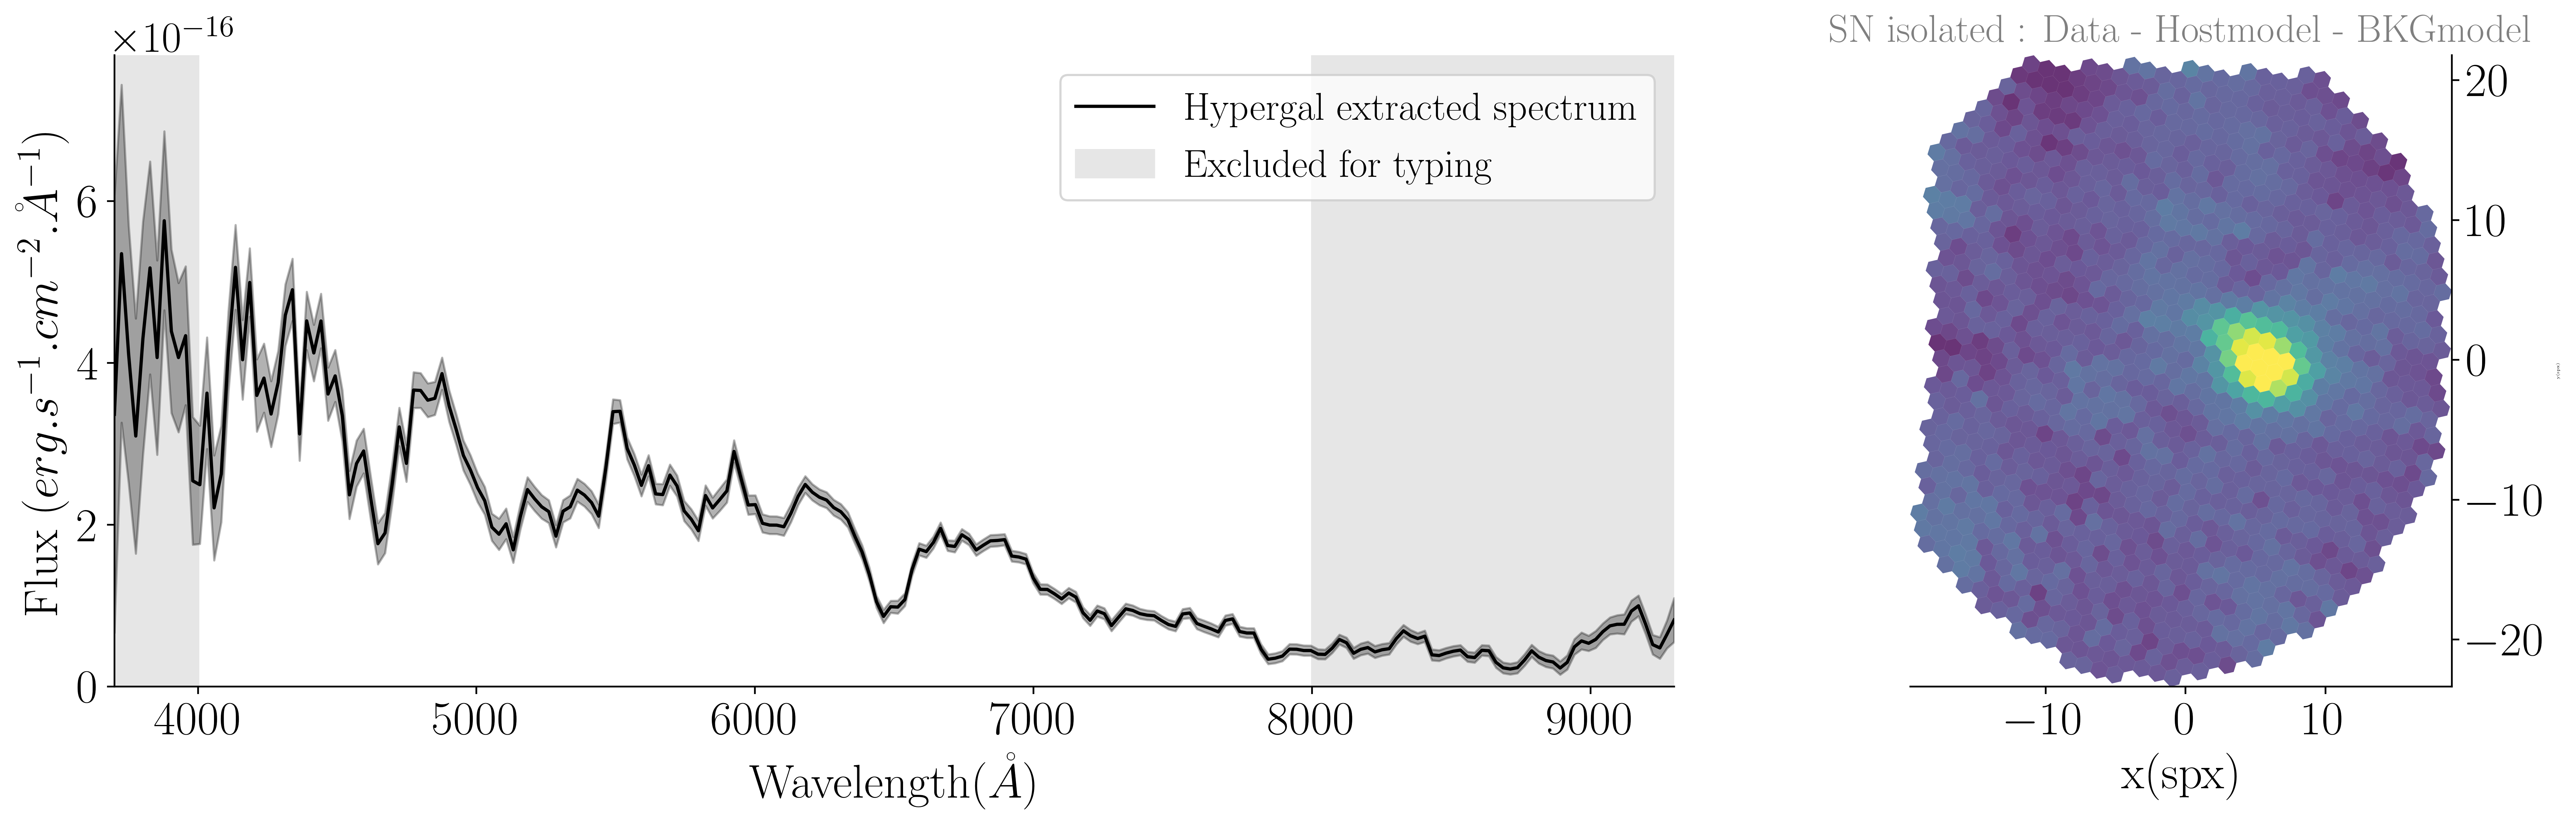
\includegraphics[width=0.85\textwidth]{../figures/07_scene/output_target_ZTF19abormno.png}
  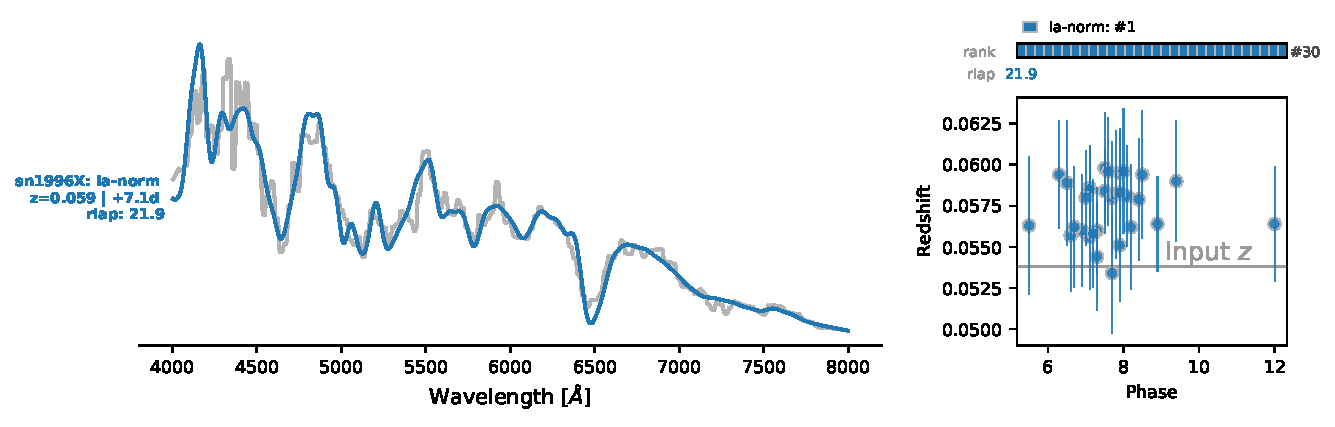
\includegraphics[width=0.85\textwidth]{../figures/07_scene/ZTF19abormno_snid_typing.pdf}
  \caption[Extraction de sources pour ZTF19abormno.]{Extraction de
    sources pour ZTF19abormno avec \hypergal. \emph{De haut en bas}:
    (a) visualisation globale de la modélisation de scène, pull et RMS
    spectraux, (b) l'isolation de la galaxie hôte, (c) l'isolation de
    ZTF19abormno, (d) la classification de ZTF19abormno. La distance apparente entre la
supernova et la galaxie est d'environ $1\farcs5$.}
  \label{}
\end{figure}
\clearpage

\subsection{ZTF20ablhlio}
\begin{figure}[ht]
  \centering
  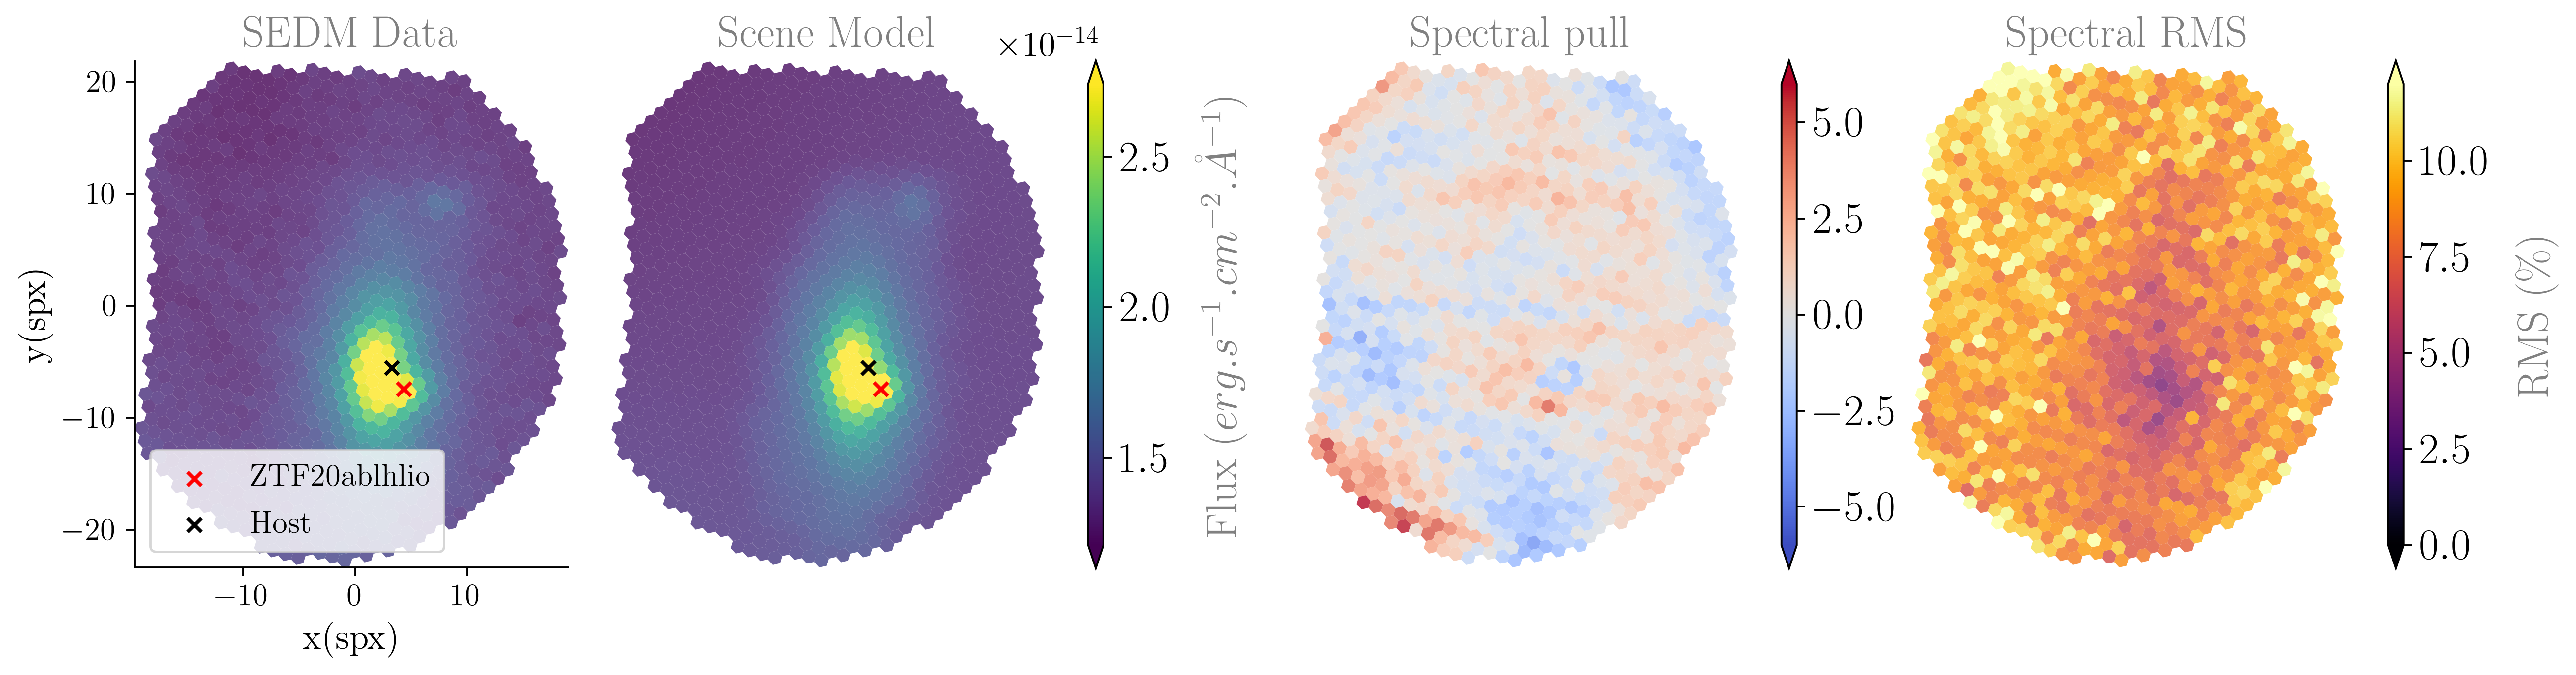
\includegraphics[width=0.9\textwidth]{../figures/07_scene/scene_rmspull_ZTF20ablhlio.png}
  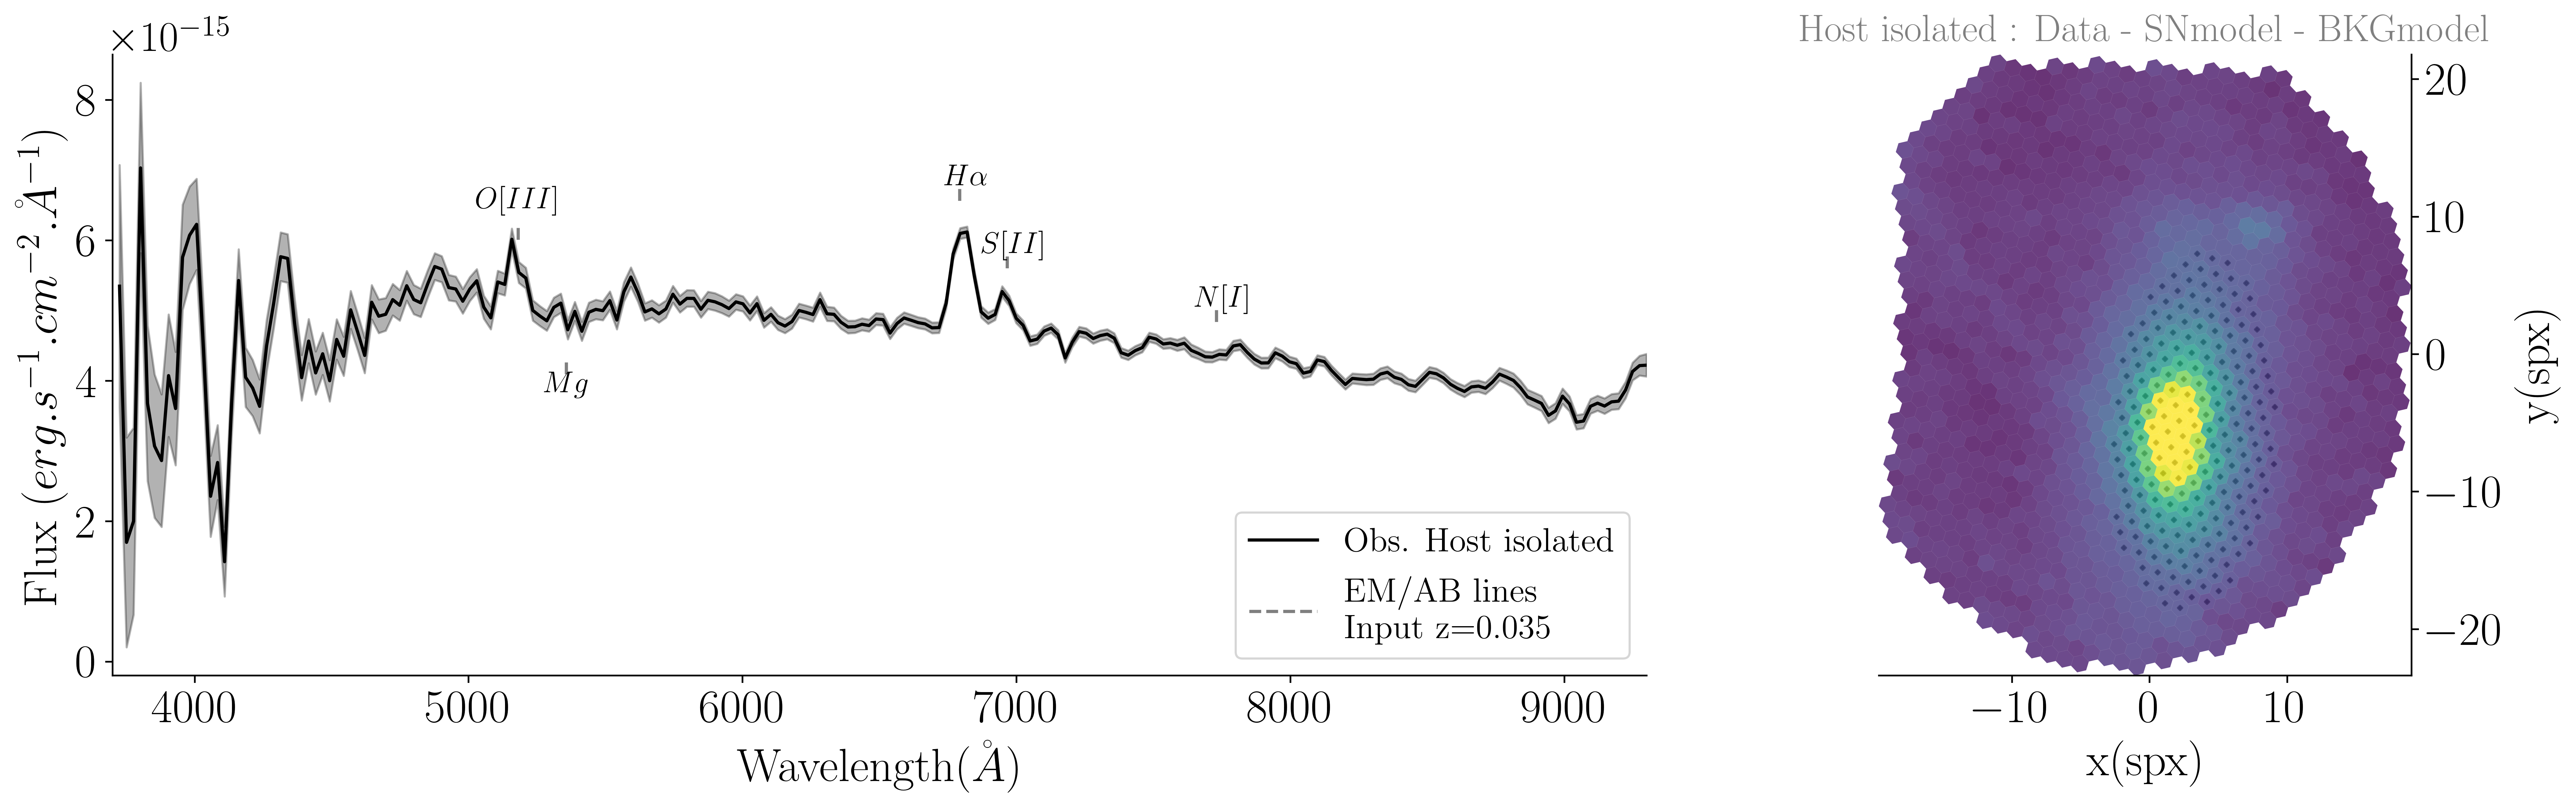
\includegraphics[width=0.85\textwidth]{../figures/07_scene/output_host_ZTF20ablhlio.png}
  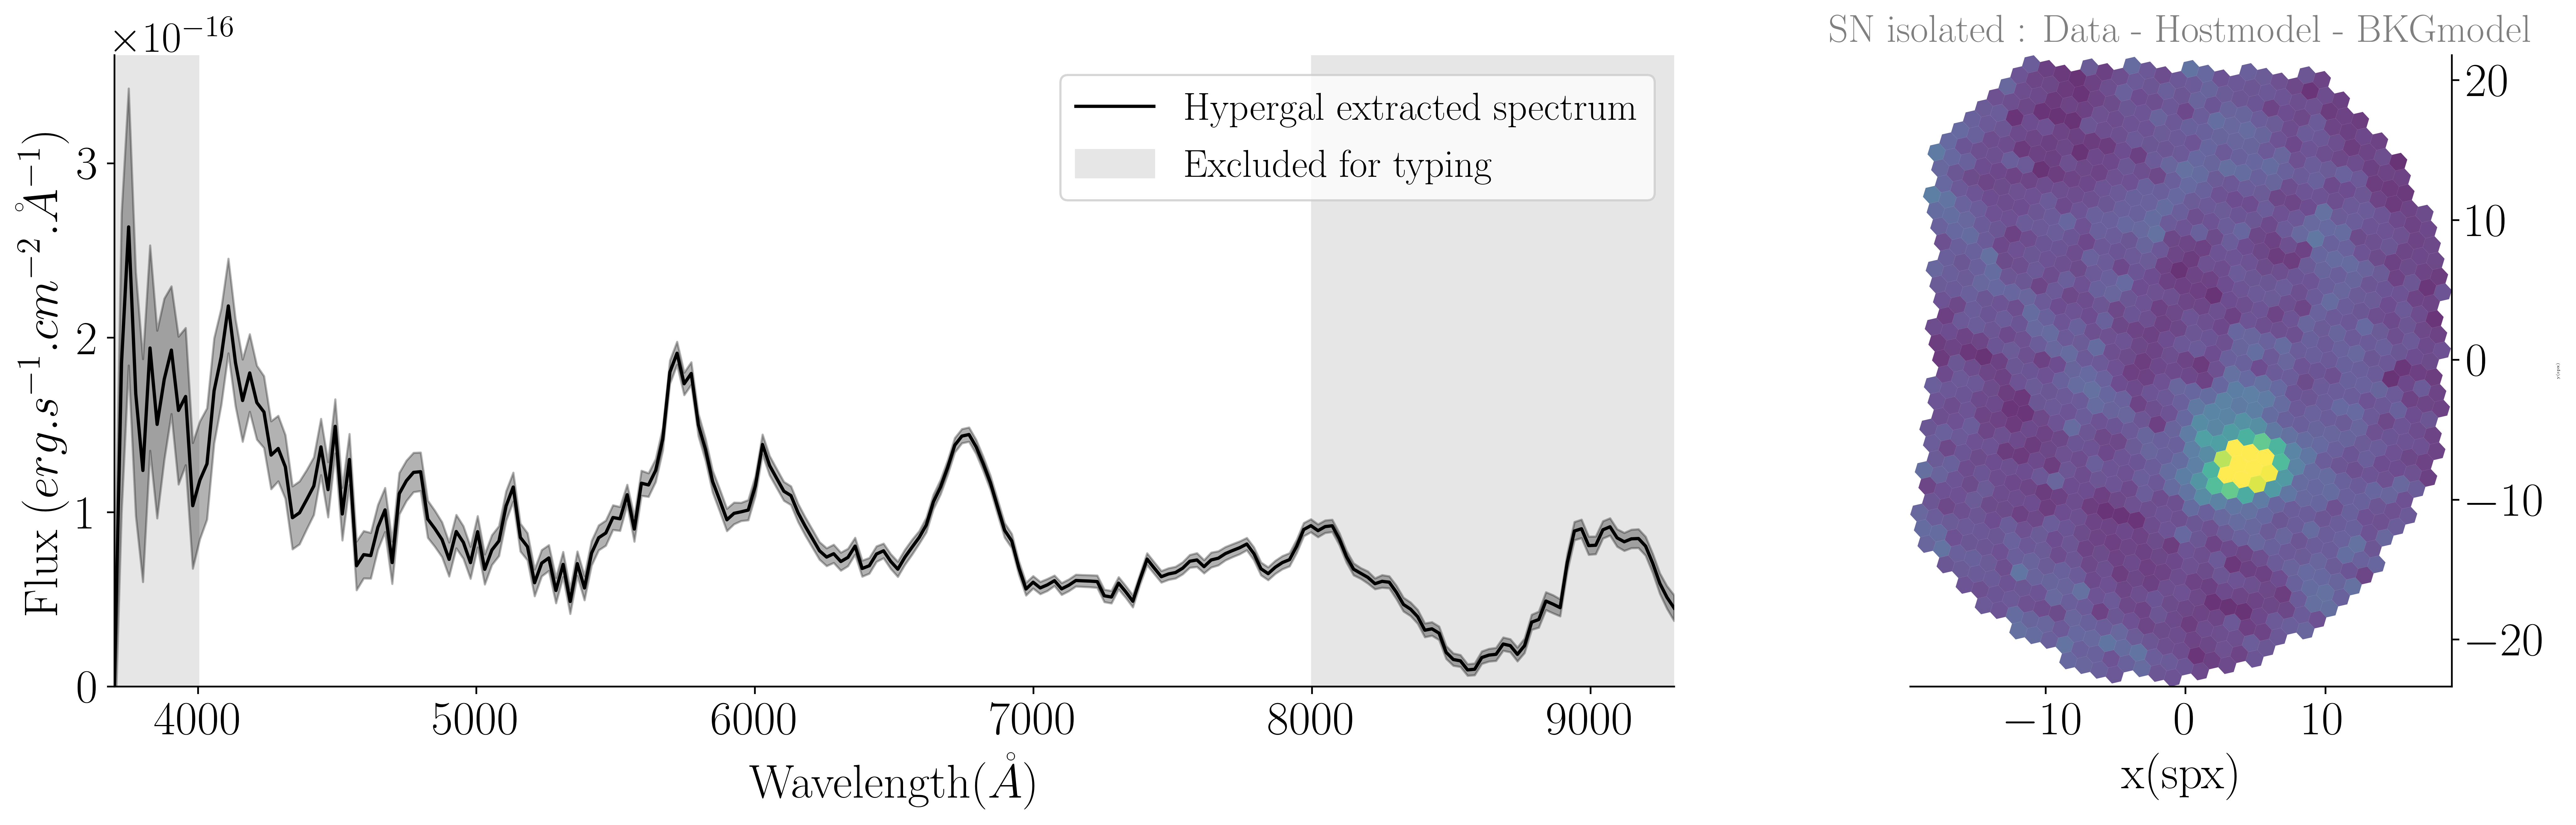
\includegraphics[width=0.85\textwidth]{../figures/07_scene/output_target_ZTF20ablhlio.png}
  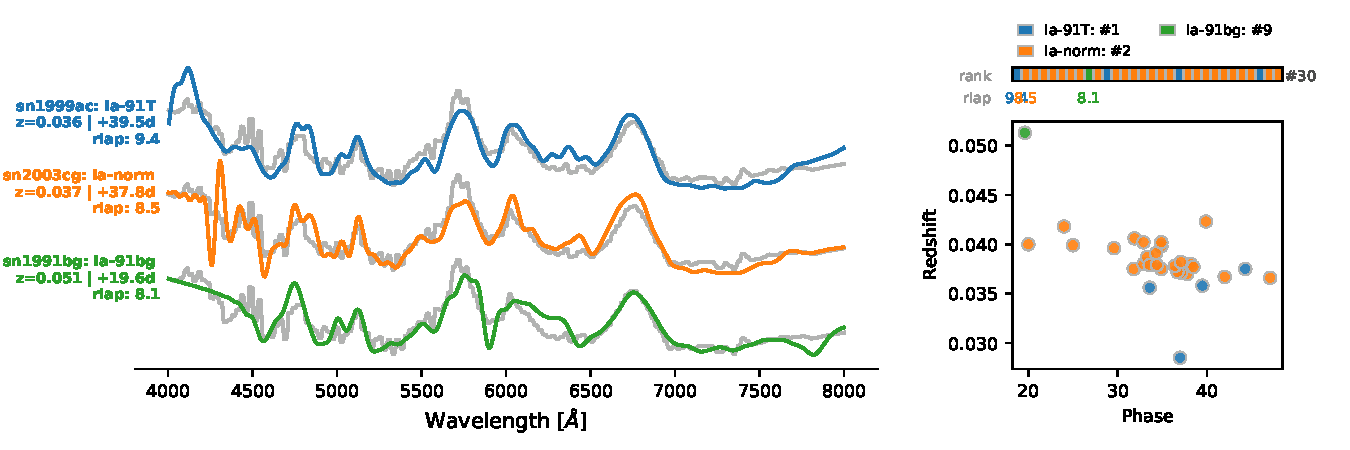
\includegraphics[width=0.85\textwidth]{../figures/07_scene/ZTF20ablhlio_snid_typing.pdf}
  \caption[Extraction de sources pour ZTF19acbjlnt.]{Extraction de
    sources pour ZTF20ablhlio avec \hypergal. \emph{De haut en bas}:
    (a) visualisation globale de la modélisation de scène pull et RMS
    spectraux, (b) l'isolation de la galaxie hôte, (c) l'isolation de
    ZTF20ablhlio, (d) la classification de ZTF20ablhlio. La distance apparente entre la
supernova et la galaxie est d'environ $1\farcs2$.}
  \label{}
\end{figure}

\restoregeometry

%\bibliographystyle{../main/aa_url2}
%\bibliography{99_references}

\end{document}

%%% Local Variables:
%%% mode: latex
%%% TeX-master: t
%%% End:
